\documentclass[12pt,english,a4paper,titlepage,cleardoublepage=empty,dottedtoc]{report}



% % % additions by tompollard START -->

% Overwrite \begin{figure}[htbp] with \begin{figure}[H]
% TODO: delete if images position is awkward
% NOTE: disabled 20170215
%\usepackage{float}
%\let\origfigure=\figure
%let\endorigfigure=\endfigure
%\renewenvironment{figure}[1][]{%
%\origfigure[b]
%}{%
%\endorigfigure
%}

% TP: hack to truncate list of figures/tables.
\usepackage{truncate}
\usepackage{caption}
\usepackage{tocloft}
% TP: end hack

% % % <-- END additions by tompollard



\usepackage{lmodern}
\usepackage{setspace}
\setstretch{1.2}
\usepackage{amssymb,amsmath}
\usepackage{ifxetex,ifluatex}
\usepackage{fixltx2e} % provides \textsubscript
\ifnum 0\ifxetex 1\fi\ifluatex 1\fi=0 % if pdftex
  \usepackage[T1]{fontenc}
  \usepackage[utf8]{inputenc}
\else % if luatex or xelatex
  \ifxetex
    \usepackage{mathspec}
  \else
    \usepackage{fontspec}
  \fi
  \defaultfontfeatures{Ligatures=TeX,Scale=MatchLowercase}
\fi
% use upquote if available, for straight quotes in verbatim environments
\IfFileExists{upquote.sty}{\usepackage{upquote}}{}
% use microtype if available
\IfFileExists{microtype.sty}{%
\usepackage{microtype}
\UseMicrotypeSet[protrusion]{basicmath} % disable protrusion for tt fonts
}{}
\usepackage[unicode=true]{hyperref}
\hypersetup{
            pdftitle={Open Specification of a user-controlled Web Service for Personal Data},
            pdfauthor={G. Jahn},
            pdfkeywords={personal data store; personal data as a service; web service architecture; open specification; masters thesis},
            pdfborder={0 0 0},
            breaklinks=true}
\urlstyle{same}  % don't use monospace font for urls
\ifnum 0\ifxetex 1\fi\ifluatex 1\fi=0 % if pdftex
  \usepackage[shorthands=off,main=english]{babel}
\else
  \usepackage{polyglossia}
  \setmainlanguage[]{english}
\fi

% added 20170205 -->
% NOTE: Replace "english" in "captionsenglish" with the language you use
\addto\captionsenglish{
  \renewcommand{\contentsname}
    {Table of Contents}
}
% added 20170205 <--

\usepackage{color}
\usepackage{fancyvrb}
\newcommand{\VerbBar}{|}
\newcommand{\VERB}{\Verb[commandchars=\\\{\}]}
\DefineVerbatimEnvironment{Highlighting}{Verbatim}{commandchars=\\\{\}}
% Add ',fontsize=\small' for more characters per line
\usepackage{framed}
\definecolor{shadecolor}{RGB}{248,248,248}
\newenvironment{Shaded}{\begin{snugshade}}{\end{snugshade}}
\newcommand{\KeywordTok}[1]{\textcolor[rgb]{0.13,0.29,0.53}{\textbf{#1}}}
\newcommand{\DataTypeTok}[1]{\textcolor[rgb]{0.13,0.29,0.53}{#1}}
\newcommand{\DecValTok}[1]{\textcolor[rgb]{0.00,0.00,0.81}{#1}}
\newcommand{\BaseNTok}[1]{\textcolor[rgb]{0.00,0.00,0.81}{#1}}
\newcommand{\FloatTok}[1]{\textcolor[rgb]{0.00,0.00,0.81}{#1}}
\newcommand{\ConstantTok}[1]{\textcolor[rgb]{0.00,0.00,0.00}{#1}}
\newcommand{\CharTok}[1]{\textcolor[rgb]{0.31,0.60,0.02}{#1}}
\newcommand{\SpecialCharTok}[1]{\textcolor[rgb]{0.00,0.00,0.00}{#1}}
\newcommand{\StringTok}[1]{\textcolor[rgb]{0.31,0.60,0.02}{#1}}
\newcommand{\VerbatimStringTok}[1]{\textcolor[rgb]{0.31,0.60,0.02}{#1}}
\newcommand{\SpecialStringTok}[1]{\textcolor[rgb]{0.31,0.60,0.02}{#1}}
\newcommand{\ImportTok}[1]{#1}
\newcommand{\CommentTok}[1]{\textcolor[rgb]{0.56,0.35,0.01}{\textit{#1}}}
\newcommand{\DocumentationTok}[1]{\textcolor[rgb]{0.56,0.35,0.01}{\textbf{\textit{#1}}}}
\newcommand{\AnnotationTok}[1]{\textcolor[rgb]{0.56,0.35,0.01}{\textbf{\textit{#1}}}}
\newcommand{\CommentVarTok}[1]{\textcolor[rgb]{0.56,0.35,0.01}{\textbf{\textit{#1}}}}
\newcommand{\OtherTok}[1]{\textcolor[rgb]{0.56,0.35,0.01}{#1}}
\newcommand{\FunctionTok}[1]{\textcolor[rgb]{0.00,0.00,0.00}{#1}}
\newcommand{\VariableTok}[1]{\textcolor[rgb]{0.00,0.00,0.00}{#1}}
\newcommand{\ControlFlowTok}[1]{\textcolor[rgb]{0.13,0.29,0.53}{\textbf{#1}}}
\newcommand{\OperatorTok}[1]{\textcolor[rgb]{0.81,0.36,0.00}{\textbf{#1}}}
\newcommand{\BuiltInTok}[1]{#1}
\newcommand{\ExtensionTok}[1]{#1}
\newcommand{\PreprocessorTok}[1]{\textcolor[rgb]{0.56,0.35,0.01}{\textit{#1}}}
\newcommand{\AttributeTok}[1]{\textcolor[rgb]{0.77,0.63,0.00}{#1}}
\newcommand{\RegionMarkerTok}[1]{#1}
\newcommand{\InformationTok}[1]{\textcolor[rgb]{0.56,0.35,0.01}{\textbf{\textit{#1}}}}
\newcommand{\WarningTok}[1]{\textcolor[rgb]{0.56,0.35,0.01}{\textbf{\textit{#1}}}}
\newcommand{\AlertTok}[1]{\textcolor[rgb]{0.94,0.16,0.16}{#1}}
\newcommand{\ErrorTok}[1]{\textcolor[rgb]{0.64,0.00,0.00}{\textbf{#1}}}
\newcommand{\NormalTok}[1]{#1}
\usepackage{longtable,booktabs}
% Fix footnotes in tables (requires footnote package)
\IfFileExists{footnote.sty}{\usepackage{footnote}\makesavenoteenv{long table}}{}
\usepackage{graphicx,grffile}
\makeatletter
\def\maxwidth{\ifdim\Gin@nat@width>\linewidth\linewidth\else\Gin@nat@width\fi}
\def\maxheight{\ifdim\Gin@nat@height>\textheight\textheight\else\Gin@nat@height\fi}
\makeatother
% Scale images if necessary, so that they will not overflow the page
% margins by default, and it is still possible to overwrite the defaults
% using explicit options in \includegraphics[width, height, ...]{}
\setkeys{Gin}{width=\maxwidth,height=\maxheight,keepaspectratio}
% Make links footnotes instead of hotlinks:
\renewcommand{\href}[2]{#2\footnote{\url{#1}}}
\IfFileExists{parskip.sty}{%
\usepackage{parskip}
}{% else
\setlength{\parindent}{0pt}
\setlength{\parskip}{6pt plus 2pt minus 1pt}
}
\setlength{\emergencystretch}{3em}  % prevent overfull lines
\providecommand{\tightlist}{%
  \setlength{\itemsep}{0pt}\setlength{\parskip}{0pt}}
\setcounter{secnumdepth}{3}

% set default figure placement to htbp
\makeatletter
\def\fps@figure{htbp}
\makeatother


% Headers and page numbering
\usepackage{fancyhdr}
% 20170205 changed from \pagestyle{plain}
\pagestyle{fancy}
% added 20170205 -->
\fancyhf{}
\renewcommand{\headrulewidth}{0pt}
\headsep = 60pt
\fancyhead[OL]{\fontsize{10pt}{0pt} \selectfont \textcolor{chaptergrey} \leftmark}
\fancyfoot[C]{\thepage}
% added 20170205 <--

% Table package
\usepackage{ctable}% http://ctan.org/pkg/ctable

% Deal with 'LaTeX Error: Too many unprocessed floats.'
\usepackage{morefloats}
% or use \extrafloats{100}
% add some \clearpage

% % Chapter header
% \usepackage{titlesec, blindtext, color}
% \definecolor{gray75}{gray}{0.75}
% \newcommand{\hsp}{\hspace{20pt}}
% \titleformat{\chapter}[hang]{\Huge\bfseries}{\thechapter\hsp\textcolor{gray75}{|}\hsp}{0pt}{\Huge\bfseries}

% % Fonts and typesetting
% \setmainfont[Scale=1.1]{Helvetica}
% \setsansfont[Scale=1.1]{Verdana}

% FONTS
\usepackage{xunicode}
\usepackage{xltxtra}
\defaultfontfeatures{Mapping=tex-text} % converts LaTeX specials (``quotes'' --- dashes etc.) to unicode
% \setromanfont[Scale=1.01,Ligatures={Common},Numbers={OldStyle}]{Palatino}
% \setromanfont[Scale=1.01,Ligatures={Common},Numbers={OldStyle}]{Adobe Caslon Pro}
%Following line controls size of code chunks
% \setmonofont[Scale=0.9]{Monaco}
%Following line controls size of figure legends
% \setsansfont[Scale=1.2]{Optima Regular}

%Attempt to set math size
%First size must match the text size in the document or command will not work
%\DeclareMathSizes{display size}{text size}{script size}{scriptscript size}.
\DeclareMathSizes{12}{13}{7}{7}

% ---- CUSTOM AMPERSAND
% \newcommand{\amper}{{\fontspec[Scale=.95]{Adobe Caslon Pro}\selectfont\itshape\&}}

% HEADINGS
\usepackage{sectsty}
\usepackage[normalem]{ulem}
\sectionfont{\rmfamily\mdseries\Large\raggedright}
% \subsectionfont{\rmfamily\mdseries\scshape\large}
% \sectionfont{\rmfamily\mdseries\Large}
% \subsectionfont{\rmfamily\mdseries\scshape\normalsize}
\subsubsectionfont{\rmfamily\bfseries\upshape\normalsize}

% added 20170222 -->
% adjust spacng before and after level 4 headline
\usepackage{titlesec}
\titlespacing*{\subsubsection}{0pt}{12pt plus 4pt minus 0pt}{0pt plus 0pt minus 0pt}
% added 20170222 <--

% Set figure legends and captions to be smaller sized sans serif font
\usepackage[font={footnotesize,sf}]{caption}

\usepackage{siunitx}

% Adjust spacing between lines to 1.5
\usepackage{setspace}
% \onehalfspacing
%\doublespacing
\raggedbottom

% Set margins
\usepackage[top=1.5in,bottom=1.5in,left=1.5in,right=1.4in]{geometry}
% \setlength\parindent{0.4in} % indent at start of paragraphs (set to 0.3?)
\setlength{\parskip}{9pt}

% Add space between pararaphs
% http://texblog.org/2012/11/07/correctly-typesetting-paragraphs-in-latex/
% \usepackage{parskip}
% \setlength{\parskip}{\baselineskip}

% Set colour of links to black so that they don't show up when printed
\usepackage{hyperref}
\hypersetup{colorlinks=false, linkcolor=black}

% added 20170130 -->
% to fix URLs not willing to break in bibs
% src https://tex.stackexchange.com/questions/3033/forcing-linebreaks-in-url
\usepackage{url}
\def\UrlOrds{\do\*\do\-\do\~\do\'\do\"\do\-}%
\makeatletter
\g@addto@macro{\UrlBreaks}{\UrlOrds}
\makeatother
% added 20170130 <--

% Tables
\usepackage{booktabs}
\usepackage{threeparttable}
\usepackage{array}
\newcolumntype{x}[1]{%
>{\centering\arraybackslash}m{#1}}%

% Allow for long captions and float captions on opposite page of figures
% \usepackage[rightFloats, CaptionBefore]{fltpage}

% Don't let floats cross subsections
% \usepackage[section,subsection]{extraplaceins}


% Chapter styling
% src: https://github.com/chiakaivalya/thesis-markdown-pandoc/blob/master/preamble.tex#L26
\usepackage[grey]{quotchap}
\makeatletter
\renewcommand*{\chapnumfont}{%
  \usefont{T1}{\@defaultcnfont}{b}{n}\fontsize{80}{100}\selectfont% Default: 100/130
  \color{chaptergrey}%
}
\makeatother


% added 20170205 -->
% make block quote latin again
\let\origquote\quote
\let\endorigquote\endquote
\renewenvironment{quote}{%
    \origquote
    \itshape
}
{\endorigquote}
% added 20170205 <--


% added 20170217 -->
% to reduce font size in code
\DefineVerbatimEnvironment{Highlighting}{Verbatim}{fontsize=\small,commandchars=\\\{\}}
% added 20170217 <--

\title{Open Specification of a user-controlled Web Service for Personal Data}
\providecommand{\subtitle}[1]{}
\subtitle{Master Thesis}
\author{G. Jahn}
\date{\today}

\begin{document}
\maketitle
\begin{abstract}
Often data is referred to as \emph{the oil of the 21st century}. But
recovering petroleum or coal is governed by certain rules and
legislation, while vast amounts of personal data are harvested from all
sorts of resources with no working restrictions or asking for
permission. Well air-conditioned data centers are mining around the
clock via dozens of CPUs. Eager to discover even the tiniest
correlations worth interpreting in enormous haystacks that are filled
with data belonging to millions of individuals, who have no knowledge of
those computations. But these very computations, and thus their
developers, almost inevitably and without restraints discriminate
against these so called \emph{data subjects}. Such practices cannot be
accepted because these haystacks contain actual identities of human
beings including their personalities but still getting recklessly
monetized. To address this issue and reduce the possibility of
discrimination, third parties have to be supplied with the least amount
of data in order to stay functional. That is, data owners must be in
charge of deciding which entity has access to what personal data of
theirs. This project aims to specify a personal data service that
empowers its user to regain full control over her personal data. It
facilitates the regulation of data flows and provides detailed
information on where the data goes so that a \emph{data subject} can
become her own data broker. In order to trust such a service, the user
must be able to look inside and see for herself if it behaves in
unexpected ways. Therefore the specification and all implementations are
being open sourced and developed transparently in public, which also
encourages self-hosting.
\end{abstract}

% added 20170204 -->
% moved from cover to separate page
\pagenumbering{Roman}
\addcontentsline{toc}{chapter}{Acknowledgement}
\section*{Acknowledgement}
I'm thanking my Haekelschmein and my internet provider. TODO My
other/better half (significant other) for having my back through the
whole time My parents for letting/allowing me to get this fare.
\newpage
% moved from cover 20170204 <--


{
\setcounter{tocdepth}{1}
% added 20170205 -->
% suppress fancyheader
\pagestyle{plain}
% added 20170205 <--
\tableofcontents
}
% added 20170129 -->
\newpage
\addcontentsline{toc}{chapter}{List of Tables}
% added 20170129 <--
\listoftables
% added 20170129 -->
\newpage
\addcontentsline{toc}{chapter}{List of Figures}
% added 20170129 <--
\listoffigures
% added 20170205 -->
% to fix page numbering
\newpage
% added 20170205 <--
% added 20170205 -->
\pagenumbering{arabic}
% added 20170205 <--
\newpage

\begin{center}
\thispagestyle{empty}
\setcounter{page}{0}
This page intentionally left blank
\end{center}\newpage

\chapter{Introduction}\label{introduction}

\section{Motivation}\label{motivation}

Nowadays, it is difficult to find a business that does not collect data
about something; humans are particular targets of choice for the
\emph{Big Data Movement}
{[}\protect\hyperlink{ref-web_2016_privacy-international-about-big-data}{1}{]}.
Since humans are all individuals, they are distinct from each other.
While subsets of individuals might share a minor set of attributes, the
majority is still very unique to an individual, given that the overall
variety of attributes is complex. That small amount of similarity might
seem to be less important, due to the nature of inflationary occurrence,
but the opposite turns out to be true. These similarities allow to
determine the individuals who are part of a subset and the ones who
aren't. Stereotypical patterns are applied to these subsets and thus to
all related individuals. This enriched information is then used to help
predict outcomes of problems or questions related to these individuals.
In other words, searching for causation where in best the case one might
find correlations. This is also known as \emph{discrimination}, which

\begin{quote}
{[}\ldots{}{]} refers to unfair or unequal treatment of people based on
membership to a category or a minority, without regard to individual
merit
{[}\protect\hyperlink{ref-paper_2008_discrimination-aware-data-mining}{2},
p. 1{]}.
\end{quote}

When interacting - directly as well as indirectly - with each other,
discrimination of human beings is a serious issue in our society, but
also when humans leverage computers and algorithms to uncover formerly
unnoticed information in order to inform their decision making. For
example, when qualifying for a loan, hiring employees, investigating
crimes or renting flats. The decision to approve or deny is based on
computed data about the individuals in question
{[}\protect\hyperlink{ref-book_2015_ethical-it-innovation}{3}, Chap.
5.6{]}, which is merely discrimination on a much larger scale and with
less effort (almost parenthetically). The described phenomenon is
originally referred to as \emph{Bias in computer systems}
{[}\protect\hyperlink{ref-paper_1996_bias-in-computer-systems}{4}{]}.
What at first seems like machines going rouge on humans is, in fact, the
\emph{cognitive bias}
{[}\protect\hyperlink{ref-wikipedia_2016_cognitive-bias}{5}{]} of human
nature, modeled into machine executable language and built to reveal the
patterns their creators were looking for. The \emph{``Inheritance of
humanness''} {[}\protect\hyperlink{ref-web_2016_big-data-is-people}{6},
Sec. 2{]}, so to say.

In addition to the identity-defining data mentioned before, humans have
the habit to create more and more data on a daily basis, both
pro-actively (e.g by writing a post) and passively (e.g by allowing the
app to access their current location while submitting the post). As a
result, already gigantic databases grow ever larger, waiting to be
harvested, collected, aggregated, analyzed and finally interpreted. The
crux here is, the more data being made available
{[}\protect\hyperlink{ref-video_2015_big-data-and-deep-learning_discrimination}{7}{]}
to \emph{mine} on, the higher the chances to isolate datasets (clusters)
that differ from each other but are coherent within themselves. By
defining those datasets, instead of distinguishing on an individual
level, humans are being reduced to these set-defining characteristics in
order to fit in these clusters.

In order to lower potential discrimination, either the responsible parts
in these machines need to be erased while simultaneously raising
awareness and teaching people about this issue of discrimination, or all
the personal data needs to be prevented from falling into these data
silos in the fist place. Although both approaches are valid and should
be pursued simultaneously, the latter will be addressed in this work.

\section{Purpose \& Outcome}\label{purpose-outcome}

At first glance, it might not be considered harmful to provide one's own
personal data to third parties, at least from an individual's
perspective, because free or improved services are eventually offered in
return. For example, more adequate recommendations and fitting
advertisement, or more helpful therapies and more secure environments.
Gathering and processing data is essentially just mathematics and
computer technologies. How those tools are utilized and what purposed
they serve is within the decision of their developers. However, what
data items are used and how they get processed should be determined by
the data creators. Thereby allowing them an influence on the results of
these processes and thus on decisions made upon them which impact their
lives.

To address the described issue, the initial idea here is to (1) equip
individuals with the ability to control and maintain their entire data
distribution, in order to (2) reduce the amount of \emph{potentially
discriminatory}
{[}\protect\hyperlink{ref-paper_2008_discrimination-aware-data-mining}{2}{]}
attributes that could leak into arbitrary computations. For that, people
need a reliable and trustworthy tool, which helps them to manage all
their \emph{personal data} and provides an interface for third parties
to access their data, but on their own terms. The parties that would be
responsible for such a tool would likely have the most accurate and
reliable one-stop resource to an individuals' \emph{personal data} at
hand, while simultaneously being urged to respect their privacy. This
approach comes along also with some downsides related to security and
potential data loss. Elaborating on these issues and discussing
potential solutions is part of the
\protect\hyperlink{design-discussion}{design process}.

This way of addressing the described dilemma about personal data
analysis is not new (see \protect\hyperlink{related-work}{Related
Work}). Early work done in this field can be dated back to the Mid-2000s
when studies were conducted, for example, about recent developments in
the industry (e.g targeted ads) and the user's concerns about privacy
{[}\protect\hyperlink{ref-study_2004_architecture-for-privacy-sensitive-ubiquitous-computing}{8}{]}.
At that time, the term \emph{Vendor Relationship Management (VRM)} was
first used within the context of user-centric personal data management,
which then also led into the \emph{ProjectVRM}
{[}\protect\hyperlink{ref-web_2010_projectvrm_about}{9}{]} started by
the \emph{Berkman Klein Center for Internet \& Society} at \emph{Harvard
University}. A great amount of effort has gone into this area of
research since then. In parallel, commercial products and business
models try to solve some of the problems related to this. For instance,
with concepts like the \emph{Personal Data Store (PDS)}
{[}\protect\hyperlink{ref-paper_2013_the-personal-data-store-approach-to-personal-data-security_2013}{10}{]}
or an implementation of the \emph{MyData} concept
{[}\protect\hyperlink{ref-whitepaper_2014_mydata-a-nordic-model-for-human-centered-personal-data-management-and-processing}{11}{]}
called \emph{Meeco}
{[}\protect\hyperlink{ref-web_2016_meeco-how-it-works}{12}{]}, which are
all be covered in detail in the following chapter.

The research work done for this thesis constitutes the foundation for an
\emph{Open Specification}, which is a manual for implementing a concept
called \emph{Personal Data as a Service}, henceforth called
\emph{PDaaS}. Examining important topics like the architecture, where
data can be stored, how to obtain data from the exposed API or what
requirements have to be met by a user interface for personal data
management, is part of this work. By the time this document has been
submitted, most of the core issues should have already been addressed
and can thus be outlined in a first draft of the specification. Only
then can the task of actually implementing certain components begin. The
reason for that is, when sensitive subjects, especially things like
people's privacy, are at risk, all aspects in question deserve careful
consideration, so they can be addressed properly. That is, adequate
effort must be put primarily into the theoretical work. However, that
does not mean writing code to test theories and ideas isn't allowed
during the development and specification process. It is encouraged and
might even help to spot flaws or perhaps trigger improvements of the
specification.

To create confidence in this project and in the software built upon it,
it's vital to make all development processes fully transparent and
encourage people to get involved. For this reason all related software
and documents {[}\protect\hyperlink{ref-repo_2016_pdaas-spec}{13}{]} are
open source from day one.

In summary, this document lays the ground work and is intended to be the
initial step in a development process fabricating a tool to manage
personal data. The tool is controlled and administrated by the
individual to whom the personal data belongs. It enables her to get a
more precise understanding of what data is accessed by whom and how this
might affect her privacy.

\hypertarget{terminologies}{\section{Terminologies}\label{terminologies}}

\begin{description}
\item[Web Service:]
A service, that is accessible by electronic devices over the internet.
This makes it almost effortless to use a service which would otherwise
be out of reach or unavailable. Interactions with a service usually
happen through enriched websites or other web-compatible applications
and interfaces.
\item[Open Specification:]
A specification is a formal and very detailed way of describing a
technology, its internals, and behaviour from external perspectives. It
provides guidance for possible implementations to ensure a minimum
viable level of interoperability. Structured in a formalized document
and widely adopted it might become a \emph{technical standard}.
\emph{Open} in this case means that its accessible for everyone without
restrictions. When it comes to the intellectual value itself, that might
be handled differently, for example with an enclosed license.
\item[\protect\hypertarget{terminologies--profile-data}{}{Profile
Data}:]
A collection of data items reflecting an individual's inherent
information and other basic predominantly static data items (no sets),
which, in conjunction, uniquely relate to that individual.
\item[\protect\hypertarget{terminologies--digital-footprint}{}{Digital
Footprint}:]
Refers to data that is related to an individual. It is distinguished
between an active footprint, which involves data and information about
an individual who chose to share them publicly, and a passive footprint,
which includes all data about an individual that is collected by third
parties without the individual's knowledge.
\item[Data Subject:]
An individual who first and foremost is the owner of all of her personal
data; sometimes referred to as (data) owner.
\item[Personal Data as a Service (PDaaS):]
A \emph{web service} that is controlled, owned, and maybe even hosted by
an individual. It provides access to the \emph{data subject's} personal
data and offers permission management as well as maintainability for
those data. It can be seen as her personal agent; sometimes also
referred to as the system.
\item[\protect\hypertarget{terminologies--operator}{}{Operator}:]
A \emph{data subject} that uses a \emph{PDaaS} to control (and probably
host) her personal data; sometimes referred to as data controller or
data owner.
\item[\protect\hypertarget{terminologies--consumer}{}{(Data) Consumer}:]
Third party who requests permission or is already allowed to access
parts the \emph{operator's} personal data through her \emph{PDaaS};
sometimes referred to as (data) collector or vendor.
\item[\protect\hypertarget{terminologies--data-broker}{}{Data Broker}:]
Third party with commercial interests in collecting, aggregating and
analyzing information about humans from any possible resource in order
to combine and enrich that data, to finally license those corpora to
other organisations
{[}\protect\hyperlink{ref-report_2014_data-brokers}{14}{]}.
\item[Permission Request:]
A formalized attempt made by a third party to request permissions in
order to access certain data items on the \emph{PDaaS}. The request has
to include all the data items to which access is being demanded, as well
as sufficient information about its underlying purpose. It requires the
third party to already being registered as \emph{data consumer}.
\item[Permission Profile:]
A set of access rules and configuration tied to a \emph{data consumer}.
It determines what data is accessible by the related \emph{data
consumer} and for how long. The profile is the result of a reviewed and
granted \emph{permission request}.
\item[Access Request:]
An attempt to actually access data provided by a \emph{PDaaS}. The
request primarily consists of a query, that defines what data items are
tried to be accessed. The access is only permitted if the query matches
against the \emph{permission profiles}.
\item[Endpoint:]
An endpoint is defined as part of a URI that is uniquely associated with
a single \emph{data consumer}. In this case it's the part of a URI
referring to the host (domain incl. subdomains), whereas subsequent
parts indicating different resources that might be available within that
endpoint. It can also be viewed as group of resources whose access is
restricted.
\end{description}

\hypertarget{scenarios}{\section{Scenarios}\label{scenarios}}

The following use cases portray different situations and possible ways
in which the tool in question might be applicable, and shows in several
ways that it can be helpful to be in charge of its own personal data.
Some are more practical and realistic, like ordering and purchasing a
product on the internet, while others might at the moment not seem to be
very useful, but show a certain potential to become more relevant when
new technologies and business models will occur, that are followed by
new desires for data.

\emph{NOTICE: The subsequent phrasing is intentionally written in
colloquial language in order to facilitate comprehensibility and to
convey a pictorial idea of what it would look like to use such
technology in everyday situation.}

\subsubsection*{Ordering a product on the
internet}\label{ordering-a-product-on-the-internet}
\addcontentsline{toc}{subsubsection}{Ordering a product on the internet}

The data subject searches through the web to find a new toaster because
her old one recently broke. After some clicks and reviews, she finds her
soon-to-become latest member of the household's kitchenware. After
putting the model name in a price search engine, hoping to save some
money, the first entry, offering a 23\% discount, catches her attention.
She decides to have a deeper look into the toasters, so she heads
towards the original web shop entry. Finally she puts the item into her
shopping cart, despite the fact that she never bought something from
that online shop before. Then she proceeds to checkout so that she can
place her order. The shop-interface asks her to either insert her
credentials, proceed without registration or sign-in, or allow the shop
to obtain all required data on its own by either scanning a QR-Code
displayed below or insert a URL to her \emph{Personal Data as a
Service}. She opens up the management panel of her \emph{PDaaS} in a new
browser window and authenticates herself to the system. Afterwards she
creates a new entry in a list of \emph{data consumers} who already get
permitted to access certain characteristics of her personal data. As a
result, she gets prompted with a URL, which she inserts as the shop
interface requests her to do, only after she has convinced herself that
the data exchange with the shop is based on a secure connection (HTTPS).
Moving on to the next step after submitting the URL, the data subject is
asked to decide how she would like to pay. The choices are: credit card,
invoice, online payment or bank transfer. She chooses the last one,
submits her selection and thereby completes the order process. She goes
back to the kitchen. After some time, a push notification appears on her
mobile device. The notification is about a \emph{permission request}
which has just arrived at her \emph{PDaaS}, asking her to grant
permissions to the shop-system, where she earlier placed the order. The
shop wants to access her full name, address and email, which are
required to proceed with the order. Based on the information given in
the request, she creates a new \emph{permission profile} for the shop.
Additionally, for the profile she can decide between three states of how
long the permission is going to last: \emph{one time only},
\emph{expires on date} and \emph{granted, until further notice}. Since
she has never ordered at this shop before and probably won't do it
again, she decides to grant access only for this specific occasion. The
shop-system is then notified of the decision result. If the result is
positive - which is the case here - the data can be obtained and the
order can be further processed. As a result, the data subject receives
an email, containing information regarding her order, including the shop
owner's bank details, which enables her to pay the due amount. After the
shop-system receives the payment, the toaster is shipped.

In order to get a full impression of how the whole process would look
like if the data subject would have chosen another payment method, the
differences are described below. If the data subject had wanted to pay
with her credit card, the shop-system would have asked to also access
her credit card as well as its associated secret. When sending the
email, the system would have omitted the information about the shop's
bank details. Paying with invoice, would have been possible only if the
\emph{PDaaS} initially had been able to provide certified profile data,
which necessarily would have been rated trustworthy. That again would
have reduced the risk taken by shop owner and would have enabled her to
take action in cases of fraud or misuse. Choosing to involve an online
payment service provider as a \emph{middleman} for processing the
payment would have required the data subject to have granted the
provider access to her \emph{PDaaS} upfront. In that case, the
shop-system would have asked for her payment provider account
identifier, so that the system could have requested the payment directly
from that payment service provider. This would have caused the service
provider to consult the \emph{PDaaS}, which would have resulted in a
second notification asking the data subject for permission to proceed.
After a successful payment transfer, the shipment would have been
initiated.

\subsubsection*{Interacting with a social
network}\label{interacting-with-a-social-network}
\addcontentsline{toc}{subsubsection}{Interacting with a social network}

The first entry to a social network requires either a URL to the data
subject's \emph{PDaaS}, which has uniquely been generated for that
purpose, or a QR-Code provided by the social network. The data subject
receives a notification on her mobile device send from her \emph{PDaaS},
revealing what data that network wants to access and maybe even why. If
her mobile device is currently not at hand, she can also use the
management panel provided by her \emph{PDaaS}, which is accessible with
a web browser on every internet-enabled device. Within that panel
pending permission reviews are indicated. Regardless of whether the data
subject has already reviewed the request, she should still be able to
login. After doing so, she would see all her information, unless she has
not yet granted permissions to the social network to access her data
\emph{until-further-notice}. If this is done, after waiting a moment and
then reloading the browser session, all her data should then show up. So
every time someone on that network tries to access her information, with
whom she has allowed to see that information, managed by each user
within the network, the network pulls the required data from her
\emph{PDaaS} as long as it is permitted to do so. It is also conceivable
that the social network does provide a back-channel to the \emph{PDaaS},
so that all content she creates within that network, including all
interactions with other users, can be stored in her \emph{PDaaS},
allowing it to be provided to other \emph{data consumers}. The network
itself only stores references to all these content objects. Whether it
is an image, a post, or comment on somebody else's post, the actual
content to be displayed is fetched from the corresponding \emph{PDaaS}.

\subsubsection*{Applying for a loan and checking
creditworthiness}\label{applying-for-a-loan-and-checking-creditworthiness}
\addcontentsline{toc}{subsubsection}{Applying for a loan and checking
creditworthiness}

The data subject would like to buy an apartment. In order to finance the
acquisition, she needs funding which, in her case, is based on a loan.
During a conversation in a credit institute of her choice, an account
consultant describes to her what data is required in order to decide her
creditworthiness. While nodding consensually, she takes out her
smartphone and brings up the management panel of her \emph{PDaaS}. The
consultant flips his screen showing a QR-Code and the \emph{data
subject} scans it. The tool displays some information about the
institute including a reference to this assignment and a list of all
data points the institute would like to access in order to calculate her
score, such as address, monthly income, relationship status and family,
history of banking or other current loans. After some back and forth and
solving some misunderstandings with the help of her consultant, she
decides to allow only partial access to the requested data, and only for
this time and purpose. The consultant kindly points out, that these
decisions might impact her score and thus on the loan and its terms.
While handling some more formalities and talking about other possible
products she might be interested in, the consultant gets notified by his
computer, confirming the access permission. Thereupon the two finish
their meeting and the consultant informs the data subject of the next
steps, which include a note about contacting her within the next few
days, when the institute has come to a conclusion. In the case of a
positive outcome, a new appointment for handling all the paperwork and
signing the contract needs to be made. From a technical point of view,
two different ways of computing the score are imaginable. The first
would be to just transfer the plain data including expiry date and
information about how reliable the data is. However, the actual
computations and analytics to obtain the score happen within the
infrastructure of the credit institute. When this process has finished,
all the personal data that have been transferred must be erased. An
alternative, though, could prevent the data from leaving the
\emph{PDaaS}. Therefore, the institute's request won't contain a data
query. Instead it comes along with some software and information on how
to run it. The \emph{PDaaS} server will provide an isolated runtime in
which the software can be executed. After that process is finished, the
result is sent back to the credit institute's infrastructure.

\subsubsection*{Maintain and provide its own medical
record}\label{maintain-and-provide-its-own-medical-record}
\addcontentsline{toc}{subsubsection}{Maintain and provide its own
medical record}

Some time ago on a hiking trip, in a moment of carelessness the data
subject accidently broke her leg. She went to a hospital and straight
into surgery, where the surgeon where able to fix the injury. Time went
by and the leg healed completely. When she woke up today, she felt pain
coming from the area where her leg was broken. She decided to call in
sick and went straight to a doctor nearby. During her recovery she had
been visiting that doctor regularly. At the reception desk, she opens up
the \emph{PDaaS}'s management panel on her smartphone and searches
through the list of data consumers. After she finds the entry for this
clinic, she flips her phone to show the receptionist the corresponding
QR-Code, which the receptionist scans immediately. However the
receptionist was not able to see any data on the screen, because the
access has already expired. The data subject only permitted access for
the estimated time of recovery, which is already over. That's why she
now gets a notification asking to re-grant some access. While going
through the data items the clinic-system has requested, she notices that
her address is incorrect. Last month she moved into a bigger apartment
across the street. She must have forgotten to change that data. She
immediately corrects the address, right before saving the
\emph{permission profile} for the clinic-system. She also includes
access to all the data originating from the time after her accident. A
moment later the receptionist confirms now being able to see all
necessary data. The data subject takes a seat in the waiting room. While
passing time, she decides to take a deeper look into her list of data
consumers. Some of them she couldn't even remember and for others she
was surprised by which data items she had granted access to. She starts
to restrict certain permissions, as she desires. She even removes some
of the entries entirely. The appointment with her doctor went great. The
doctor even had to review the x-ray images in order to make an adequate
differential diagnosis. After the visit, she makes a quick stop at a
pharmacy along the way to pickup the drugs her doctor had prescribed to
reduce the pain. She has to wait in the queue since two other customers
are in front of her. She realizes that it's the first time she's in this
store. So she prepares a new entry in her list of data consumers,
including all information about her prescriptions. By the time she gets
served, she simply lets the person behind the register scan her QR-code.
In the next seconds the data subject gets a notification about a
\emph{permission request} from this store, which she quickly reviews and
confirms by making sure that the permissions in that profile are the
ones she prepared minutes ago. A moment later the pharmacist comes back
with her drugs, which she then pays in cash. The transaction is done and
the data subject leaves the store.

\subsubsection*{Vehicle data and
mobility}\label{vehicle-data-and-mobility}
\addcontentsline{toc}{subsubsection}{Vehicle data and mobility}

Let's assume a car has no hardware on board to establish a wireless wide
area connection to an outside access node. One is only able to connect
to the car from the inside (wired or wireless). After entering a car, on
the data subject's mobile device a notification comes up from the car
asking for permission to connect that mobile device. In addition to the
expiration date, the data subject is provided with two additional
options which she can enable or disable. First, a wifi network provided
to everyone in the car can be enabled, which utilizes the uplink from
the mobile device to the internet. Secondly, the car is allowed to use
the uplink to open up connections so it can emit or receive data from
the internet. As a result the device owner gains full control over any
data the car might want to transfer. And this again would allow two
things: (A) permission management for all outgoing data and (B) funnel
all data generated and provided by the car towards the \emph{PDaaS} that
is associated with the linked device. It might be feasible as well to
deny certain connections the car tries to open. Data will then be stored
only in the \emph{PDaaS}. If a third party is interested in that data
they have to ask for access permission. That same concept of movement
tracking and vehicle data aggregation could be applied to driving
motorcycles and bicycles as well.

\hypertarget{fundamentals}{\chapter{Fundamentals}\label{fundamentals}}

The following chapter shall provide basic knowledge of concepts like
\emph{Personal Identity}, \emph{Big Data} and \emph{Data Ownership}. It
also explains what \emph{Personal Data} is from a legal standpoint and
covers some of the issues caused by different legislation colliding
through the one global internet. This again requires an elaboration on
how \emph{Personal data} impacts our society as well as the economy.
Overall, this chapter is meant to facilitate a common understanding of
the stated issue and why it could be addressed as described later on.
Furthermore, there is a summary of what research has already been done
its current state. Finally, it gives a brief overview of standards and
technologies that might be utilized for this project.

\hypertarget{digital-identity-personal-data-and-ownership}{\section{Digital
Identity, Personal Data and
Ownership}\label{digital-identity-personal-data-and-ownership}}

A \textbf{\protect\hypertarget{def--digital-identity}{}{Digital
Identity}} is viewed as a non-physical abstraction of an entity, such as
an organisation, an individual, a device or even some software. It is
bidirectionally associated to its physical counterpart. In the context
of this work, it only refers to human beings. Therefore a Digital
Identity is the representation of an individual in digital systems,
consisting of identity-defining data, such as \emph{personal
information}, its own history and preferences
{[}\protect\hyperlink{ref-whitepaper_2012_the-value-of-our-digital-identity_definition}{15}{]}.
\emph{Personal information}, in this case, refers to inherent (e.g.~date
of birth) as well as imposed (e.g.~credit card number) characteristics.
The individual to whom those data relates to, is the owner of that
\emph{Digital Identity}. From a technical standpoint, a \emph{Digital
Identity} is essentially a collection of characteristics, attributes and
time series data (e.g.~interaction logs or bank transfer history). Based
on a subset of those attribute values, a unique fingerprint can be
easily generated. Depending on the data item and complexity of its
value, such a fingerprint could require either a single, unique
identifier on its own (e.g.~social security number) or only a few.
Hence, it doesn't take a complete set of attributes including all its
values, but rather just a fraction of a \emph{Digital Identity} in order
to determine its rightful owner and physical counterpart. The
\emph{Digital Identity} can be viewed as an avatar in digital
environments or even as the digital part of a persons's identity. That
is, a \emph{Digital Identity} of a living individual cannot simply be
reduced to bits and bytes. Instead, it should be valued as an
appropriate, and perhaps legal, representation in certain contexts and
for a variety of purposes. In some of those situations it might be
required (e.g.~administrative purposes) to ensure a certain level of
authenticity for a \emph{Digital Identity} or for particular attributes
of it. This means, to provide reliable confirmation that the attribute
values are really the ones that belong to exactly the individual they
supposedly belong to. An independent third party, who is trusted by all
entities participating in such a construct, could somehow verify (or
vouch for) the subject in question. On the other hand, this concept
opens up at least one class of attack scenarios. The risk of identity
theft, for example, increases dramatically when assigning such value to
a \emph{Digital Identity} because the attacker is no longer required to
be physically present in order to impersonate that identity or ``steal''
certain unique identifiers from that person. Instead, it is sufficient
to gain access to the areas where those sensitive data are stored. It is
noted, that different technical solutions to these issues exist and will
be discussed later on.

In the context of this project, and all related work,
\textbf{\protect\hypertarget{def--personal-data}{}{Personal Data}} is
defined as the total amount of data that is part of either an
individual's \emph{Digital Identity} or her
\emph{\protect\hyperlink{terminologies--digital-footprint}{Digital
Footprint}}. On the one hand, this includes all intellectual property
(e.g.~posts, images, videos or comments) ever created, and all kinds of
tracking data, interaction monitoring and metadata, that is used to
manually or automatically enrich content (e.g.~geo-location attached to
a tweet as meta information). Moreover, it refers to data that is
captured by someone or something from within the individual's private
living space or property. \emph{Personal data} is basically understood
as every data item reflecting the individual as such and her personality
- partially or as a whole.

The european ``Data Protection Regulations'', on the other hand, defines
\emph{\protect\hypertarget{def--personal-data-as-of-legis}{}{Personal
Data}} as follows:

\begin{quote}
`personal data' means any information relating to an identified or
identifiable natural person (`data subject'); an identifiable natural
person is one who can be identified, directly or indirectly, in
particular by reference to an identifier such as a name, an
identification number, location data, an online identifier or to one or
more factors specific to the physical, physiological, genetic, mental,
economic, cultural or social identity of that natural person;
{[}\protect\hyperlink{ref-regulation_2016_eu_general-data-protection-regulation_definition}{16},
Para. 4{]}
\end{quote}

In contrast, the U.S.A. has little to no legislation defining
\emph{personal data} and thereby protecting the individual's privacy.
There is at least no explicit federal law addressing such areas
{[}\protect\hyperlink{ref-web_2016_wikipedia_information-privacy-law_us}{17}{]}.
Though, some of the existing sectoral laws contain partially applicable
policies and guidelines
{[}\protect\hyperlink{ref-web_2016_data-protection-laws-in-the-us}{18}{]};
most of them addressing only data related to specific topics
(e.g.~health insurance, financial record or lending). In 2015 the White
House has attempted to fill that gap with the ``Consumer Privacy Bill of
Rights Act'', but to this date it has not left the draft state.
According to the critics, the bill lacks concrete, enforceable rules
which consumers can rely on
{[}\protect\hyperlink{ref-web_2015_white-house-releases-consumer-privacy-bill-draft}{19}{]}.
The draft contains a general definition of \emph{Personal Data}:

\begin{quote}
``Personal data'' means any data that are under the control of a covered
entity, not otherwise generally available to the public through lawful
means, and are linked, or as a practical matter linkable by the covered
entity, to a specific individual, or linked to a device that is
associated with or routinely used by an individual, including but not
limited to {[}\ldots{}{]}
{[}\protect\hyperlink{ref-bill-draft_2015_us_consumer-privacy-bill-of-rights-act_definition}{20},
Sec. 4a1{]}.
\end{quote}

At the end a list of concrete data items follows. Examples include email
or postal address, name, social security number and so on.

Aside from government legislation, several third-party organisations in
the U.S. are also allowed to define rules and policies that can
overwrite existing laws, namely the \emph{Federal Communications
Commission (FCC)}, which recently released ``Rules to Protect Broadband
Consumer Privacy'' for ISPs\footnote{Internet Service Provider}
including a list of categories of sensitive information
{[}\protect\hyperlink{ref-rules_2016_fcc_to-protect-broadband-consumer-privacy_sensitive-types-of-data}{21}{]}.
Thereby the FCC wants \emph{Personally Identifiable Information} (alias
\emph{Personal Data}) to be understood as:

\begin{quote}
{[}\ldots{}{]} any information that is linked or linkable to an
individual. {[}\ldots{}{]} information is ``linked'' or ``linkable'' to
an individual if it can be used on its own, in context, or in
combination to identify an individual or to logically associate with
other information about a specific individual
{[}\protect\hyperlink{ref-rules_2016_fcc_to-protect-broadband-consumer-privacy_personally-identifiable-information}{22},
Secs. 60--61{]}.
\end{quote}

Despite minor difference in details, the FCC has a serious idea of what
is included in \emph{personal data} and to whom they belong. Although
the FCC's legal participation might be somewhat debatable regarding
limitation to certain topics, the ``Communications Act'' as a U.S.
federal law qualifies the FCC to regulate and legislate within its
boundaries.

Having a common understanding on what data items belong to a person is
the foundation of defining a set rules on how to handle \emph{Personal
Data} appropriately. Hence, every business operating within the EU is
required\footnote{according to article 12-14 of the ``EU General Data
  Protection Regulation 2016/679''} to provide its users with a
\emph{Privacy Policy}, while in the U.S. for example, as mentioned
above, only infrequently and depending on the class of data or context
users, must inform its users about how their data get processed and what
data items are involved
{[}\protect\hyperlink{ref-web_2016_privacy-policies-are-mandatory-by-law}{23}{]}.
A user typically agrees on a \emph{Privacy Policy} by starting to
interact with the author's business or platform. Thus every
\emph{Privacy Policy} is required to be publicly accessible. For
instance, not in a restricted area after logging in, but before creating
an account. The following example is taken from facebook's current
landing page.

\begin{quote}
By clicking Create an account, you agree to our
\href{https://www.facebook.com/legal/terms}{Terms} and that you have
read our \href{https://www.facebook.com/about/privacy}{Data Policy},
including our \href{https://www.facebook.com/policies/cookies/}{Cookie
Use}.
{[}\protect\hyperlink{ref-web_2016_facebooks-landing-page_policy-acknowledgement}{24}{]}
\end{quote}

It can be viewed more like an information notice, which translates and
specifies the prevailing legal situation, rather then a contract, which
the user would be forced to read and accept before revealing her data;
otherwise known from procedures like software installations, where the
user might have to accept terms of use or license agreements. With a
\emph{Privacy Policy} at hand, it's up to each individual to decide if
the benefits the service offers are worth sharing part(s) of her
\emph{personal data}, while at the same time reluctantly tolerating
potential downsides concerning the privacy of that data. When the vendor
considers its policies accepted by a user, her personal data must be
processed as stated in those policies but also according to the law. If
the policies violate existing law or the vendor effectively goes against
the law with its actual doings, penalties might follow. Depending on
level and impact of the infringement in addition to what the law itself
says, the vendor, while revisiting its wrong-doings in order to improve,
might have to compensate affected individuals, pay a fine, or have its
license revoked.

Not only privacy laws, but every legal jurisdiction has its limitations
- such as its territorial nature - which makes it an inappropriate tool
for addressing existing issues and strengthening individuals' privacy
and rights in a global context like the \emph{world wide web}. Whereas
the EU has approved extensive regulations, mentioned above, that are
supposed to provide privacy protection and defines the handling of
personal data, the U.S., on the other hand, has only subject-specific
rules which merely apply to its own citizens. Even though the definition
of personal data included in the EU regulation is almost identical to
the one introduced for the context of this work, it only applies to
vendors and individuals who are part of the EU. Even privacy policies
won't help if the vendor is registered in a different area of
jurisdiction than the user's location. For those circumstances,
international agreements might be established
{[}\protect\hyperlink{ref-web_2016_international-privacy-standards}{25}{]},
but this approach might still be useless if it either fails to provide
proper tools for users to enforce their rights or it is simply ignored
by contract partners with or without legal foundation
{[}\protect\hyperlink{ref-web_2017_privacy-shield_faq}{26}{]}
{[}\protect\hyperlink{ref-web_2017_privacy-shield_kritik}{27}{]}.

While the legislation mentioned above is in place,
\emph{\protect\hypertarget{def--ownership}{}{Ownership}} of
\emph{Personal Data} has no legal basis whatsoever. The concepts of
intellectual property protection and copyright might intuitively be
applicable, because the data that is defined through the sole existence
of the \emph{data subject} (Digital Identity) and the data that is
created by her seems to be her \emph{intellectual property} as well.
Such property implies that it is the result of a creative process, but
unfortunately facts, which most \emph{personal data} are, don't show a
\emph{threshold of originality}
{[}\protect\hyperlink{ref-paper_2014_who-owns-yours-data}{28}{]}. Thus,
the legal concept of \emph{intellectual property} does not apply.
However, \protect\hypertarget{def--ownership}{}{Ownership} in the
context of this work, is understood as a concept of having exclusive
control over its personal data and how those data get processed at any
given point in time. The exclusive control is emphasized as (A) the
right to do what ever is desired with its property and (B) by which
rules and mechanisms the ownership can be assigned to someone
{[}\protect\hyperlink{ref-book_1987_private-ownership_definition}{29}{]}.
This might result in a logistical challenge in which the data subject
has to allow data access without losing the exclusive control over that
data. In any case some effort might be required in order to preserve
ownership as described, caused by the general characteristics that data
has.

The european ``Data Protection Regulations'' mentioned before contain
only one occurrence of the word \emph{ownership}, and it's not even
related to the context of \emph{personal data} or the \emph{data
subject}. It merely states that \emph{``Natural persons should have
control of their own personal data''}
{[}\protect\hyperlink{ref-regulation_2016_eu_general-data-protection-regulation_ownership}{30},
Sec. 7{]}. Whereas Commissioner J. Rosenworcel of the FCC wants
\emph{``consumers {[}\ldots{}{]} to {[}\ldots{}{]} take some ownership
of what is done with their personal information.''}
{[}\protect\hyperlink{ref-rules_2016_fcc_to-protect-broadband-consumer-privacy_ownership}{31},
p. 207{]} Despite those two exceptions, elaborations on \emph{data
ownership} are almost non-existant in current legislation. Instead, the
question is typically addressed in \emph{Terms of Service (ToS)}
provided by \emph{data consumers}, which an individual might have to
accept in order to establish a (legal) relationship with its author. The
individual should keep in mind, that \emph{Terms of Services} can change
over time; not necessarily to the users advantage. The contents of a
\emph{ToS} must not violate any applicable or related law, otherwise the
terms might not be legally recognized. Taking for example the following
excerpts from different \emph{Terms of Services}:

\begin{quote}
You own all of the content and information you post on Facebook, and you
can control how it is shared {[}\ldots{}{]}
{[}\protect\hyperlink{ref-web_2016_facebook_terms-of-service}{32}, Para.
2{]}.
\end{quote}

\begin{quote}
You retain your rights to any Content you submit, post or display on or
through the Services. What's yours is yours --- you own your Content
{[}\protect\hyperlink{ref-web_2016_twitter_terms-of-service}{33}, Para.
3{]}.
\end{quote}

\begin{quote}
Some of our Services allow you to upload, submit, store, send or receive
content. You retain ownership of any intellectual property rights that
you hold in that content. In short, what belongs to you stays yours.
({[}\protect\hyperlink{ref-web_2016_google_terms-of-service}{34}{]},
under ``Your Content in our Services'')
\end{quote}

\begin{quote}
Except for material we may license to you, Apple does not claim
ownership of the materials and/or Content you submit or make available
on the Service
{[}\protect\hyperlink{ref-web_2016_apple-icloud_terms-of-service}{35},
Para. 5H{]}
\end{quote}

All those statements are essentially superceded by a subsequent
statement within each \emph{ToS}, stating that the user grants the
author a worldwide license to do almost any imaginable thing with her
data. In case of Apple for example, if the user is \emph{``submitting or
posting {[}\ldots{}{]} Content on areas of the Service that are
accessible by the public or other users with whom {[}the user{]} consent
to share {[}\ldots{}{]} Content''}
{[}\protect\hyperlink{ref-web_2016_apple-icloud_terms-of-service}{35},
Para. H1{]}. It is worth to be noted though, that every \emph{ToS} only
refers to the content created by the \emph{data subject} instead of all
her personal data. As mentioned above, personal information are not the
subject of intellectual property, but still play an important role in
data analytics. Which is why \emph{privacy policies} are in place, to
ensure at least some enlightenment on the whereabouts of the user's
personal data, even though it doesn't compensate the absence of control.
Additionally, neither the meaning of \emph{ownership}, to which the
quoted terms refer to, is sufficiently outlined, which results in
ambiguity, and thus leaves room for interpretation, nor the proposed
definition of \emph{ownership},
\protect\hypertarget{def--ownership}{}{as described earlier}, is
applicable to these \emph{Terms of services}, since the \emph{data
subject} loses all its control by design. Handing over data to a
consumer effectively disables the exclusive control over the data and
eliminates the ability to assign such control. Hence, the
\emph{ownership} to that data doesn't exist any further. That is, no
(legislation based) way exists to establish a feasible concept of
\emph{ownership}, unless the data consumer has a motivation to promote
the \emph{data subject} to the sole owner of her data and to honour
these privileges.

Leaving the legislation aside for a moment to move away from the top
view; data consumers might argue that they have invested a lot in order
to enable themselves to collect, process and store personal data, hence
it belongs to them. Whereas from the data subject's point of view this
might only be acceptable as long as she herself benefits from that
arrangement somehow. Which would be the case if, for example, the data
subject uses products, services or features offered by consumers whose
quality depends on personal data. If the data subject then chooses to
move to a competitor, she would want to bring her personal data with
her. Again, the former data consumer would object that competitors would
then benefit from all the investment the consumer has already made, but
without any effort. While not entirely wrong, two aspects need to be
emphasized here. In order to get high quality analytics and therefore be
able to make accurate decisions to gain overall improvement, it is (A)
vital to put a huge amount of effort in developing the underlying
technologies, rather than primarily collecting masses of personal data.
But this effort is just the precondition and applies to all of its
customers, which again weakens its argumentation. It is followed by (B)
an ongoing and recurring process of collecting, aggregating and
analyzing actively and passively created data and metadata (e.g.~food
delivery history or platform interactions and tracking). According to
the definition of
\emph{\protect\hyperlink{def--personal-data-as-of-legis}{Personal Data}}
through legislation, it appears to be only a fraction of the data,
namely \emph{personal information}, that is involved in these kind of
processes. The larger part, which is defined as the subject's
\emph{\protect\hyperlink{terminologies--digital-footprint}{digital
footprint}}, consists of highly valuable metadata
{[}\protect\hyperlink{ref-web_2013_why-metadata-matters}{36}{]}
{[}\protect\hyperlink{ref-web_2016_why-you-need-metadata-for-big-data-to-success}{37}{]},
but is not covered by law. If the \emph{data subject} ends the
relationship with a collector, at the very least, the personal
information should be erased and all remaining data sufficiently
anonymized or even handed back. Which again can currently be enforced
only by legislation because the \emph{data subject} has no access to the
collector's infrastructure where the data about her is stored.

In summary, approaching the issues from a legislative angle has shown to
be fraught with problems on a variety of levels. Not least because it
can hardly be proven that vendors behave accordingly. Thus \emph{data
subjects} should not depend on the collector's willingness to respect
\emph{Ownership} of \emph{Personal Data} as stated here. Instead a
technical approach is proposed to embrace the \emph{data subject} as the
origin of her personal data and to proactively regain control.

\section{Personal Data in the context of the Big Data
Movement}\label{personal-data-in-the-context-of-the-big-data-movement}

The term \textbf{\protect\hypertarget{def--big-data}{}{Big Data}}
initially has been referred to as a \emph{huge amount of data},
containing more or less structured datasets
{[}\protect\hyperlink{ref-web_2016_oxford_definition_big-data}{38}{]},
whose size, over time, has started to limit its usability because it
exceeded the capabilities of state-of-the-art standalone computer
systems and storage-capacity. Instead of reducing the overall size, the
issues are addressed by utilizing distributed storing and parallel
computing. Aside from challenges in logistic and resource management
when for example information retrieval needs to get automated on a large
scale
{[}\protect\hyperlink{ref-web_2016_wikipedia_definition_big-data}{39}{]},
this strategy still doesn't answer the question of how to extract useful
information from such deep ``data lakes''. What questions need to be
asked to get answers whose usefulness has yet to be known of? To
discover knowledge in order to back decision-making processes,
technologies from the fields of \emph{data mining}, \emph{artificial
intelligence} and \emph{machine learning} (e.g.~neural networks) have
been adapted. Taken together, this is nowadays known as \emph{Big Data
(Analytics)}. Additionally it is a collective term for the practice or
approach, described here, as well as the attitude of massively
collecting data while tending to neglect people's privacy.

Big Data analytics serve the prior purpose of extracting useful
information, whose results depend on the question initially being asked
as well as what datasets the corpus contains. General steps involved in
such a knowledge discovery process, can be outlined as follows
{[}\protect\hyperlink{ref-chapter_2007_the-knowledge-discovery-process}{40}{]}
{[}\protect\hyperlink{ref-paper_2009_a-data-mining-knowledge-discovery-process-model}{41}{]},

\begin{enumerate}
\def\labelenumi{\arabic{enumi}.}
\tightlist
\item
  find and understand problems; formalize question(s) which the results
  have to answer
\item
  design data models accordingly and test/correlate them against sample
  data
\item
  collect and prepare data
\item
  process data (data mining)
\item
  analyse and interpret results
\item
  use discovered knowledge (e.g.~make appropriate business decisions)
\end{enumerate}

In general, the majority of businesses are required to have customer
relationships. Such relations are based on the transfer of valued goods
(e.g.~services, products, etc.) in exchange for compensation
(e.g.~money). In order to process such a transfer, the vendor requires
certain information about the involved customer. Since all entities
related to this concept, including the customers, are considered to be
human beings, such information most likely includes
\emph{\protect\hyperlink{digital-identity-personal-data-and-ownership}{Personal
Data}}. A business normally is eager to grow and, if it has commercial
interests as well, it aims for profit maximization. So the business
needs to improve and, therefore, it requires the knowledge of what and
where its flaws are and how it can improve. To gain such knowledge,
analytics based on Big Data approaches are part of various business
strategies. But this also means that a lot of Personal Data get
collected as part of those analytics, since that data is part of many
business processes.

As a result of humans being primarily responsible for all money flow in
this globalized environment, they also decide on the success of
business. This basically means, every process analysis with an
underlying commercial dependency somehow involves personal data
{[}\protect\hyperlink{ref-web_2016_facebook-utilizes-98-data-points}{42}{]}
{[}\protect\hyperlink{ref-web_2016_big-data-types-of-data-used-in-analytics}{43}{]}
{[}\protect\hyperlink{ref-book-chapter_1999_Principles-of-knowledge-discovery-in-databases_introduction-to-data-mining}{44}{]}
{[}\protect\hyperlink{ref-web_2013_big-data-collection-collides-with-privacy-concerns}{45}{]},
whether this data is mandatory in that process or additionally obtained
to,for example, measure and analyze customer behaviour. Common data
items involved in big data analytics start with gender, age, residency
or income, goes on with time series events like changing current
geo-location or web search history and continues all the way up to
health data and self-created content like posts, images, or videos.
Depending on the data item though, those data might not be easy to
collect. In general, most businesses obtain data from within their own
platforms. Some data might even be in the customer's range of control
(e.g.~customer or profile data), but most of the data is created during
direct (content creation, inputs) or indirect (transactions, meta
information) interaction with the business. The sensitivity level of
involved personal data is determined by how big the benefit is for the
customer in comparison to what the vendor's demand is from the
customer's commitment (e.g. required inputs, or usage requires access to
location information).

From a technical perspective, collecting indirectly created data is as
simple as integrating logging or debugging statements in the program
logic. Since most vendors and organisations nowadays have a business
that is partially happening through the internet or is even completely
based on it, most scenarios of transactions utilize server-client
architectures. Furthermore, the \emph{always-on} philosophy has evolved
to an imperative and implicit state of devices. Standalone software,
installed on a personal computer, calls the vendor's infrastructure that
is located in the cloud on a regular basis, just to make sure that its
user behaves properly while, en passant, the vendor is provided with
detailed user statistics. The web-browser already invokes a common
narrative that requests happen sporadically in the background, although
they are preventable. But when it comes to native mobile applications,
it's almost impossible
{[}\protect\hyperlink{ref-web_2016_answers-io}{46}{]} to notice such
behaviour or even prevent them from exposing potentially sensitive
information. Those developments in architecture design have enabled a
system-wide collection of potentially useful information on a large
scale
{[}\protect\hyperlink{ref-web_2016_big-data-enthusiasts-should-not-ignore}{47}{]}.
Logging transactions triggered by the user on the client and forwarding
the resulting logs to the back end infrastructure, or keeping track of
all sorts of transactions directly in the back end; all these collected
chunks of data are then enriched with meta information before running
together in a designated place where they are finally stored and
probably never removed, waiting to be analyzed some day.

Within \emph{Big Data Communities} sometimes the \emph{big} is
misinterpreted as, regardless of what the problem is that needs to be
solved, speculatively gathering as many data items as possible with the
hope that, in the future, those data might become valuable. This mindset
is reflected by the oft-cited concept of the three \emph{Vs} (Volume,
Velocity, Variety)
{[}\protect\hyperlink{ref-report_2001_3d-data-management-controlling-data-volume-velocity-and-variety}{48}{]}.
It is not entirely wrong though, because it's the nature of pattern and
correlation discovery to provide increasing quality results
{[}\protect\hyperlink{ref-paper_2015_big-data-for-development-a-review-of-promises-and-challenges:more-data}{49}{]},
when the overall data corpus is enriched with larger and more precise
datasets. When new technologies emerge and are hyped, questioning their
downsides and potential negative mid- or long-term impacts is typically
not a high priority. The focus is instead to experiment and try to reach
and perhaps breach boundaries while beginning to evolve. Non-technical
aspects such as privacy and security awareness don't come in naturally,
instead the adoption rate has to increase before more and diverse
research occurs that might uncover such issues. Only then can they be
addressed properly and on different levels - technical, political, and
social. Hence, the \emph{Big Data Community} itself is able to evolve,
too.

Big Data and Knowledge Discovery is a balancing act between respecting
the user's privacy and having enough data at hand so that initial
questioning can be satisfied by the computed results. Aside from having
specific domain knowledge of the used technologies, people working in
these fields need to be aware of downsides or pitfalls and also have to
be sensible about the ramifications of their approaches and doings. Such
improvements are already happening, not only originating from the
community's forward thinkers
{[}\protect\hyperlink{ref-web_2016_the-state-of-big-data}{50}{]}, but
also advocated by governments and consumer rights organisations, as
stated in the previous section (see
\emph{\protect\hyperlink{digital-identity-personal-data-and-ownership}{legislation}}.
Even leading Tech-Companies have begun trying to do better
{[}\protect\hyperlink{ref-web_2016_apple_customer-letter}{51}{]}
{[}\protect\hyperlink{ref-web_2016_what-is-differential-privacy}{52}{]}
{[}\protect\hyperlink{ref-web_2016_eff_whatsapp-rolls-out-emd-to-end-encryption}{53}{]}.

In various science and research areas it's also very common to gather
and store enormous amounts of data. In these contexts the data and its
analytical results are used to, for example, run complex simulations
(e.g.~weather, population, diseases, hardware, physics), monitor and
analyse complex proceedings (e.g.~nature, infrastructure, behaviour),
explore the unknown (e.g.~universe), or even to imitate a famous painter
{[}\protect\hyperlink{ref-web_2016_research-experiment_ai-rembrandt}{54}{]}.
But unlike in the academic sector, the commercial interest within the
private sector is much larger, therefore Personal Data are in great
demand, because forecasting customer behaviour rather than global
warming is much more valuable in that context.

It is the logical conclusion to distribute and scale horizontal when the
data demand exceeds latest hardware capacity and capability, but it's no
justification for thoughtless data collecting. Ultimately, it's not the
amount of data that counts, but how it is handled (to not loose its
usefulness); what data flows into those data lakes is up to the
questioner, which might not act in the interest of everyone. Therefore
\emph{data subjects} need to regain control and actively participate in
formulating these questions.

\hypertarget{personal-data-as-a-product}{\section{Personal Data as a
Product}\label{personal-data-as-a-product}}

The \emph{Big Data} paradigm itself, as mentioned before, merely
provides a structured and technically-based method to uncover
non-obvious or non-visible information from self-made data silos in
order to assist in making (correct) (business) decisions. Though, when
asking data collectors about their actual motivation, most likely the
answer would be something along the lines of typical PR-phrasing like
\emph{``we want to have a better understanding of our customers''}. In
the long run, this means to increase revenue, but in the short term, to
do what exactly? Maybe to predict what might be the next thing people
are supposed to buy, or what things they would probably like to consume
but do not yet know of?

In order to try comprehending such perspective, let's take a look at
some examples.

\begin{enumerate}
\def\labelenumi{(\Alph{enumi})}
\item
  An advertising service utilizes tracking data for targeted
  advertising. The more information the service has on an individual,
  the more accurate decisions it is able to make about what ads are the
  ones that the individual most likely will click on and disclose with a
  successful purchase. As a result the placed advertisement becomes more
  valuable to the advertiser, because of its high precision. This again
  causes the service to increase the charges for serving and presenting
  the ad, because the overall quality of its service - the product - has
  improved.
\item
  Content recommendation engines of large streaming providers,
  regardless of the content, serve as another example. This feature is
  also underpinned by extensive data aggregation of customer information
  (user profiling), such as consumption histories (e.g.~watch list),
  favoured content, friend's consumption, or any kind of trackable
  platform interaction. This means that the more information the service
  has on the user, the more precise are the assumptions about current
  mood, taste and interests, which leads to more suitable
  recommendations. At the end the user feels well taken care of and
  therefore values the service.
\item
  Another example is \emph{Google Traffic}
  {[}\protect\hyperlink{ref-web_2007_introducing-google-traffic}{55}{]}
  {[}\protect\hyperlink{ref-web_2016_wikipedia_google-traffic}{56}{]}, a
  service that is integrated as a feature in \emph{Google Maps}, a
  web-based mapping service from Google. \emph{Google Traffic}
  visualises real-time traffic conditions, while using \emph{Maps} as a
  navigation assistant in order to provide the user with a selection of
  possible paths. These paths are enriched with a duration that takes
  the traffic conditions into account. The data required to offer such
  information is supplied by mobile devices, constantly sending its
  current position including a timestamp to Google's infrastructure.
  This however, is only possible, because Google's services are widely
  used in addition to the significant market share of mobile devices
  {[}\protect\hyperlink{ref-graphic_2016_global-mobile-os-market-share}{57}{]}
  that are driven by Android - a mobile operating system developed by
  Google that deeply integrates with its services. The same assumptions
  can be made as stated in the previous examples. The more geo-location
  data is obtained, the more precise the information about traffic
  conditions are. Since this scenario demands real-time information, it
  adds the \emph{time} component as an additional level of complexity to
  the problem.
\end{enumerate}

The impact on the society of the first group of examples might be
questionable and it is doubtful if proper applications even exist.
However, an adjustment of perspective reveals additional categories of
scenarios, for example:

\begin{enumerate}
\def\labelenumi{(\Alph{enumi})}
\setcounter{enumi}{3}
\item
  Planning and managing human resources for special occasions with big
  crowds, such as huge events or emergency situations where attendees
  might become endangered and require help
  {[}\protect\hyperlink{ref-estimating-the-locations-of-emergency-events-from-twitter-streams_2014}{58}{]}
\item
  Predicting infrastructure workloads (e.g.~power grid)
  {[}\protect\hyperlink{ref-paper_2015_improving-power-grid-monitoring-data-quality-an-efficient-machine-learning-framework-for-missing-data-prediction}{59}{]}
\item
  Making more accurate diagnostics to improve a patient's therapy
  {[}\protect\hyperlink{ref-the-practice-of-predictive-analytics-in-healthcare_2013}{60}{]}
  (
\end{enumerate}

\begin{enumerate}
\def\labelenumi{\Alph{enumi})}
\setcounter{enumi}{6}
\tightlist
\item
  Finding patterns in climate changes, which would otherwise not have
  been detected
  {[}\protect\hyperlink{ref-data-collection-for-climate-changes_2014}{61}{]}
\end{enumerate}

Even though the described examples require a large corpus of data and
utilization of Knowledge Discovery, some of them might not necessarily
depend on Personal Data. For other scenarios, Personal Data are
indispensable, and still other scenarios only implicitly rely on data
collected from individuals. As noted in the
\href{personal-data-in-the-context-of-the-big-data-movement}{previous
section on Big Data}, it depends on the purpose, which can be defined
i.a. through a existing \emph{business model}. But at least in those
examples it seems to be common motivation to primarily improve and
enhance the collector's product in order to satisfy its customers - yet
again that depends on what is considered as product and who are the
customers, generally indicated by the money flow.

Generalizing businesses based on its affiliation to an industry sector
is hardly an argument for utilizing Personal Data, but empirically a
rough attribution often suffices in order to get a picture of possible
business models. With that said, the following observation can be made.
When putting a Top 10 List of industries utilizing \emph{Big Data}
{[}\protect\hyperlink{ref-graphic_2015_applications-of-big-data-in-10-industry-verticals}{62}{]}
and a visualization showing categories of Personal Data targeted by data
collectors
{[}\protect\hyperlink{ref-graphic_2012_personal-data-ecosystem}{63}{]}
side by side, it appears to be that at least seven\footnote{Banking and
  Securities; Communication, Media \& Entertainment; Healthcare
  Providers; Government; Insurance; Retail \& Wholesale Trade; Energy \&
  Utilities} of these industries can be identified as data collectors,
whereas less then a half\footnote{Banking and Securities; Communication,
  Media \& Entertainment; Insurance; Energy \& Utilities} are
participating in being a
\protect\hyperlink{terminologies--data-broker}{Data Broker}, but almost
all of them are suspected to target people's Personal Data, whether
obtained by themselves or acquired from \emph{Data Brokers} (for more
examples, see
{[}\protect\hyperlink{ref-video_2016_corporate-surveillance-digital-tracking-big-data-privacy}{64}{]}).
Therefore, it's safe to say that Personal Data is considered either as
the direct product, especially from a Data Broker's point of view, or an
indirect product due to its essential part in \emph{Big Data}
approaches. The former generates direct revenue by selling these data
and the latter might affect a business in a positive matter.

To conclude, the possession of more and precise information on
individuals leads to increased revenue for the possessor. However, using
Personal Data to improve a product does not necessarily become an issue
unless the data owner is not the customer. Taking a closer look at the
business model often reveals the role of Personal Data. Thus Personal
Data becomes the currency and its owner becomes the product, while the
possessor becomes controller and profiteer. This rather unsatisfying
situation is going to be addressed further on. For example, by shifting
the individual's role to offering its own data to those who have
previously collected and sold them.

\hypertarget{related-work}{\section{Related Work}\label{related-work}}

\emph{NOTICE: All research, projects, studies and work mentioned in this
section represent only a fraction of what's already been done in this
field and should be therefore seen as an excerpt containing a selection
of the most related and relevant approaches.}

The idea of a digital vault, controlled and maintained by the data
subject, is not new. It holds her most sensitive and valuable
collections of bits and bytes, protected from all the data brokers,
collectors and authorities, while interacting with the digital and
physical world, opening and closing its door from time to time to either
put something important to her inside or releases important information
for someone else. In the mid and late 2000s the growth of computer
performance and capacity crossed its zenith (see Moore's Law
{[}\protect\hyperlink{ref-paper_1965_moors-law}{65}{]}). At the same
time, the internet started to become a key part in many people's lives
and in society as a whole. Facilitated by these circumstances,
\emph{cloud computing} has been on the rise ever since, causing the
shift towards distributed processing and patterns alike, thereby making
it possible to rethink solutions from the past and try to go new ways,
namely a breakthrough 2007 in \emph{neuronal networks} courtesy of G.
Hinton
{[}\protect\hyperlink{ref-podcast_2015_cre-neuronale-netze}{66}{]}. As a
result, fields like \emph{data mining}, \emph{machine learning},
\emph{artificial intelligence} and most recently combined under the
collective term called \emph{Big Data}, have gained a wide range of
attention as tools for knowledge discovery. In almost any industry a
greater amount of resources is invested in these areas
{[}\protect\hyperlink{ref-web_2016_industries-intention-to-invest-in-big-data}{67}{]}.

The initial motivation for this project can be understood as a
counter-movement away from all the data silos in the cloud, returning to
a focus on privacy, the individual, and her digital alter ego.

From simple middleware-solutions to full-fledged software-based
platforms through to embedded hardware devices, a great variety of
approaches have started to appear in the mid 2000s, continuing to this
day. However a side effect was, over time, various research teams and
projects have invented and coined different terms, which, in the end,
all refer to the same (or similar) concept. The following list shows
some of them \emph{(alphabetical order)}:

\begin{itemize}
\tightlist
\item
  Databox
\item
  Identity Manager
\item
  Personal \ldots{}

  \begin{itemize}
  \tightlist
  \item
    Agent
  \item
    Container
  \item
    Data Store/Service/Stream (PDS)
  \item
    Data Vault
  \item
    Information Hub
  \item
    Information Management System (PIMS)
  \end{itemize}
\item
  Vendor Relationship Management (VRM)
\end{itemize}

One of the first occurring research projects was \emph{ProjectVRM},
which originated from \emph{Berkman Center for Internet \& Society} at
\emph{Harvard University}. As its name suggests, it was inspired by the
idea of turning the concept of a \emph{Customer Relationship Management}
(CRM) upside down. This puts the vendor's customers back in charge of
their data previously managed by vendors. It also solves the problem of
unintended data redundancy - from the customers perspective. Over time
the project has grown to the largest and most influential one in this
research field. It has transformed into an umbrella and hub for all
kinds of projects and research related to that topic
{[}\protect\hyperlink{ref-web_2016_projectvrm_development-work}{68}{]},
whether it's frameworks or standards, services offering (e.g.~privacy
protection), reference implementations, applications, software or
hardware components. \emph{VRM} became more and more a synonym for a set
of principles, for example \emph{``Customers must have control of data
they generate and gather. {[}They{]} must be able to assert their own
terms of engagement.''}
{[}\protect\hyperlink{ref-web_2016_projectvrm_principles}{69}, Paras.
3--4{]} These principles can be found in various forms across much work
done in this area of research.

Another work of research worth mentioning, because of the foundational
work it has done, is the european funded project called \emph{Trusted
Architecture for Securely Shared Service} (TAS3)
{[}\protect\hyperlink{ref-web_2011_tas3-project}{70}{]}. This project
has led to an open source reference implementation called
\emph{ZXID}.\footnote{more information on the project, the code and the
  author, Sampo Kellomäki, can be found under \emph{zxid.org}} The major
goal was to develop an architecture, that generalizes various approaches
towards a non context-agnostic solution fitting into more sophisticated
and dynamic scenarios, while still respecting commercial businesses
(vendors) and users (customers), but at the same time facilitating a
high level of user-centric security and privacy i.a. by a developed
policy framework. Due to these requirements the architecture ended up
being rather complex
{[}\protect\hyperlink{ref-graphic_2011_architecture_components-of-organization-domain}{71}{]}.
The implementation, called \emph{ZXID}, involves several standards, for
example SAML 2.0\footnote{Security Assertion Markup Language 2.0} and
XACML,\footnote{eXtensible Access Control Markup Language} and has just
three third-party dependencies, \emph{OpenSSL}, \emph{cURL (libcurl)}
and \emph{zlib}. As of now it even supports Java, PHP and Perl. The
project has lasted for a period of 4 years. After completion in 2011,
research has continued i.a. by the \emph{Liberty Alliance Project}. It
is now part of the \emph{Kantara Initiative}
{[}\protect\hyperlink{ref-web_kantara-initiative}{72}{]}, including all
documents and results. These results are occasionally referenced, i.a.
by the IEEE
{[}\protect\hyperlink{ref-paper_2014_personal-data-store-approach}{73}{]}.

A research project, which is probably the closest to what this work aims
to create, bears the name \emph{openPDS}
{[}\protect\hyperlink{ref-paper_2012_openpds_on-trusted-use-of-large-scale-personal-data}{74}{]}
and is done by \emph{Humans Dynamics Lab}
{[}\protect\hyperlink{ref-web_mit_openpds-safeanswers-project-page}{75}{]},
which again is part of \emph{MIT Media Laboratories}. Despite the usual
concepts of a \emph{PDS}, it introduces multi-platform components and
user interfaces including mobile devices, and also separates the
persistence layer physically. This approach enables place- and
time-independent administrative access for the data subject. Moreover,
with their idea of \emph{SafeAnswers}
{[}\protect\hyperlink{ref-paper_2014_openpds_protecting-privacy-of-meta-data-through-safeanswers}{76}{]},
the team goes a step further. The concept behind that idea is based
around \emph{remote code execution}, briefly described in
\protect\hyperlink{header-applying-for-a-loan-and-checking-creditworthiness}{one
of the user stories in the first chapter}. It abstracts the concept of a
data request to a more human-understandable level: a simple question.
This question consists of two representations: (A) a human-readable
question of a third party, and (B) a code-based representation of that
question, which gets executed in a sandbox on the data subjects's
\emph{PDS} system with the required data as arguments. The data, used as
arguments, is implicitly defined trough (A). The output of that
execution represents both answer and response.

Aside from all the research projects done within the academic context,
applications with a commercial interest have also started to occur in a
variety of sectors. Microsoft's HealthVault
{[}\protect\hyperlink{ref-web_microsoft_healthvault}{77}{]}, for
example, which aims to replace the patient's paper-based medical records
and combine them in one digital version. This results in a
patient-centered medical data and document archive, helping doctors to
make more accurate decisions on medical treatment, because they have
more knowledge obtained, for example, from a personal medical history.

\emph{Meeco} {[}\protect\hyperlink{ref-web_meeco_how-it-works}{78}{]}
{[}\protect\hyperlink{ref-slides_2015_meeco-case-study}{79}{]}, based on
the MyData-Project
{[}whitepaper\_2014\_mydata-a-nordic-model-for-human-centered-personal-data-management-and-processing{]},
essentially just replaces platform-agnostic advertisement service
providers with a closed environment and serves ads on its own. Although
data subjects in this environment are provided with more control over
what information they reveal, this approach doesn't take the eagerly
demanded next step of getting rid of the advertisement market as a
revenue stream and, instead, finding a suitable business model that
focuses on the data subject, not surrounding them with just another
walled garden.

A recently announced project, sponsored by Germany's \emph{Federal
Ministry of Education and Research}, but developed and maintained
primarily by \emph{Fraunhofer-Gesellschaft} in cooperation with several
private companies like \emph{PricewaterhouseCoopers AG},
\emph{Volkswagen AG}, \emph{thyssenkrupp AG} or \emph{REWE Systems
GmbH}, is the so called \emph{Industrial Data Space}
{[}\protect\hyperlink{ref-web_industrial-data-space}{80}{]}. The project
unifies both, research and commercial interests and runs over a time
period of three years until the third quarter of 2018. It aims
\emph{``{[}\ldots{}{]} to facilitate the secure exchange and easy
linkage of data in business ecosystems''}, where at the same time
\emph{``{[}\ldots{}{]} ensuring digital sovereignty of data owners''}
{[}\protect\hyperlink{ref-whitepaper_2016_industrial-data-space}{81}, p.
4{]}. It will be interesting to see how these two related but distinct
objectives come together in the future. Based on the white paper, the
project's focus mainly seems to lie in enabling and standardizing the
way companies collect, exchange and aggregate data with each other
across process chains to ensure high interoperability and accessibility.

The following is a list of further research projects, work and
commercial products regarding the topic of \emph{personal data}:

\textbf{Research}

\begin{itemize}
\tightlist
\item
  Higgins {[}https://www.eclipse.org/higgins/{]}
\item
  Hub-of-All-Things {[}http://hubofallthings.com/what-is-the-hat/{]}
\item
  ownyourinfo {[}http://www.ownyourinfo.com{]}
\item
  PAGORA {[}http://www.paoga.com{]}
\item
  PRIME/PrimeLife {[}https://www.prime-project.eu, http://primelife.
  ercim.eu/{]}
\item
  databox.me (reference implementation of the
  \emph{\href{https://github.com/solid/solid}{Solid framework}})
\item
  Polis (greek research project from 2008)
  {[}http://polis.ee.duth.gr/Polis{]}
\end{itemize}

\textbf{Organisations}

\begin{itemize}
\tightlist
\item
  Open Identity Exchange {[}http://openidentityexchange.org/resources
  /white-papers/{]}
\item
  Qiy Foundation {[}https://www.qiyfoundation.org/{]}
\end{itemize}

\textbf{Commercial Products}

\begin{itemize}
\tightlist
\item
  MyData {[}https://mydatafi.wordpress.com/{]}
\item
  RESPECT network {[}https://www.respectnetwork.com/{]}
\item
  aWise AEGIS {[}http://www.ewise.com/aegis{]}
\end{itemize}

\hypertarget{standards-specifications-and-related-technologies}{\section{Standards,
Specifications and related
Technologies}\label{standards-specifications-and-related-technologies}}

The overall goal for this project is to involve as many standards as
possible in order to increase the chances of interoperability and lower
the required effort to integrate with third parties or other APIs. The
following section describes potentially used technologies and outlines
the purposes they might serve and why.

When transferring data over a potential non-private channel, several
features might be desired in order to provide trust in those data. One
important aspect might be that no one else except sender and receiver
are able to know and see what the actual data are. \textbf{Symmetrical
Cryptography} is used to achieve this. It states that the sender
encrypts the data with the help of a key and the receiver decrypts the
data with that same key. That is, sender and receiver, both need to know
that particular key, and everyone who is not allowed to access that
information must not be in possession of that key. To agree on a key
without compromising the key during that process, both entities either
need to switch to a private medium (e.g meet physically and exchange) or
have to use a procedure in which the entire key is not exposed to others
at any single point in time. This procedure is called
\textbf{Diffie-Hellman-Key-Exchange}
{[}\protect\hyperlink{ref-paper_1976_d-h-key-exchange}{82}{]} and is
based on the mathematical discrete logarithm problem. It allows to
parties to to agree on a common \emph{secret} while using a non-private
channel. The data exchanged during the process alone cannot be used to
exploit the secret. The possibility to securely communicate on a
non-private channel is also one of the strengths of
\textbf{\protect\hypertarget{def--asym-crypto}{}{Asymmetrical
Cryptography}} \emph{(or public-key cryptography)}
{[}\protect\hyperlink{ref-book_2014_chapter-9-1-public-key-crypto}{83}{]},
which is underpinned by a \emph{key-pair} for every communication
participant; one key is \emph{public} and the other one must be kept
strictly \emph{private}. One of the keys is used to \emph{encrypt} the
data, and only the other key of the pair can be used for
\emph{decrypting} the cipher. The scenario defines the role of each key
and when to use them. If this technique is combined with the concept of
digital signatures (encrypted fingerprints from data), the result
provides integrity and authentication.

\textbf{\protect\hypertarget{def--http}{}{HTTP}}
{[}\protect\hyperlink{ref-web_spec_http1}{84}{]}, commonly known as part
of the \emph{Application Layer} in the OSI-Model
{[}\protect\hyperlink{ref-web_2017_wikipedia_osi-model}{85}{]}, is one
of key technologies the \emph{World Wide Web} is based on. This
stateless protocol is mainly used to transfer any media type reliably
between internet endpoints. It most likely will fulfill the same purpose
in the context of this work, because it implements a server-client
pattern in its very core. Whether internal components, locally on the
same host or as part of a distributed system, talk to each other or data
consumers interact with the system, this protocol transfers the data
that needs to be exchanged. The relevance and use cases of features
introduced with Version 2
{[}\protect\hyperlink{ref-web_spec_http2}{86}{]} of the protocol are not
yet explored.

Putting \emph{HTTP} on top of the \textbf{Transport Layer Security
(TLS)} protocol {[}\protect\hyperlink{ref-web_spec_tls}{87}{]} results
in \emph{\protect\hypertarget{def--https}{}{HTTPS}}. TLS provides
encryption during data transport, which reduces the vulnerability to
\emph{man-in-the-middle} attacks and thus ensures not only
confidentiality, but data integrity too. \emph{Asymmetric cryptography}
is the foundation for the connection establishment, hence \emph{TLS}
also allows to verify the relation between the identity of the
communicating party and the presented certificate. Depending on the
integration, it could even be used to authenticate that party. Though
relying on those cryptographic concepts requires additional
infrastructure. Such an infrastructure is known as \emph{Public Key
Infrastructure (PKI)}
{[}\protect\hyperlink{ref-book_2014_chapter-14-5-pki}{88}{]}. It manages
and provides keys and certificates for a dedicated scope of entities in
a directory, including information related to their owners. \emph{PKI}s
are based on a hierarchical chain of trust, where a \emph{Certificate
Authority (CA)}, as part of that infrastructure, issues, maintains and
revokes digital certificates. The infrastructure that is needed to
provide secure HTTP connections for the internet is one of those
\emph{PKI}s - a public one and probably one of the largest. It is based
on the widely used IETF\footnote{Internet Engineering Task Force;
  non-profit organisation that develops and releases standards mainly
  related to the Internet protocol suite} standard \emph{X.509}
{[}\protect\hyperlink{ref-web_spec_x509}{89}{]}.

Unlike \emph{HTTP}, \textbf{WebSockets}
{[}\protect\hyperlink{ref-web_spec_websockets}{90}{]} provide the
concept of ongoing bidirectional connections on top of TCP, though
connection establishment utilizes the same principles known for HTTP(S).
This combination still allows TLS while benefiting from high efficiency
real-time data exchange or from supporting remotely pending process
responses, while at the same time avoiding HTTP's long-polling
abilities. It is conceivable to use \emph{WebSockets} for communicate
between components or even with external parties.

While the transport of email-based communication is also underpinned by
\emph{TLS}, the emails themselves still exist in plain text at all time.
Utilizing end-to-end encryption for communication is another example of
applying \emph{public-key cryptography}. A \emph{public key server} that
follows, unlike a \emph{PKI}, a more decentralized and liberal approach
called \textbf{web of trust}. In which all entities (user; senders and
recipients) are signing each other's public keys. The more users have
signed a public key, the higher the level of trust is on that key and
therefore on the entity who the signed key-pair belongs to. Public keys
are simply uploaded by its owners to those key servers mentioned before.
If someone want to write an email to others, all public keys relating
the recipients must be obtained from these public server, so that the
email can then be encrypted with those keys and are therefore only
readable by the owner of the keys's private part.

In the past years different countries around the world started to
introduce information technology to the day-to-day processes,
interactions and communications between public services and their
citizens. Processes like changing residence information or filing tax
reports, are all summarized since then under the name
\emph{E-government}.\footnote{Electronic government} One of those
developments is the so called \textbf{Electronic ID
Card}\{\#def--eid-card\}, hereinafter called \emph{eID card}. Equipped
with storage, logic and interfaces for wireless communication, those
\emph{eID cards} can be used to store certain information and digital
keys, or to authenticate the owner electronically to a third party
without being physically present. Such an \emph{eID card} was introduced
also in Germany in 2010. The so called \emph{nPA}\footnote{in german so
  called \emph{elektronische Personalausweis (nPA)}} has been an
important step towards an operational \emph{e-government}. Aside from
minor flaws
{[}\protect\hyperlink{ref-web_2013_npa-sicherheitsdefizit}{91}{]} and
disadvantages
{[}\protect\hyperlink{ref-web_2014_test-qes-support-in-npa}{92}{]} an
\emph{eID card} might come along with, the question here is, how can
such technology be usefully integrated in this project and is it
plausible to do so. As an official document, the card has one major
advantage over inherent, self-configured or generated secrets like
passwords, fingerprints or TANs.\footnote{Transaction authentication
  number} It is \emph{signed} by design, which means, by creating this
document and handing it over to the related citizen, the third party (or
\emph{`authority'}) - in this case the government - has verified the
authenticity of that individual.

Another technology emerging as part of the \emph{e-government}
development, is the german
\textbf{\protect\hypertarget{def--de-mail}{}{De-Mail}}
{[}\protect\hyperlink{ref-web_2017_about-de-mail}{93}{]}. It's an email
service that is meant to provide infrastructure and mechanisms to
exchange legally binding electronic documents. One would expect a
\emph{public key cryptography}-based implementation from sender all the
way over to the recipient that would provide end-to-end encrypted
communication {[}\protect\hyperlink{ref-statement_2013_de-mail}{94}{]};
maybe even with taking advantage of the \emph{nPA's} capability to
create \emph{Qualified Electronic Signatures (QES)}
{[}\protect\hyperlink{ref-paper_2013-keymanangement-fuer-qes-mit-npa}{95}{]},
which refers to the ability of using the \emph{nPA} to sign arbitrary
data. Instead, the creators of the corresponding law decided that it's
sufficient to prove the author's identity based on its credentials when
handing over the email to the server, and that it's reasonable to let
the provider sign the document on the email server, and finally that
this described implementation results in a legally binding document by
definition of that law. The different levels of mistakes made in
conception and legislation are outlined in a statement from the
CCC\footnote{Chaos Computer Club e.V.}
{[}\protect\hyperlink{ref-statement_2013_de-mail}{94}{]}, who has been
consulted during the development of that law.

\textbf{JSON}\footnote{The JavaScript Object Notation (JSON) Data
  Interchange Format; ECMA Standard\\
  {[}\protect\hyperlink{ref-web_spec_json}{96}{]} and Internet
  Engineering Task Force RFC 7159
  {[}\protect\hyperlink{ref-web_rfc_json}{97}{]}} is an alternative to
the data serialization format XML, whose syntax is inspired by the
JavaScript object-literal notation. It's heavily used in web contexts to
transfer data via \emph{HTTP}. Like XML, its structuring mechanisms
allow i.a. type preservation and nesting, which enable the
representation of more complex data structures, including relations.

If, due to being part of a distributed software, some components are
required to not maintain any state, either the architecture needs to be
changed so that the state is no longer needed in that component, or the
state needs to be embedded into the process communication so that it's
passed from one component to the other. This is a common use case for a
\textbf{\protect\hypertarget{def--jwt}{}{JSON Web Token (JWT)}}
{[}\protect\hyperlink{ref-web_spec_json-web-token}{98}{]}. A \emph{JWT}
is formatted as \emph{JSON}, but URL-safe encoded with \emph{base64url}
{[}\protect\hyperlink{ref-web_spec_base64url}{99}{]}, a version of the
widely used \emph{Base64} encoding, before it gets transferred. The
token itself contains the state. Here is where the use of \emph{HTTP}
comes in handy because the token can be stored within the HTTP header
and therefore can be passed through all communication points, where the
data can then be extracted and verified. Such a token typically consists
of three parts: (A) information about itself, (B) a payload, which can
be arbitrary data such as user or state information, and (C) a
signature; all separated with a period. Additional standards define
encryption \emph{(JWE\footnote{JSON Web Encryption, Internet Engineering
  Task Force RFC 7516
  {[}\protect\hyperlink{ref-web_spec_json-web-encryption}{100}{]}})} to
ensure confidentiality, and signatures \emph{(JWS\footnote{JSON Web
  Signature, Internet Engineering Task Force RFC 7515
  {[}\protect\hyperlink{ref-web_spec_json-web-signature}{101}{]}})} to
preserve integrity of it's contents. Using a \emph{JWT} for
authentication purposes is described as \emph{stateless authentication},
because the verifying entity doesn't need to be aware of session IDs nor
any other information about a session. So, instead of the backend
interface being burdened to check a state on every incoming request in
order to verify permissions, which required to maintain a state in the
first place, it just needs to decrypt the token and proceed according to
the contained information.

The open standard \textbf{\protect\hypertarget{def--oauth}{}{OAuth}}
defines a process flow for authorizing third parties to access
externally hosted resources, such as the user's profile image on a
social media platform. The authorization validation is done by the help
of a previously generated token. However, generating and supplying such
tokens can be initiated in a variety of ways depending on the underlying
architecture and design, for example, with the user entering her
credentials (\texttt{grant\_type=authorization\_code}). This design
seems to misleadingly encourage developers to integrate \emph{OAuth} as
an authentication service
{[}\protect\hyperlink{ref-web_2012_problem-with-oauth-for-authentication}{102}{]}
rather then an authorization service, whether as an alternative or as an
addition to existing in-house solutions. In doing so, the application
authors pass the responsibility on to the OAuth-supporting data
providers. OAuth \emph{version 1.0a}
{[}\protect\hyperlink{ref-web_spec_oauth-1a}{103}{]}, which is rather
considered a protocol, provides confidentiality by encrypting data
before it gets transferred, and integrity of transferred data by using
signatures. Whereas \emph{Version 2.0}
{[}\protect\hyperlink{ref-web_spec_oauth-2}{104}{]}, labeled as a
framework, requires \emph{TLS} and thus passes on the responsibility for
confidentiality to the transport layer below. It also supports
additional process flows for scenarios involving specific platforms such
as \emph{``web applications, desktop applications, mobile phones, and
living room devices''} {[}\protect\hyperlink{ref-web_2016_oauth-2}{105},
Para. 1{]}.

\textbf{OpenID} on the other hand, as another open standard, is
explicitly designed to validate the authenticity of a requesting user.
An in-depth description of the whole process can be found in the
protocol's same-titled specifications
{[}\protect\hyperlink{ref-web_spec_openid-spec-index}{106}{]}. With
decentralization in mind, the protocols's nature encourages to design a
distributed application architecture, similar to the idea behind a
\emph{microservice}, but without owning all services involved -
\emph{decentralized authentication as a service} so to say. An
application owner doesn't have to write or implement its own user
authentication and management system, instead it is sufficient to merely
integrate those parts that are needed to support signing in with
\emph{OpenID}, which is typically a client interacting with the Identity
Provider. Equally the user is not required to register an account for
every new app, instead she can use her \emph{OpenID}, already created
with another identity provider, to authenticate with the application.
The extension \emph{OpenID Attribute Exchange} allows the importing of
additional profile data, similar to what OAuth is meant to be used for.
\emph{OpenID Connect}
{[}\protect\hyperlink{ref-web_spec_openid-connect-1}{107}{]} is the
third iteration of the OpenID technology. While facebook, for example,
uses OAuth also for authentication (known as pseudo-authentication
{[}\protect\hyperlink{ref-web_2017_wikipedia_openid-vs-pseudo-oauth}{108}{]})
instead of just authorising entities, \emph{OpenID connect} on the other
hand, provides authentication in an additional layer built upon
\emph{OAuth2.0} and \emph{JWT}. Previous versions of OpenID have
provided the concept of extension in order to add functionality such as
accessing profile information. This ability is now part of the core
facilitated by OAuth, so that a user's identity can share certain data
with third parties via \emph{REST} interface.

The concept, known as \emph{Representational State Transfer}, or
\textbf{REST},\footnote{\emph{Representational State Transfer},
  introduces by Roy Fielding in his doctoral dissertation
  {[}\protect\hyperlink{ref-web_spec_rest}{109}{]}} refers to a common
set of principles on how to design web resources and their interaction.
It primarily defines server-client communication in a more generic and
therefore interoperable way. Aside from hierarchically structured URLs,
which can reflect semantic relations or hierarchical order between data
items, it involves a rudimentary vocabulary\footnote{HTTP Methods or
  Verbs {[}\protect\hyperlink{ref-web_spec_http-methods}{110}{]}
  (e.g.~GET, OPTIONS, PUT, DELETE)} for HTTP requests to provide basic
CRUD-operations\footnote{Create, Read, Update, Delete} across
distributed systems. The entire request needs to contain everything that
is required to be processed on the REST-server, for example state
information and possibly authentication parameters. A restful API
typically has the purpose of exposing certain features provided through
the platform or service to third parties in order to synergistically
integrate with them. But utilizing these principals for all internal
server-client interaction is also very common. This concept can also be
understood as a proxy to the actual business logic in the back end.

The concept of an application (or software)
\textbf{\protect\hypertarget{def--container}{}{container}} is about
encapsulating runtime environments by introducing an additional layer of
abstraction. A container bundles just those software dependencies
(e.g.~binaries) that are absolutely necessary so that the enclosed
program is able to run properly. The actual separation from the host
system is done, aside from other technologies, with the help of two
features provided by the Linux kernel. \emph{Cgroups},\footnote{control
  groups {[}\protect\hyperlink{ref-web_2015_cgroup-doc}{111}{]}} which
defines or restricts how much of the existing resources can be used by a
group of processes (e.g.~CPU, memory or network). Whereas
\emph{namespaces}
{[}\protect\hyperlink{ref-web_2016_kernel-namespace}{112}{]} defines or
restricts what parts of the system can be accessed or seen by a process
(e.g.~filesystem, user, other processes). The idea of encapsulating
programs from the operating system-level is not new. Technologies, such
as \emph{\href{https://libvirt.org/}{libvirt}},
\emph{\href{https://wiki.archlinux.org/index.php/Systemd-nspawn}{systemd-nspawn}},
\emph{\href{https://www.freebsd.org/doc/handbook/jails.html}{Jails}}, or
\emph{hypervisors} (e.g. \href{https://www.vmware.com/}{VMware},
\href{https://www.linux-kvm.org}{KVM},
\href{https://www.virtualbox.org/}{VirtualBox}) have been used for
years, but some of them were usually too cumbersome and never reached a
great level of convenience, so that only people with expertise have been
able to handle systems built upon virtualization, whereas people with
other backgrounds couldn't and weren't very interested, at least until
\emph{\href{https://www.docker.com/}{Docker}} and
\emph{\href{https://coreos.com/rkt}{rkt}} emerged. After some years of
separated work, both authors, and others, recently joined forces in the
\emph{Open Container Initiative}
{[}\protect\hyperlink{ref-web_2016_open-container-initiative}{113}{]},
which promises to harmonize the diverged landscape and start building
common ground to ensure a higher interoperability. That, in turn,
started to raise the demand for sophisticated orchestration. It also
marks the initial draft of specifications for runtime
{[}\protect\hyperlink{ref-web_oci-spec_runtime}{114}{]} and image
{[}\protect\hyperlink{ref-web_oci-spec_image}{115}{]} definition for
\emph{application container}, which are still under heavy development.
This concept of \emph{containerization} also has the side-effect of
making the application platform-agnostic, because it allows a certain
set of software to run on a system which might otherwise not support
that software (e.g.~mobile devices); it just requires the runtime to be
supported.

The \emph{query language (QL)}
\textbf{\protect\hypertarget{def--graphql}{}{GraphQL}}
{[}\protect\hyperlink{ref-web_spec_graphql}{116}{]}, developed by
Facebook Inc., abstracts multiple data sources into an unified API or
resource. The additional abstraction layer allows different storage
technologies to be seamlessly queryable without using their native
\emph{query language}. The result is provided in JSON format, which
naturally supports graph-like data structures. This is utilized in
GraphQL and implicitly embraced through its purpose of abstraction. Data
items that might be somehow related but stored in different locations,
can be obtained so that both end up in the same object through which
they are related or indirectly linked to each other. The shape of a
query is later mirrored by the result. GraphQL is not only an
abstraction towards a more generic query language. It also separates
almost any operation and the flow control from the the \emph{QL} and
moves it into a second layer. The so called \emph{GraphQL} server is
responsible for resolving and executing queries.

The term \textbf{\protect\hypertarget{def--semantic-web}{}{Semantic
Web}} bundles a conglomerate of standards released by the W3C.\footnote{World
  Wide Web Consortium; international community that develops standards
  for the web} It is based on an idea called \emph{web of linked data},
which aims to \emph{``enable people to create data stores on the Web,
build vocabularies, and write rules for handling data''}
{[}\protect\hyperlink{ref-web_2016_w3c_semantic-web-activity}{117},
Para. 1{]}. The standards address syntax, schemas, formats, access
control and integrations for several scopes and contexts. Among others,
the following three technologies are essential for the \emph{Semantic
Web}. RDF\footnote{Resource Description Framework
  {[}\protect\hyperlink{ref-web_w3c-tr_rdf}{118}{]}} basically defines
the syntax. OWL\footnote{Web Ontology Language
  {[}\protect\hyperlink{ref-web_w3c-tr_owl}{119}{]}} provides the
guidelines on how the semantics and schemas (vocabulary) should be
defined and with \protect\hypertarget{def--sparql}{}{SPARQL}
{[}\protect\hyperlink{ref-web_w3c-tr_sparql}{120}{]}, the query
language, data can be retrieved. One can not help but picture the web as
a database of queryable data with URIs that are embedded in arbitrary
websites. Imagine a person's email address, which is available under a
specific domain (preferably owned by that person) - or to be more
precise, a URI \emph{(WebID)
{[}\protect\hyperlink{ref-web_w3c-draft_webid}{121}{]}} - and provided
in a certain syntax \emph{(RDF)}, tagged with the semantic \emph{(OWL)}
of a email address, all together embedded in an imprint of a website.
This information can then be queried \emph{(SPARQL)}, if the unique
identifier of that person \emph{(URI)} is known. While defining the
standards, a main focus was to design a syntax that is at the same time
valid markup. The vision behind this: embracing the concept of a single
source of truth (per entity) and embedding or linking data items rather
then creating new instances of the same data that might only valid at
that point in time - in short, preventing redundant work and outdated
data. Related to the \emph{Semantic Web} is the a project called
\textbf{Solid}.\footnote{social linked data
  {[}\protect\hyperlink{ref-web_spec_solid}{122}{]}} Backed by the
\emph{WebAccessControl}
{[}\protect\hyperlink{ref-web_2016_wiki_webaccesscontrol}{123}{]} system
and based on the \emph{Linked Data} principles including the standards
just mentioned, the project focuses on decentralization and personal
data management while developing a specification around this. A
reference implementation called \emph{databox}
{[}\protect\hyperlink{ref-web_2016_demo_databox}{124}{]} follows the
specification process.

\hypertarget{core-principles}{\chapter{Core
Principles}\label{core-principles}}

Right from the start, a set of principles have been built as the
cornerstones and orientation marks of the idea behind the \emph{PDaaS}.
These are meant to be reflected by the upcoming \emph{Open
Specification} and will be explained further within the following
sections.

\section{Data Ownership}\label{data-ownership}

Depending on the perspective, the question about ownership of certain
data might not be trivial to answer. As stated in a
\protect\hyperlink{digital-identity-personal-data-and-ownership}{previous
section}, ownership requires a certain amount of originality to become
intellectual property, which is not the case for personal data - at
least for all the non-creative content. Thus, there is no legal ground
for an individual to license those data that obviously belong to her.
Switching the perspective from the \emph{data subject} to the data
\emph{consumer}; for them, several laws exist addressing conditions and
rules regarding data acquisition, processing and usage. Putting aside
the absence of legislation regarding data ownership, it cannot be denied
that it seems unnatural to not be the owner of all the data that reflect
a person's identity and the person as an individual. So instead of
defining rules meant to protect data subjects but demand data consumers
to comply, the proposal here is to put the entity to whom the data is
related, in control of defining who can access her data and what
accessors are allowed to do with it. This would make the \emph{data
subject}, per definition (see
\protect\hyperlink{def-ownership}{Ownership}), the effective owner of
those data. Although, it is to be noted, that the legislation for data
consumers mentioned before, remains highly important since this project
is not able to cover every single use case that might occur.

Promoted from the data subject to the data owner and therefore being the
center of the \emph{PDaaS}, the \emph{operator} of the \emph{PDaaS}
gains the ability to have as much control as possible over all the data
related to her, in order to determine, in a very precise way, what data
of hers can be accessed by third parties at any point in time and also
to literally carry all her personal data with her.

\section{Identity Verification}\label{identity-verification}

If an instance of such a system \emph{(PDaaS)} is going to be the
digital counterpart of an individuals identity or her \emph{``personal
agent''} {[}\protect\hyperlink{ref-book_2015_ethical-it-innovation}{3},
p. 46{]}, then everyone who relies on the information that agent
provides must also be able to trust the source from where that data
originates and vice versa; the \emph{operator} too need to verify the
authenticity of the requesting source; regardless of whether it's during
initial registration or further \emph{access attempts}. Based on these
mechanisms, the system can also provide an authentication services that
third parties might utilize to outsource the authentication of its
owner, including enabling additional security factor steps.

\section{Reliable Data}\label{reliable-data}

Being able to verify the authenticity of a communication partner is only
half of the task. Data consumers also need to trust the data itself,
according to the following criteria. (A) \emph{integrity} - meaning the
recipient can verify that the received data is still the same or if
someone has tampered with the obtained data. (B) \emph{authenticity} -
meaning it is somehow ensured, or the recipient must be certain that the
received data actual belongs to the individual, meaning the data truly
reflects attributes of the individual from whom the data come from. A
negative result of that check should not cause a termination of the
process, but instead should warn data consumers unverified authenticity,
so that they themselves can decide if and how to proceed.

\section{Authorization}\label{authorization}

Controlling its own data might be the most important ability of such a
system, because the data owner is enabled to grant permission to any
entity who wants to obtain certain information, in a potentially
automated way, about her. She can authorize, as precisely as desired,
how long and what data (sets, points or fields) are accessible by a
single entity. Thereby, the data owner is able to change the
\emph{access permissions} for any entity at any point in time, for
example, when motivated by a noticed incident.

\hypertarget{supervised-data-access}{\section{Supervised Data
Access}\label{supervised-data-access}}

Rules and constraints might be one way to handle personal data demands
of third parties. But a plain \emph{query-and-respond-data} approach
could be replaced by a more goal-driven concept that prevents data from
leaving the system. It allows the execution of a small program within a
locally defined environment, computing only a fraction of a larger
computation initiated by the \emph{data consumer} beforehand; similar to
a distributed Map-Reduce concept
{[}\protect\hyperlink{ref-paper_2004_distributed-mapreduce}{125}{]}. The
opposite, but also conceivable, approach would be to provide either some
software to the \emph{data consumer}, which is required in order to
access the contents of a response, or a runtime environment that queries
the system by itself. In general, it is not very likely that data
consumers, who have been granted certain access, would renounce their
privileges. Thus it is vital that the data owner is the one in charge of
canceling access permissions or applying appropriate changes to them.
Supervising methods provide an appropriate way to make data available to
those who are eager to consume them.

\section{Containerization}\label{containerization}

Abstracting an operating system by moving the bare minimum of required
parts into virtualizations results in an environment setup that can,
depending on the configuration, fully encapsulate its internals from the
host environment. This approach yields some valuable features, such as

\begin{enumerate}
\def\labelenumi{(\Alph{enumi})}
\tightlist
\item
  Effortless portability, which reduces the requirements on environment
  and hardware
\item
  Higher flexibility in placing components, through which advantages can
  be made out of characteristics that other devices might bring with
  them
\item
  Isolation and reduction of shared spaces and scopes, which, for
  example, can prevent side effects.\\
  Together, these lead also to an overall security improvement, or at
  least it enables new patterns to improve those aspects. Furthermore,
  allows for more versatile and diverse scenarios, like storing data
  decentralized, scaling during unexpected workloads, or getting used as
  a medical record due to higher security precautions. The convenience
  of precisely assigned environment resources might also become relevant
  for cases where a device's hardware specification are poor. Building a
  system upon a container-based philosophy and enclosing components in
  their own environment offers a variety of design and architectural
  possibilities without the necessity of increasing the overall system
  complexity.
\end{enumerate}

\section{Open Development}\label{open-development}

When developing an \emph{Open Specification} it is natural to build upon
open technologies that are recognized as \emph{open standards} and
\emph{open source}; \emph{open} in the sense of \emph{unrestricted
accessible by everybody}, not to be confused with free - as in
\emph{freedom} - software. Advocating such a philosophy allows not only
the development of implementations in a collaborative way, but also
enables working transparently on the specification itself. Such an open
environment makes it possible for anyone who is interested to
participate or even to contribute to the project. Thus, to lower the
barrier, usable and meaningful documentation is vital. Such an openness
ensures the possibility of people looking into the source code and
getting a picture of what the program actually does and how it works.
This allows source code review to become feasible, and any security flaw
thus uncovered can be fixed immediately. Furthermore, this approach
allows data subjects to setup their own infrastructure and host such a
system by themselves, which gains even more control over the data and
increases the level of trust, instead of using a \emph{SaaS}\footnote{Software
  as a Service} solution that is hosted by a possibly untrusted entity.
It also encourages any kind of adjustments or customization to the
software in order to serve operator's own needs. Enabling an open
development enables users and contributors working together and
collectively improve the project in a variety of ways.

\hypertarget{requirements}{\chapter{Requirements}\label{requirements}}

Derived from the \protect\hyperlink{core-principles}{Core Principles},
the subsequent requirements shall be served as a list of features on the
one hand, to get an idea of how the open specification and thus the
resulting software might look like, and, on the other hand, to give an
overview about priorities (can/could, may/might, should, must/have to).
Other chapters may contain references to specific requirements listed
below.

\subsubsection*{Architecture \& Design:}\label{architecture-design}
\addcontentsline{toc}{subsubsection}{Architecture \& Design:}

\textbf{\emph{\protect\hypertarget{sa01}{}{S.A.01}} - Accessibility \&
Compatibility}\\
Since the internet is one of the most widely used infrastructures for
data transfer and communication, it is assumed that all common platforms
support underlying technologies, such as HTTP and TLS. Thus the emerging
system must implement a service based on web technologies, that provides
supervised access to personal data.

\textbf{\emph{\protect\hypertarget{sa02}{}{S.A.02}} - Portability}\\
All major components should be designed and communicate with each other
in such a way that individual components can be relocated without
compromising the system's full functionality. It must be possible to
build a distributed system, which may require the placement of some
components into different environments/devices/platforms.

\textbf{\emph{\protect\hypertarget{sa03}{}{S.A.03}} - Roles}\\
The system has to define two types of roles (see also
\protect\hyperlink{terminologies}{Terminologies}). The first one is the
\protect\hyperlink{terminologies--operator}{operator}, who is in control
of the system and, depending on the architecture, must be at least one
individual but could be more. The operator maintains all the data that
gets provided through the system and decides which third parties get
access to what data. The second type is a
\protect\hyperlink{terminologies--consumer}{consumers}. These consumers
are external third parties that desire access to certain data about or
from the operator. While the consumer has to interact with the system
only via plain HTTP requests, the operator must be provided with
graphical user interfaces, possibly for multiple platforms.

\textbf{\emph{\protect\hypertarget{sa04}{}{S.A.04}} - Authenticity}\\
Since they have to rely on the data, both entities - everyone who
belongs to one of the \emph{\protect\hyperlink{sa03}{roles}} - must be
able able to verify the authenticity of the other's identity as well as
of the received data, in order to be certain that this data is real and
belongs to the sender. It should be possible to opt out to that level of
reliability if it's not necessary, or to opt-in selectively for certain
types of data. However, if one of the parties demands the other to
provide such a level but the other doesn't, then the access attempt has
to fail.

\textbf{\emph{\protect\hypertarget{sa05}{}{S.A.05}} - Availability}\\
When third parties are requesting data, it's very likely that those
procedures are triggered automatically or at least machine-supported.
Hence those requests can arrive at the \emph{PDaaS} at any point in
time. Therefore the \emph{PDaaS}, or at least parts of it, should be
available all the time. Even if the request can't be processed
completely, the system is still able to inform the \emph{data subject}
about that event; somewhat like an answering machine. This also enhances
the \emph{PDaaS} as a serious and reliable data source. It also relates
to the topic of \emph{failure safety and redundancy}.

\textbf{\emph{\protect\hypertarget{sa06}{}{S.A.06}} - Communication}\\
To elaborate on \protect\hyperlink{sa01}{S.A.01} and
\protect\hyperlink{sa02}{S.A.02} and ensure internal interoperability,
all communication between components has to happen on HTTPS, in case
they don't run in the same environment.

\subsubsection*{Persistence:}\label{persistence}
\addcontentsline{toc}{subsubsection}{Persistence:}

\textbf{\emph{\protect\hypertarget{sp01}{}{S.P.01}} - Data Outflow}\\
Data may leave the system only if it's absolutely necessary and no other
option exists to retain the goal of the related process. But if data
still needs to be transferred, none, other than the data consumer, must
be able to access that data. Confidentiality has to be preserved at all
costs.

\textbf{\emph{\protect\hypertarget{sp02}{}{S.P.02}} - Data
Relationship}\\
Data structures and data models must show high flexibility and may not
consist of strong relations and serration. If the syntax of the data
representation also provides structural elements then it should be
utilized to also embed semantics.

\textbf{\emph{\protect\hypertarget{sp03}{}{S.P.03}} - Schema and
Structure}\\
The operator can create new data types (based on a schema) in order to
extend the capabilities of the data API. Structures and schemas can
change over time (\protect\hyperlink{sp04}{S.P.04}). Every dataset and
data item has to relate to a corresponding type, whether it's a simple
type (string, integer, boolean, etc.) or a structured composition based
on a schema.

\textbf{\emph{\protect\hypertarget{sp04}{}{S.P.04}} - Write}\\
Primarily the operator is the one who has permissions to add, change, or
remove data. This is done either by using the appropriate forms provided
by a graphical user interface or with the help of other import
mechanisms. The latter could be enabled by (A) supporting the upload of
files that containing supported formats, (B) data APIs restricted to the
operator or (C) defining an external resource reachable via http (e.g.
\emph{RESTful URL}) in order to (semi-)automate further ongoing data
imports from multiple data resources (e.g.~IoT, browser plugin).
Additionally, it might be possible in the future to allow \emph{data
consumers} create data to flow back into the operator's system, after
she is certain that this data is valid and useful for her.

\textbf{\emph{\protect\hypertarget{sp05}{}{S.P.05}} - Data Redundancy}\\
Providing and managing data is the core task here. Hence the system
needs to make backups or at least provide mechanisms and tools for the
\emph{operator} to do that. Different strategies are conceivable but
have to respect related requirements (\protect\hyperlink{sp01}{S.P.01},
\protect\hyperlink{sa03}{S.A.03}) and specific environment conditions
though. The least feasible solution would be a manual backup only
allowed by the \emph{operator}.

\textbf{\emph{\protect\hypertarget{sp06}{}{S.P.06}} - Data Precision}\\
As stated in the previous chapter about
\emph{\protect\hyperlink{personal-data-as-a-product}{Data as a
Product}}, the level of precision of data has a significant impact on
the \emph{data subject's} privacy. Therefore the \emph{data subjects}
must be provided with the ability to configure how precise certain data
should be when it is provided to \emph{data consumers}. Those
adjustments must have no impact on the actual stored data. That is,
adjustments have to be made after the data is fetched but before it is
further processed.

\subsubsection*{Interfaces:}\label{interfaces}
\addcontentsline{toc}{subsubsection}{Interfaces:}

\textbf{\emph{\protect\hypertarget{si01}{}{S.I.01}} - Documentation}\\
The interfaces from all components have to be documented and well
specified so that the components themselves could be individually
replaced without any impact to the rest of the system. This also
involves comprehensive information on how to communicate and what
endpoints are provided, including required arguments and result
structure.

\textbf{\emph{\protect\hypertarget{si02}{}{S.I.02}} - External Data
Query}\\
Data consumer can request a schema in order to know how the response
data will actually look like, since certain parts of the data structure
might change over time (see \protect\hyperlink{sp03}{S.P.03},
\protect\hyperlink{sp04}{S.P.04}). In order to check if the access
request is permitted, the system first parses and validates the query,
and eventually proceeds to execution. When querying data from the
system, the \emph{data consumer} might be required to provide a schema,
which should force him to be as precise as possible about what data
exactly needs to be accessed. In addition to that, the consuming entity
must provide some \emph{meaningful} text, describing the purpose of the
requested data. He should not be allowed to place wildcard selectors for
sets of data into the query. Instead he must always define a more
specific filter, or a maximum number of items if the query retrieves
more then one element.

\textbf{\emph{\protect\hypertarget{si03}{}{S.I.03}} - Formats}\\
When components communicate between each other or interactions with the
system from the outside take place, all data send back and forth should
be serialized/structured in a JSON or JSON-like structure.

\subsubsection*{Graphical User
Interface:}\label{graphical-user-interface}
\addcontentsline{toc}{subsubsection}{Graphical User Interface:}

\textbf{\emph{\protect\hypertarget{pviu01}{}{P.VIU.01}} - Responsive
user interface}\\
The graphical user interface has to be responsive to the available
space, in order to acknowledge the diverse market of available screen
sizes.

\textbf{\emph{\protect\hypertarget{pviu02}{}{P.VIU.02}} - Platform
support}\\
All graphical user interfaces must be implemented based on web
technologies, which are then provided by a server and available on any
system that comes with a modern browser. To enable additional features
and deeper integration with the surrounding environment, it is
recommended - at least for mobile devices - to build user interfaces
upon natively supported technologies, such as \emph{Swift} and
\emph{Java}. The operator would benefit from capabilities such as
\emph{push notifications} and storing data on that device.

\textbf{\emph{\protect\hypertarget{pviu03}{}{P.VIU.03}} - Permission
Profiles}\\
The operator should be capable of filtering, sorting and searching
through a list of \emph{permission profiles}; for a better
administration experience and to easily find certain entries in a
continuously growing list of profiles.

\textbf{\emph{\protect\hypertarget{pviu04}{}{P.VIU.04}} - Access
History}~ The operator must be provided with a list of all past
\emph{permission and access requests}, in order to monitor who is
accessing what data and when, and thus being capable of evaluating and
eventually stopping certain access and data usage. Such tool should have
filter, search and sort capabilities. It is built upon and therefore
requires the \protect\hyperlink{pb01}{access logging} functionality.

\subsubsection*{Interactions:}\label{interactions}
\addcontentsline{toc}{subsubsection}{Interactions:}

\textbf{\emph{\protect\hypertarget{pi01}{}{P.I.01}} - Effort}\\
Common interactions for use cases such as changing \emph{profile data},
importing datasets or managing \emph{permission requests}, have to
require as little effort as possible. This means short UI response time
on the one hand and as few single input and interaction steps as
possible to complete a task. Given the circumstances (e.g.~distributed
architecture, involvement of mobile devices), the \emph{permission
request review} and \emph{permission profile creation} might become a
special challenge to hide complexity.

\textbf{\emph{\protect\hypertarget{pi02}{}{P.I.02}} - Design}\\
Graphical user interfaces must be designed and structured in such a way
that is is highly intuitive for the user to operate. Thus, it is
important, for example, to use meaningful icons and appropriate labels.
This also refers to a flat and not crammed menu navigation. Context
related interaction elements should be positioned within the area
related to that context.

\textbf{\emph{\protect\hypertarget{pi03}{}{P.I.03}} - Notifications}\\
The user should be notified about every interaction with the system
originated by a third party immediately after its occurrence, and she
has to be notified, at least, about every \emph{permission request}.
This behaviour should be configurable; depending on the \emph{permission
type} and on every \emph{permission profile}. Regardless of the
configuration, notifications themselves must show up decently and
pending user interactions must be indicated in the user interface.
Notifications do not necessarily require a reaction by the operator.

\textbf{\emph{\protect\hypertarget{pi04}{}{P.I.04}} - Permission Request
\& Review}\\
A process involving data transaction must be always initiated by the
data subjects. So, before a \emph{data consumer} is able to access data,
first the \emph{operator} needs to \emph{invite} that specific third
party by either telling him (per URL) where to register or asking him to
provide all information required for a registration process upfront
encoded in QR-Code. Both solutions need a secure channel for transport,
which refers to \emph{TLS}. The latter has to be ensured by the applying
third party alone, whereas the first option requires the \emph{PDaaS} to
provide a TLS-supporting endpoint as well. After a successful
registration, the consumer can submit a \emph{request permission}, which
has to include information about the \emph{consumer}, what data he wants
to access, for what purpose, and how long or how often the data needs to
be accessed. The operator then reviews this information and creates a
\emph{permission profile} based on that information. A very important
attribute in such a profile has to be the definition of when this
permission expires. The operator should be able to decide between three
\emph{permission types}:

\begin{itemize}
\tightlist
\item
  \emph{one-time-only}
\item
  \emph{expires-on-date}
\item
  \emph{until-further-notice} After creating the profile, a response
  must be sent to the \emph{data consumer}, which should contain the
  review result and the determined permission type.
\end{itemize}

\textbf{\emph{\protect\hypertarget{pi05}{}{P.I.05}} - Templating}\\
The operator should be able to create templates for \emph{permission
profiles} and \emph{permission rules} in order to (A) apply a set of
configurations in advance before a \emph{permission request} arrives and
(B) reduce recurring redundant configurations and interactions.

\subsubsection*{Behaviour:}\label{behaviour}
\addcontentsline{toc}{subsubsection}{Behaviour:}

\textbf{\emph{\protect\hypertarget{pb01}{}{P.B.01}} - Access Logging}\\
All interactions and changes in the persistence layer should be logged.
All data requests must be logged. Such a log is the foundation of the
\emph{access history}, so that the user is able to keep track of
occurring accesses and look up past ones.

\textbf{\emph{\protect\hypertarget{pb02}{}{P.B.02}} - Real time}\\
Real time communication might be essential for time-critical data
transaction. Hence graphical user interfaces should be communicating
with the server through an ongoing connection to enable real time
support. Consider the following example scenario: a permission request
is reviewed on a mobile device, but the notification indicator in the
desktop browser still reflects `pending'. If just one of the user
interfaces does not have real-time capabilities but all the others do,
the user interface might get into an undefined state presenting the user
with wrong information, which will decrease user experience
dramatically. This means, either all user interfaces have to provide
real-time feedback or none.

\hypertarget{design-discussion}{\chapter{Design
Discussion}\label{design-discussion}}

The following chapter documents the processes of a variety of design
decisions, examines possible issues emerging alongside, and discuses
different solutions obtained from several perspectives in order to
evaluate their advantages and disadvantages. Not every issue gets its
deserved room, but major aspects will be addressed. In short, the
majority of the project's conceptual work is done below.

The end of every subchapter includes a section containing a summary of
conclusions based on the prior discussions related to that topic of that
subchapter.

\hypertarget{authentication}{\section{Authentication}\label{authentication}}

First of all, the system has to support two
\protect\hyperlink{sa03}{roles}. Either one or none of these roles is
assigned to an entity, hence entities that are trying to authenticate to
the system might have different intentions depending on the
characteristics of those roles. The \emph{operator} for example wants to
review \emph{permission requests} in real time, so accessing the system
from different devices is a common scenario. When inheriting the
\emph{operator role} an entity gains further capabilities to interact
with the system, such as data manipulation. Whereas a \emph{data
consumer} always uses just one origin and processes requests
sequentially. Those very distinct groups of scenarios would make it
possible to apply different authentication mechanisms that don't
necessarily have a lot in common.

With respect to the requirements (\protect\hyperlink{sa01}{S.A.01}), the
most appropriate way to communicate with the \emph{PDaaS} over the
internet would be by using \emph{\protect\hyperlink{def--http}{HTTP}}.
Thus, to preserve confidentiality on all in- and outgoing data
(\protect\hyperlink{sp01}{S.P.01}) the most convenient solution in this
case is to use \emph{HTTP} on top of \emph{TLS}. \emph{TLS} relies i.a.
on \protect\hyperlink{def--asym-crypto}{asymmetric cryptography}. During
connection establishment, the initial handshake requires a certificate
issued and signed by a CA, which has to be provided by the server. This
also ensures a reasonable level of identity authentication, almost
effortlessly. If the certificate is not installed, it can be installed
manually on the client. If the certificate is not trusted (e.g.~it is
self-signed), it can either be ignored or the process fails to establish
a connection, depending on the server configurations. The identity
verification in TLS works in both directions, which means not only the
client has to verify the server's identity by checking the certificate.
If the server insists, the client has to provide a certificate as well,
which the server then tries to verify. Only if the outcome is positive,
the connection establishment succeeds. According to the specification
{[}\protect\hyperlink{ref-web_spec_tls-12_client-auth}{126}{]} it is
still optional though.

\emph{HTTP}, as a comprehensive and flexible protocol, enables the use
of several technologies for server-client authentication purposes. Some
of them are built-in, others can simply be implemented on top of it.
Within the scope of this work, those technologies are categorized as the
following types: (A) stateful and (B) stateless authentication. The
first one (A) includes, for example, \emph{Basic access Authentication}
(or \emph{Basic Auth}) and authentications based on \emph{Cookies}.
Whereas the \emph{two-way authentication} in TLS mentioned above and
\protect\hyperlink{def--jwt}{authentication based on web-token} are
associated with the latter (B). \emph{Basic Auth} is natively provided
by the \emph{http-agent} and requires, in its original form
\emph{(user:password)}, some sort of state on the server; at least when
the system has to provide multitenancy. If instead just a general access
restriction for certain requests would suffice, no state is required.
One of the most common implementations of user-specific states is a
\emph{session} on the server, that contains one or more values
representing the state and a unique identifier, with which an entity can
be associated. A client has to provide that session ID in order to be
provided with all session-related data hold by the server. This is
typically done in a HTTP header, whether as \emph{Basic Auth} value, a
\emph{Cookie}, which is domain-specific, or in some other custom header.
Since the \emph{two-way authentication} (or \emph{mutual authentication}
{[}\protect\hyperlink{ref-web_2017_wikipedia_mutual-auth}{127}{]}) is
performed based on files containing keys and certificates, which are
typically not very fluctuant in its contents or state, this procedure is
categorized as stateless. Order or origin of incoming requests have no
impact on the result of the actual authentication process. The same
applies to TLS features such as \emph{Session {[}ID, Ticket{]}
Resumption}
{[}\protect\hyperlink{ref-book_2013_networking-101_tls-session-resumption}{128}{]},
therefore they are left aside, because they serve the sole purpose of
performance optimization. Similar to the \emph{Session Ticket
Resumption}
{[}\protect\hyperlink{ref-web_spec_tls-session-ticket-resumption}{129}{]}
a web token, namely the \protect\hyperlink{def--jwt}{JSON Web Token},
also moves the state towards the client, but that's about all they have
in common. A \emph{JWT} carries everything with it that's worth knowing,
including possible states, and if necessary the token is symmetrical
encrypted by the server. That is, only the server is able to see the
actual data contained by JWT and therefore reacting accordingly.

Keeping track of one or multiple states on the server and maintaining
the synchronization of involved data between server and client is
expensive and far from trivial, because this pattern requires the server
to be aware of all current states (sessions) and has to have them
accessible at all times. The additional resources required for such an
approach are referred to as being expensive. It also means that
requests, ultimately resulting in responses that contain contents, might
depend on preceding requests and their incoming order. Furthermore those
session data have to be in a consistent state in order to be safely
stored from time to time. Otherwise, if the server fails to run at some
point, data only existing in the memory would be gone with no chance to
be recovered. With stateless authentication, none of those aspects
applies. Certificates and keys as well as web tokens are both carrying
all necessary information with them. Thus, considering those
disadvantages, \emph{public key cryptography} and web tokens are the
preferred technologies for all authentication processes.

Except for \emph{two-way authentication}, all authentication
technologies mentioned above require an initial step from the client to
obtain some sort of token that is used to authenticate all subsequent
requests. This step is commonly known as \emph{login} or \emph{sign in}
and requires the authorizing entity to provide some credentials
consisting of at least two parts. One part, that uniquely relates to the
entity but doesn't have to be private, and another part that only the
entity knows or has. Typically that's a username or email address and a
password or some other secret bit sequence (e.g.~stored on and provided
by a USB stick). An \emph{\protect\hyperlink{def--eid-card}{eID card}}
could possibly be used as secret (or unique object) as well. Suitable
use cases are (A) to let the \emph{operator} login to the \emph{PDaaS}
management tool or (B) to approve or authorize \emph{access requests}.
How the actual login process (A) would look like partially depends on
the \emph{eID card}'s implementation, but in general this use case would
make sense. When considering the german implementation \emph{(nPA)} for
example, accessing the management tool via desktop requires a card
reader, preferably with an integrated hardware keypad. Whereas
authenticating to the tool with a mobile device could be achieved with
the card's RFID-capabilities, as long as the device used is able to
communicate with the RFID-chip. Both scenarios (A+B) require the
\emph{nPA} to have the \emph{eID} feature enabled. If a service wants to
provide \emph{nPA}-based online authentication \emph{(eID-Service)},
which is defined as a non-sovereign \emph{(``nicht hoheitlich'')}
feature, it has to comply with several requirements
{[}\protect\hyperlink{ref-web_bsi-spec_eid}{130}{]} starting with
applying for a permission to send a certificate signing request to a
BerCA.\footnote{(german) Berechtigungszertifikate-Anbieter} This request
is sent from an \emph{eID-Server}
{[}\protect\hyperlink{ref-web_2017_npa-eid-server}{131}{]} in order to
get a public key signed, which has been previously generated on
dedicated and certified hardware. This hardware is requested by the
officials as part of a \emph{eID-Server}. The key pair - re-generated
and re-signed every three days - is needed to establish a connection to
the \emph{nPA}, which is then used to authenticate the owner of that
\emph{eID card}. The described procedure appears to be highly expensive
(regarding effort, hardware costs etc.), especially because every single
\emph{operator} would need to go through the whole process in order to
support this authentication method; not mentioning the uncertainty of
the official's decision on the permission application. Another approach
could be to integrate an external authentication provider supporting the
\emph{nPA}, which would not only add an additional dependency, but also
weaken the system. Both scenarios are fairly similar, insofar as they
would use the same mechanism to initially authenticate to the system,
but with different intentions.

Because of its simplicity, the concept of web tokens is fairly
straightforward to implement into the \emph{PDaaS}. But since web tokens
ensure integrity and optional confidentiality only of their own
carriage, not for the entire HTTP payload, the two requirements need to
be addressed separately. Serving HTTP over \emph{TLS} solves that issue
though. For connections that use a web token, it should be sufficient to
rely on the public PKI that drives the internet with \emph{HTTP} over
\emph{TLS}. All information required for the actual authentication are
provided by the token itself. However, the situation is different if
\emph{two-way authentication} is used instead. In this case, the system
has to provide its own \emph{PKI} including a Certificate Authority that
issues certificates for \emph{data consumers}, because not only the
\emph{endpoints} on the \emph{PDaaS} (server) need to be certified, all
\emph{data consumers} (clients) need to present a certificate as well.
Only the \emph{PDaaS} verifies and thus determines (supervised by the
\emph{operator}) who is authorized to get access to the system. Hence
the \emph{PKI} needs to be self-contained and private in order to
function independently so that only invited parties can be involved.
Referring to the statement mentioned above, \emph{data consumers} also
have to be able to verify the identity of the \emph{PDaaS}, in order to
prevent man-in-the-middle attacks. Addressing this issue basically
means, \emph{data consumers} have to verify the certificate presented by
the \emph{PDaaS}. This can be done in two ways. One way is by a
certificate having been installed on the \emph{PDaaS} that is certified
and therefore trusted by a trustworthy public CA, as mentioned above.
Then \emph{consumers} use the CA's certificate to verify the
\emph{PDaaS} certificate. The other way is to let the \emph{PDaaS}
create and sign a public key by itself. Before \emph{consumers} are
presented with the self-signed certificate of the \emph{PDaaS} during
the initiation of the TLS connection, they already have to be aware of
that certificate. That is, \emph{consumers} need to be provided with
that certificate on a private channel upfront. Otherwise the process
would still be vulnerable to man-in-the-middle attacks.

In summary, if a public-key-based connection, performing a \emph{two-way
authentication}, establishes successfully, it implies that the identity
originating the request is valid and the integrity of the containing
data is given. Whereas on a token-based authentication every incoming
request has to carry the token so that the system can verify and
associate the request with an account. Furthermore data is not
automatically encrypted and thus integrity is not preserved.

An advantage of token-based authentication over TLS-based \emph{two-way
authentication} is that the token can be used on multiple clients at the
same time. Or an account that a token is associated with, can actually
have more than one token. Whereas during the asymmetric
cryptography-based \emph{two-way authentication} the client's private
key is required, which results in 1:1 relation. So if it's likely that a
\emph{operator} has several clients, regardless of why, the same private
key has to be on those clients. A private key typically should not leave
its current system or exist in multiple systems at the same time in
order to prevent exposure, which any action of duplication implies. To
reduce those risks, it's common practice to generate a private key at
the location where it is going to be used.

OpenID, an open standard for decentralized user authentication, also
uses subdomains as unique identifiers to associate with entities that
need to be authenticated, similar to the approach proposed in this work.
But since it originates in a very distinct scenario it is also very
related and therefore restricted to that. Trying to adopt the standard
might result in various adjustments to this project leading to an
implementation that shares not much compliance, which is not the
intention of a standard.

The technology \emph{\protect\hyperlink{def--de-mail}{De-Mail}} tries to
ensure authenticity of an author's identity by embedding a legal
foundation into email-based communication. But instead of providing
technically valid authenticity through end-to-end encryption so that a
recipient can truly rely on that information, it only goes as far as
legal definition and legislation reaches. Thus it has no relevance to
this work other than the concept of letting a server sign outgoing data,
which might be the only solution to avoid an overhead in user
interaction caused by recurring events.

Computations based on asymmetric cryptography are usually slower than
the ones based on symmetric cryptography
{[}\protect\hyperlink{ref-book_2014_chapter-10-5-asym-random-number-gen}{132}{]},
but since there are no timing constraints when interacting with the
\emph{PDaaS}, regardless of whether it's external communication with
\emph{data consumers} or internal between components, parameters for
cryptographic procedures can be as costly as the system resources allow
them to be, thus the level of security can be increased.

\emph{\textbf{Conclusions:}} Based on the several requirements and
distinct advantages of the two authentication mechanisms, it is
preferred to use asymmetric cryptography in combination with
\emph{HTTPS} for the communication between the system and \emph{data
consumers}, where the system provides its own \emph{PKI}. Whereas a
token-based authentication on top of \emph{HTTPS} and public CAs should
be suitable for communication between the system and the
\emph{operator}, preferably based on
\emph{\protect\hyperlink{def--jwt}{JSON Web Tokens}}, because the
session state is preserved within the token rather then having the
system itself keeping track of it. Though, it is worth mentioning, that
a JSON Web Token implementation is feasible as well to fully replace the
approach of \emph{two-way authentication} and private \emph{PKI}. The
disadvantage here would be, whether \emph{data consumers} are able to
authenticate themselves or not, a HTTPS connection will establish in any
case. At the same time, authenticating the \emph{operator} is also
doable on the TLS layer; but this approach is restricted only to trusted
environments like native mobile applications, because browser-based
applications are not considered trusted and they missing of certain
capabilities. Addressing the requirement of \emph{consumers} to verify
whether the certificate, presented by the \emph{PDaaS}, can be trusted
or not, both solutions, providing a self-signed certificate on a secure
channel upfront, or using certificates certified by publicly trusted
entities, are legitimate. However, the latter requires a service or an
automation that provides a new signed certificate whenever a new
\emph{data consumer} registers, such dependencies should be kept to an
absolute minimum. To strengthen an authentication procedure, one or more
factors are often added, such as an \emph{eID card} or one-time
password. This adds complexity to the procedure and thus increases the
effort that is needed to perform a successful attack. But equally it
also increases the effort to support those factors in the first place.
Using multi-factor authentication is generally valued and will be
briefly noted as an optional security enhancement for the \emph{operator
role}. However detailed discussions regarding this topic are left to
follow-up work on the specification.

\hypertarget{data-reliability}{\section{Data
Reliability}\label{data-reliability}}

The section \protect\hyperlink{authentication}{about authentication}
contained a discussion about how to preserve data integrity - referring
to possible man-in-the-middle attacks and alike. Furthermore, it
contained a description of how to authenticate the different user roles
so that their identities are ensured, although authenticity of the
actual data a \emph{PDaaS} provides has yet to be provided. Data
authenticity here refers to authentic and reliable
(\protect\hyperlink{sa04}{S.A.04}) data, which means (A) the data really
represent the entity that is associated to the originating \emph{PDaaS}
and is thus owned by that entity, and (B) the data are true at that
moment when the data being accessed are queried from within the system.

Since the \emph{operator} can change the data at any point in time, this
property requires a process where a trustworthy third party has to be
able somehow to verify the reliability of the data in question. That
process, on the other hand, is in direct contrast to the discussion
about the \protect\hyperlink{authentication}{authentication system} and
why it should be designed to be self-contained. But if providing
information on data reliability is not required, this won't be an issue
anymore. The information can be defined in a response as an optional
property. Within the request the \emph{data consumer} has to indicate
whether the response should contain information about its reliability or
not. Depending on what data is requested, the \emph{PDaaS} then decides
to test the reliability. Based on the procedures that are available, the
data reliability gets verified somehow.

But how should this reliability check look like? It comes down to two
general steps. The first is matching the actual data involved in that
request against a reference dataset. The second is optional, although
important for the \emph{data consumer} in order to evaluate the
sufficiency of the provided level of reliability. It involves the party,
that also runs the first step, to confirm the result of that audit. The
result of that evaluation then gets included in the response.

The following proposed methods vary in the provided level of reliability
as well as in the amount of effort to support them and in the possible
impact to their surrounding systems. Not all data items are necessary to
test for reliability. Profile data for example are more likely to be
tested, whereas consumption lists or location histories are more
difficult to verify, because currently there is no reliable way to
verify the origin of those datasets, and they are also not a primary
focus here.

\begin{enumerate}
\def\labelenumi{(\arabic{enumi})}
\item
  \textbf{Local Verification by matching}\\
  Probably the simplest and, at the same time, least reliable method is
  to just look at the existing data that are stored in the database and
  match them against those data that are used to create a response.
\item
  \textbf{Local Verification and signing}\\
  An electronic ID card can serve as an authentication token for the
  \emph{operator}, but it can also be utilized to verify the reliability
  of certain data. Using the german implementation \emph{(nPA)} as an
  example, the \emph{eID} feature would provide access to the owner's
  basic profile data, which can then be used to match against those data
  items that are both, held by that \emph{nPA} and going to be used to
  create the response originating in the \emph{PDaaS} persistence layer.
  If the result of that matching procedure is positive, the related data
  then gets signed with a \emph{QES} courtesy of the \emph{data
  subject's} \emph{nPA}. That signature also gets included in the
  response, so that the recipient can verify the reliability of the
  data.
\item
  \textbf{Remote Verification and signing}\\
  Another method involves a third party who also has the same data that
  need to be tested. The idea is to hand the data in question over to
  that party, who then tries to match against all those data points
  available in that context. The party also has the ability to sign
  data, which is what's happening, if the matching procedure has a
  positive outcome. Signing the whole response, or at least a replicable
  dataset that contains the data that were initially needed, is
  required. The party then hands everything back to the \emph{PDaaS} for
  further processing.
\item
  \textbf{Recurring Certification}\\
  The following method describes a modification of (3). This method
  involves no matching procedure. The external third party, verifies
  whether the data in question are correct and whether they relate to
  the \emph{data subject} by either literally looking at the data or by
  automatically processing and matching against their databases. If that
  party is satisfied, a certificate will be issued. This certificate
  contains an expiration date, which implies the consequence of going
  through this process again in the future, much like an issuing process
  of a common \emph{Certificate Authority}. This certificate is then
  served as part of a response, which enabled the \emph{data consumer}
  to verify the data's reliability on its own. This is done by hashing
  the data in question, decrypting the hash embedded in the certificate
  and matching one against the other. If they are equal, the data has
  not changed since the party's review and is therefore reliable.
  Although if data has changed in the \emph{PDaaS} and data items that
  are also included in this verification process are affected, then a
  new certificate needs to be issued, because the contained hash is now
  invalid.
\end{enumerate}

Only one method per request should be used to verify data reliability,
because every method can imply a different level of confidence. As
described above, the response sent back to the \emph{data consumer} has
to indicate the method used. Based on that, the \emph{data consumer} is
then able to evaluate that level of confidence and can act accordingly
(e.g.~verify a signature).

Expanding those verification procedures is reasonable, but to keep it
simple for now this aspect won't receive further attention, since the
current requirements are sufficiently met. It will be left to future
work, however.

\emph{\textbf{Conclusions:}} The signing procedure as part of local
verification method involves private key and certificate storage on the
operator's \emph{eID card}. Every time the \emph{PDaaS} verifies data
reliability that method has to be performed. Thus the \emph{operator} is
forced to interact wit the \emph{PDaaS}. Otherwise, the operator's
private key needs to be stored somewhere within the \emph{PDaaS}. No
matter where or how, this would potentially expose a highly confidential
part of a cryptographic procedure. Not only would this reduce the
overall security level of the system, it also makes every task this
method is involved in vulnerable to certain attacks. Aside from that,
it's highly unlikely that an \emph{eID card} would allow extraction of
the private keys it contains. This all results in increased
inconvenience which is inevitable for this proposed method. The
\emph{Local Verification and signing} method has the same dependencies
mentioned in the discussion about requirements for using the (german)
\emph{eID card} as an authentication token. And since it was rejected
because of those dependencies and because of the inconvenience mentioned
before, that verification method ultimately is not going to be supported
in the specification.

The \emph{Remote Verification and signing (3)} method would require the
external party to be an official authority, because no other entity has
(A) the data in question (primarily profile data), which makes them (B)
legally binding; and they are commonly trusted. The same goes for The
\emph{Recurring Certification (4)}, but while the \emph{Remote
Verification and signing} method introduces a very strong dependency to
that external party, the \emph{Recurring Certification} offers a simple,
loosely linked dependency. Whose design would make it possible to obtain
such a certificate manually, but also automatically. Nevertheless, both
provide a trustworthy certification.

Finally, the first method, \emph{Local Verification by matching (1)},
which just performs a matching of two datasets against each other. Those
datasets are obtained from the same \emph{PDaaS} storage, but at
different times; right before the request finally is sent on, though.
The primary purpose of addressing the issue of data reliability rests on
the \emph{data consumer's} concern of accessing data that is
intentionally tampered with (e.g.~by the \emph{data subject}), since
integrity during transport is already ensured. In this light, even if
the whole system would be compromised, which in that case might need
more urgent addressing then ensuring data reliability, it won't mitigate
the fact that the \emph{operator} is the only one able to change data.
Hence it provides the lowest level of reliability.

Certain fields of application of a \emph{PDaaS} as a data resource might
already impose constraints about the level of reliability and maybe even
how it can be provided. Violation of relevant legislation or other rules
might prevent the \emph{PDaaS} from being put in use. Others - depending
on their guidelines and business model - don't rely on a certain level
of confidence. In general, \emph{data consumers} are expected to already
have a basic confidence in a \emph{PDaaS} and in the data originating
there. Regardless of that, providing an indication on the authenticity
of data is valued as a first and important step towards a fully working
feature. All of the proposed verification methods have some downsides,
though, the \emph{Recurring Certification} method would be the least
invasive and therewith an adequate choice.

A primary goal for the \emph{PDaaS} is to preserve all data owned by the
\emph{data subject} and giving her control over where the data might go;
not providing sufficient proof for the data authenticity. Although it is
still important to provide \emph{data consumers} with an information
about the level of reliability, it is up to them how to rate that
information and how to act on that.

\section{Access Management}\label{access-management}

The subsequent section will discuss how several processes surrounding
the topic of \emph{data consumers accessing data on the PDaaS} can be
modeled, what consequences certain variations might have, and what
issues need to be addressed.

Below, a general design is proposed of how \emph{data consumers} get
authorized and thereby are able to access the \emph{data subject's}
personal data, and how
\protect\hyperlink{standards-specifications-and-related-technologies}{previous
mentioned technologies} can be assembled in order to meet the specified
\protect\hyperlink{requirements}{requirements}.

\subsection*{Part One: consumer
registration}\label{part-one-consumer-registration}
\addcontentsline{toc}{subsection}{Part One: consumer registration}

\begin{enumerate}
\def\labelenumi{\arabic{enumi})}
\setcounter{enumi}{-1}
\item
  The \emph{operator} creates a new, unique URL in the system
\item
  \textbf{Prepare registration}; the \emph{operator} has to tell the
  third party where and how to register as a \emph{data consumer} by
  handing over a URL uniquely associated to the current registration
  process. Several things need to be noted here. First, the operator
  `pulls' consumers into the system. This is the only way for a consumer
  to establish a relation. If consumers were able initiate this process
  on their own without the operator's involvement, it would be much
  harder for the system to detect spam or fraudulent requests. Second,
  handing over the URL must be done over a secure channel.
\item
  \textbf{Send registration attempt}; the third party then makes the
  actual attempt to register as a \emph{data consumer} by providing
  required information. With this information, some kind of feedback
  channel (e.g.~URL) has to be included so that the system can get back
  to that third party. They also may contain a first \emph{permission
  request}.
\end{enumerate}

\emph{NOTICE: the two initial steps can be skipped if the third party
would rather present the information mentioned in step 2), as a QR-Code
so that the }operator* can obtain it and thereby is able to proceed.
This approach would shortcut and hence simplify the process.*

\begin{enumerate}
\def\labelenumi{\arabic{enumi})}
\setcounter{enumi}{2}
\item
  \textbf{Review registration attempt}; the operator gets notified about
  a new registration attempt, which she then has to review and decide
  whether or not to accept it.
\item
  \textbf{Create permission profile}; if a \emph{permission request} is
  enclosed in the registration, it has to be reviewed as well. If it's
  not, the next step follows immediately. If permissions are granted, a
  new \emph{permission profile} is created. Optionally, it could also be
  created if the permissions were refused. It's just meant for the
  \emph{operator} to keep track of her decisions.
\item
  \textbf{Respond to third party}; regardless of the decision, the third
  party is then informed via the feedback channel about the decisions
  and is also provided with further details required to obtain actual
  data.
\end{enumerate}

\subsection*{Part Two: obtain data}\label{part-two-obtain-data}
\addcontentsline{toc}{subsection}{Part Two: obtain data}

\begin{enumerate}
\def\labelenumi{\arabic{enumi})}
\setcounter{enumi}{-1}
\item
  A successful registration as a \emph{data consumer} is required.
\item
  \textbf{Send request}; the \emph{data consumer} sends the \emph{access
  request} to the system, containing all information about what data is
  needed, how to process the data, and what the response should contain.
\item
  \textbf{Parse and check request}; after the system has received an
  \emph{access request}, it first\\
  authenticates the \emph{data consumer} and checks related
  \emph{permission profiles}. According to the defined \emph{access
  rules}, the system decides how to proceed. Either it pauses, because
  it needs further attention from the \emph{operator}, or it can start
  to process and create the response.
\item
  \textbf{Compute response}; how the computation would look like mainly
  depends on the contents of the \emph{access request} and also on what
  a \emph{permission profile} determines (see `types of access requests'
  below).
\item
  \textbf{Respond to consumer}; hand over the computed response back to
  the requester by proceeding with one of the two following options.
  Either the system responds with the current status of the process and
  where the \emph{consumer} will/can find the demanded data, or the
  \emph{consumer} includes a callback URL, which the system has to
  invoke with the demanded response.
\end{enumerate}

With respect to the requirements (\protect\hyperlink{sp01}{S.P.01}),
personal data should not leak into the outside. To tackle this issue,
the following three types of \emph{access requests} are defined,
starting with the most sufficient solution:

\begin{enumerate}
\def\labelenumi{\alph{enumi})}
\tightlist
\item
  \textbf{Supervised Code Execution}; \emph{access requests}
  additionally come with an executable program - binary or source code -
  potentially including information about provisioning. After the
  required data is retrieved from the storage, the program gets invoked
  with the data locally on the system but within a completely separated
  environment \emph{(sandbox)}. The result of that invocation gets
  returned to the system.
\item
  \textbf{Data DRM\footnote{\emph{Digital Rights Management} - set of
    technologies, that are used to control access to data or content
    that is restricted in certain ways (e.g.~content provided by video
    streaming)}}; after data is retrieved from the storage it gets
  encrypted. The cipher is included in the response. Upfront, \emph{data
  consumers} are equipped with a small program that can connect to the
  \emph{PDaaS} and has to wrap the \emph{consumer's} own software that
  is meant to process the requested data. Now, when \emph{consumers}
  receive the response, the program needs to get invoked with the
  cipher, so that, by priorly fetching the key from the \emph{PDaaS},
  the cipher can be decrypted from within the invocation. Thus the data
  is made available to the wrapped software and only during runtime.
  After the invocation has finished, the program needs to propagate the
  results that are returned by the software back to the outer
  environment.
\item
  \textbf{Plain Forwarding {[}default{]}}; retrieve data from the
  storage, quick-checking the result, adding an expiration date and
  forwarding it directly into response.
\end{enumerate}

So that the data won't leave, unless the \emph{PDaaS} doesn't support
any of the proposed request types or the \emph{data consumer} provides
no alternative, the fallback type must be applied. If that's the case,
the overall confidentiality of all personal data is still preserved,
because all communications to and from the \emph{PDaaS} are generally
happening over HTTPS anyway, so that the data is encrypted during the
transport.

The concept of authorizing a data consumer for the ability to access
personal data is fairly trivial. During (or after) the
\emph{registration}, consumers have to provide detailed information
about their intentions so that the operator is confident about the
required permissions when reviewing them. The created \emph{permission
profile} reflects the result of that review. Such a permission profile
defines what data items are permitted to access, how often they can be
accessed, how long those permissions last and when responded data
expires. The latter is defined as \emph{permission type} and is either
one of the following:

\begin{description}
\tightlist
\item[\emph{one-time-only}]
access permissions are hereby granted for just a single \emph{access
request} (tolerating certain errors regarding the communication layer)
\item[\emph{expires-on-date}]
access permissions are hereby granted until the defined point in time
has arrived
\item[\emph{until-further-notice}]
access permissions are hereby granted until the \emph{permission type}
has changed or the \emph{permission profile} has been deleted
\end{description}

\emph{NOTICE: The default permission type should be configurable. The
operator can change all permission profiles at any point in time.}

Among other information, an access request contains the \emph{data
query} that shows very precisely what data items are affected by that
request. So if an \emph{access request} arrives at the \emph{PDaaS},
assuming the \emph{data consumer} has been authenticated sufficiently,
the system (0) searches for a permission profile that corresponds to the
\emph{data consumer} and the requested data items. If it fails to find
one, the access request is refused. But if it does, then it checks (1)
if the permission type suffices at that moment and (2) if the query only
contains data items that are enabled in the profile as well. Here, the
order matters because it is imaginable that the operation behind (1) is
less complex then operation (2). Running (1) before (2) can result in a
faster response-time, if operation (1) already results negative. If all
operations have a positive result, access is granted.

As stated in the section about \protect\hyperlink{data-reliability}{data
reliability}, the \emph{data subject} is able to add, change, or remove
all her data or even the \emph{permission profiles} at any point in
time. This raises the question of how to solve the situation were
\emph{access requests} are being processed while those changes are
happening and might affect the result of those requests. The first and
simplest approach would be to not address this issue at all, but that
would be unreasonable because providing data to the \emph{consumer}
normally means for the \emph{data subject} to get something in return or
to somehow benefit from that. So that approach is not an option. Using a
failure of reliability verifications as a mechanism to re-request data
won't work either in that case, because it would be based on a wrong
assumption, since that failure can have multiple causes, not only the
issue here in question. A stateless solution seems to not fit due to the
time-related dependency. So the only currently perceivable way is to
keep track of all momentarily processing or pending \emph{access
requests} to detect those who are affected by the changes so that each
of them can be aborted and processed again. Here it is important to
determine the right moment, when all changes are done, otherwise the
system might end up restarting those computations repeatedly within a
short amount of time. The described issue relates to both \emph{personal
data} and \emph{permission profiles} because either can impact the
response that is returned to the \emph{data consumer}. Furthermore, it
needs to be ensured that only after \emph{permission requests} are
reviewed and \emph{permission profiles} are created, the \emph{data
consumers} receive their credentials or a notification to get started.

It is up to \emph{data consumers} to decide which data they are
requesting to access, but how do they know what data can be requested?
The only option is to expose information about data availability
(\protect\hyperlink{si02}{S.I.02}), which can be done in a variety of
ways. First, that information can be made publicly available via URL,
providing a Machine-readable format so that information can be processed
automatically by consumers. It is also feasible to restrict that access
to registered \emph{consumers} only, in order to prevent that
information from being crawled. They could be valuable as meta data and
therefore used in undesired processing that could raise privacy
concerns. It is imaginable to allow \emph{operators} to restrict the
access to such availability information on an individual consumer-basis
or system-wide, and furthermore, to set default configurations for this
behaviour. Depending on those configurations a request might fail, thus
the requester needs to be provided with meaningful errors. Http error
codes {[}\protect\hyperlink{ref-web_spec_http-error-codes}{133}{]} might
be a sufficient fit for this purpose.

An already standardized way to implement authorization is the
\protect\hyperlink{def--oauth}{OAuth} Specification. And since the TLS
layer is already in place to handle authentication, the choice would be
to use version 2 of the standard, because it relies on HTTPS. Only two
of the four \emph{grant types} provided by OAuth would match with the
process design introduced earlier. The types are \texttt{password} and
\texttt{client\_credentials}, which basically require identifier(s) and
secret or credentials to directly obtain a \texttt{token}. The other two
types define additional steps and interactions involving consumer and
operator before getting the \texttt{token} because they are intended to
be used for processes involving untrusted environments (e.g.~browser,
third party apps). Aside from not fitting into such scenarios it would
also make the proposed process undesirably more complicated. Although
the proposal includes user interactions like selecting and confirming
requested permissions. According to the documentations
{[}\protect\hyperlink{ref-web_spec_oauth-1a_client-reg}{134}{]}
{[}\protect\hyperlink{ref-web_spec_oauth-2_client-reg}{135}{]}, both
OAuth versions (1.0a and 2) require the client (here \emph{data
consumer}) to register to the authorization server upfront (to obtain a
\texttt{client\_id}), before initializing the authorization process.
However, as stated earlier, the concept of the \emph{data subject}
`pulling' a \emph{data consumer} towards the \emph{PDaaS} is preferred
over letting \emph{data consumers} try to `push' themselves towards the
system. The reason to prevent undesired registration attempts is that
they all have to be reviewed by the \emph{data subject}. Furthermore, it
is not within the scope of the OAuth Specification to define how this
should be accomplished. Thus, such step needs to be added in addition to
an entire OAuth-Flow, which might cause otherwise avoidable overhead in
user interactions. Moreover, the proposed design does not include that
specific registration process either. Instead, this process is not
needed at all because, according to the proposal, client identification
happens implicitly as a result of how the resource owner (operator)
obtains the registration request from the client (see \emph{Part One:
consumer registration, step 0 to 2}). Further investigations show that
the semantic of an \texttt{access\_token} from the perspective of a
resource server consists of (A) authentication {[}does this token
exist?{]} and (B) authorization {[}Is this token valid and what does it
permit?{]}. Those aspects are in part already provided by the proposed
way of using the TLS layer. Because every data consumer has its own
endpoint to connect with the \emph{PDaaS} and the certificate used by
the \emph{consumer} is signed by a signature only used for that
endpoint. This means the consumer is already authenticated when the TLS
connection has been successfully established. And since \emph{permission
profiles} relate to a specific endpoint, it would make providing an
\texttt{access\_token} obsolete. To summarize, implementing OAuth would
introduce several mechanisms that otherwise can be provided by the
combination of \emph{two-way authentication} in TLS, dedicated endpoints
and certification.

\emph{\textbf{Conclusions:}} In the preceding text, various solutions
were examined, resulting in the following three available options:

\begin{enumerate}
\def\labelenumi{\alph{enumi})}
\tightlist
\item
  OAuth 1.0a and HTTP
\item
  OAuth 2 and HTTPS (public Certification and PKI)
\item
  HTTP over TLS with \emph{two-way authentication}, private PKI,
  sub-domains as dedicated endpoints
\end{enumerate}

The solutions a) and b) require an extra step in which data consumers
need to register themselves at the \emph{PDaaS}. This already must be
done on a secure channel to prevent man-in-the-middle attacks.
Furthermore, in that step, option a) obtain a symmetric key for creating
signatures used to ensure confidentiality and integrity in subsequent
steps. All those cryptographic procedures need to be adopted when
implementing the here proposed specification and also when interacting
with those implementations. While this can cause much more harm, it is
proposed to leave as many of these sensitive parts as possible to
existing implementations who have already proven themselves. Thus HTTPS
is mandatory, which makes b) more suitable over a), because it's also
more flexible and easier to implement. Solution c) moves the complete
authentication procedure to a different layer. Hence, it results in
separating authentication and authorization from each other. This opens
the authorization design up to other implementations that might be more
suitable for certain \emph{data types}. In addition, it would require
little effort to support the case where multiple \emph{data consumers}
share the same \emph{endpoint} and thereby the same \emph{permission
profiles}. Combining b) and c) would result in significant redundancy,
since both solutions have much overlap in their provided features, even
though b) aims to be a framework for authorization. The process
description in the beginning of this section is used as the foundation
of \emph{access management} in the \emph{PDaaS}. Implementing OAuth
based on this design would leave nothing from the framework but a simple
request returning an identifier associated with permissions. And even
these identifiers are obsolete when combining TLS with dedicated
consumer-specific endpoints, as c) states. So there is not much benefit
in using OAuth, other than developers might be familiar with the API.
This can be addressed by a detailed specification for this project,
hence c) is preferred over b). In the end, the only suitable use case
from this work would consists of just a request that obtains a token
after authenticating with the provided credentials. OAuth only provides
a framework for how to authorize third parties to access external
resources, leaving the procedure of how to actually verify those access
attempts up to its implementers
{[}\protect\hyperlink{ref-web_spec_oauth-1a_access-verification}{136}{]}
{[}\protect\hyperlink{ref-web_spec_oauth-2_access-verification}{137}{]}.
In the context of this project OAuth does not comply with the rest of
the design aspects.

How the first steps of a registration look like, is up to the
\emph{consumer}, though the option involving a QR-Code might result in a
nicer user experience from the perspective of a data subject. In any
case, a secure channel is vital.

When accessing personal data, preventing those data from leakage is
almost impossible, which originates in the nature of digital data being
able to be effortlessly copied. Nevertheless, it is possible to make it
much more difficult, so that it becomes inefficient to bypass those
mechanisms. At the same time it requires some effort to establish, run,
and maintain the infrastructure needed for those mechanisms. In case of
the \emph{Data DRM} proposal, that effort is not proportionate, because
it requires additional infrastructure, interfaces, and cryptographic
procedures and therefore introduces new attack scenarios. For now the
only approach being considered is \emph{Supervised Code Execution},
aside from defaulting to simple forwarding. When implementing this
approach, two directions might need to be considered. Alongside the
executable program, \emph{data consumers} either provide all
dependencies so that everything is bundled up, or don't provide any
dependencies at all. The latter is preferred, because it reduces the
amount of potentially malicious, flawed, or needless components, so that
the data subject, supported by her \emph{PDaaS}, has more supervising
capabilities and thus more control over her personal data. Since the
overall goal here is to prevent the data subject from losing control
over her data, it is conceivable that certain categories of personal
data, representing a higher level of sensitivity, require a minimum
viable \emph{access type}. If the data consumer does not comply, access
will be refused. Also, depending on which category the personal data
relates to, the \emph{PDaaS} might somehow anonymize certain types of
data, if it is even capable of doing so, because the \emph{consumer} at
least supposedly knows what individual is behind the \emph{PDaaS} it is
currently interacting with. The field of \emph{data anonymization} is a
large research area on its own, which recently started to gain a lot of
traction due to emerging privacy concerns about \emph{Big Data}. Thus it
will be left for future work.

\hypertarget{data}{\section{Data}\label{data}}

The core task of a \emph{PDaaS} is providing data, \emph{personal data},
which is the digital manifestation of an individual, a person. One party
creates the data, another one obtains and processes it. Thus, both need
to agree, or at least need to know, how that data looks like, how is it
structured, and what their semantics are. The following section is
intended to discuss different technologies used to create queries that
obtain desired data items. Further on, it describes some basic data
types and schemas, that might be useful in the context of \emph{personal
data} and also for previously introduced
\protect\hyperlink{scenarios}{scenarios}.

First of all, to address the need of portability, which has to be
satisfied by those components that are storing and providing
\emph{personal data}, it is essential to abstract the actual storage
from how it gets accessed. This makes it possible to relocate that
storage onto other platforms and environments. Thereby the
\emph{personal data storage} itself becomes platform-agnostic from an
outside perspective, in other words, portable. In order to reduce
possible issues related to unsupported communication protocols it might
be reasonable to enforce HTTP - over TLS, if they don't share the same
environment - even if the storage therefore requires an additional
driver or proxy layer, like, for example, a mobile app.

Possible technologies are, for example,
\emph{\protect\hyperlink{def--graphql}{GraphQL}} or the
\emph{\protect\hyperlink{def--sparql}{SPARQL}}, which is part of the
\emph{\protect\hyperlink{def--semantic-web}{Semantic Web Suite}}. Both
are query languages underpinned by the concept of a graph. This means,
relations between data items are embedded within the data structure
itself. That means, in terms of a graph, relations are \emph{edges} and
data items are \emph{nodes}. As a consequence, the structure of a query
itself reappears in its result, which means the originator of that query
knows exactly what to expect for the response. Therefore it's not
necessary to provide any additional information about how to handle and
interpret the response data. The code examples
(\protect\hyperlink{code-01_sparql-query}{Code 01} and
\protect\hyperlink{code-02_sparql-query-results}{Code 02},
\protect\hyperlink{code-03_graphql-query}{Code 03} and
\protect\hyperlink{code-04_graphql-query-result}{Code 04}) give a first
impression of how it might look like when a \emph{consumer} obtains the
name of the \emph{data subject} and a bank account of hers that supports
online payment.

Without going into great detail, the syntax of the SPARQL query
(\protect\hyperlink{code-01_sparql-query}{Code 01}) already shows its
nature of decentralization. This aspect at the same time introduces
additional external dependencies. Because the query language itself has
no concept of schemas or any kind of semantic, it needs to be made aware
of them. SPARQL queries typically return XML which then can be rendered
into (HTML) tables. JSON and RDF are also supported. The reason for
performing two queries in the example instead of just one is because the
result would otherwise have returned multiple `rows' with redundant data
if more then one bank account supported online payment; the bank account
data would be different, but the profile information would be repeated.
The same phenomenon occurs when requesting a \emph{RESTful} API to
obtain that information, because the returned data structure is defined
by the responder, not the requester.

The GraphQL query syntax (\protect\hyperlink{code-03_graphql-query}{Code
03}) compared with its result
(\protect\hyperlink{code-04_graphql-query-result}{Code 04}) shows a
remarkable resemblance. By defining \texttt{paymentMethod} as an
argument, the resolver for \texttt{bankAccounts} then implements an
instruction to match the value of that argument
(\texttt{\textquotesingle{}online-service\textquotesingle{}}) against
the whole set. GraphQL's server then knows from which resources the data
in question need to be pulled and how they need to be aggregated. While
SPARQL has a full-featured query language syntax including all sorts of
controls (e.g. aggregation, operators, nested queries etc.), GraphQL's
syntax instead is more rudimentary because all of its functions and
logic have been abandoned from the language itself and put into the
server. With this concept of separation it is straightforward to
validate queries because it essentially means matching against types.
Both query languages share a comprehensive understanding of a
type-system that encourages the creation of all kinds of data types.
While in GraphQL common schemas still need to be created, SPARQL already
provides a reasonable amount of vocabulary
{[}\protect\hyperlink{ref-web_w3c-tr_rdf-schemas}{138}{]}. However, when
comparing the results of both languages, some distinctions appear. While
in GraphQL the characteristics of graph-structured data remain, SPARQL's
output is missing a certain level of depth. The reason for that
originates in the design of the query language and its syntax. SPARQL is
able to notice implicit relations between data items, though its query
language is not capable of grabbing and presenting them. Thus the result
(\protect\hyperlink{code-02_sparql-query-results}{Code 02}) only
consists of two dimensions.

It is crucial for the \emph{PDaaS} to provide the \emph{data subject}
with abilities to create her own data types and schemas
(\protect\hyperlink{sp03}{S.P.03}). Thereby she is enabled to serve data
items according to her own needs and terms. In order to interact with
their customers or users, \emph{data consumers} might as well develop
and provide schemas for their requests. This can help \emph{data
subjects} to speed up the process of permission granting and to more
easily understand what data items are affected. Data types and schemas
are the key to validate incoming and outgoing data. If data violates the
underlying schema or no appropriate schema exists, the data transfer
fails. Other missing data types could be developed by a community,
because not every \emph{data subject} might be capable of modeling her
own data types. Thus everyone can benefit from that effort taken by a
few. As a result, the ones that are widely used might then become de
facto standards. Moreover, it's also possible that several data types
will emerge, that are based on common standards, for example
\emph{medical record}
{[}\protect\hyperlink{ref-web_spec_data-schemas_ehr}{139}{]},
\emph{point of interest}
{[}\protect\hyperlink{ref-web_spec_data-schemas_poi}{140}{]} or
\emph{bank transfer}
{[}\protect\hyperlink{ref-web_spec_data-schemas_bank-transfer}{141}{]}.
With that approach those data types can be viewed as something like a
plugin or add-on to the \emph{PDaaS} ecosystem.

In order to avoid confusion about the differences between types and
schemas and to simplify their relations, the following two definitions
are henceforth being used. A (data) \emph{type} is the superior term;
hence refers to both of them.

\begin{description}
\item[{[}primitive{]}]
most basic or atomic data type; defined as either \emph{String},
\emph{Boolean}, \emph{Integer}, \emph{Float} or \emph{Nil (null)}
\item[{[}struct{]}]
combines multiple types in order to define more complex data types;
typically composed of \emph{primitives}, but can consist of other
structs as well
\end{description}

Based on these two concepts almost any imaginable data type can be
modeled. A selection of such types can be found in the list of
\protect\hyperlink{list-01_suggested-structs}{suggested structs (List
01)}, whereas an extract of (sub-)categories that might be useful in a
\emph{PDaaS} are specified in a list of
\protect\hyperlink{list-02_data-categories}{data categories (List 02)}.
Additional examples for \emph{structs} are a
\protect\hyperlink{code-05_struct_profile}{\emph{data subject's} profile
(Code 05)}, a \protect\hyperlink{code-06_struct_contact}{contact (Code
06)} and bare \protect\hyperlink{code-07_struct_position}{position
information (Code 07)}. All those examples and lists are only to be
understood as a starting point that should cover basic scenarios as well
as to give a first impression of what data types a \emph{PDaaS} could
provide.

\textbf{\protect\hypertarget{list-01_suggested-structs}{}{List 01:
Suggestions for useful structs}}

\begin{itemize}
\tightlist
\item
  Address
\item
  Contact
\item
  Location

  \begin{itemize}
  \tightlist
  \item
    Country
  \item
    City
  \item
    Position
  \end{itemize}
\item
  Media

  \begin{itemize}
  \tightlist
  \item
    Audio
  \item
    Video
  \item
    Photo
  \end{itemize}
\item
  Organisation
\item
  Date
\item
  TimeRange
\item
  Language
\item
  Diseases
\end{itemize}

\textbf{\protect\hypertarget{list-02_data-categories}{}{List 02:
relevant (sub-)categories of data}}

\begin{itemize}
\tightlist
\item
  Finance

  \begin{itemize}
  \tightlist
  \item
    Income
  \item
    Bank transfers
  \end{itemize}
\item
  Shopping history
\item
  Product
\item
  Things/Objects
\item
  Media consumption

  \begin{itemize}
  \tightlist
  \item
    Music playlist
  \item
    Watchlist
  \end{itemize}
\item
  Favorites/Interests

  \begin{itemize}
  \tightlist
  \item
    Music genres
  \item
    Songs
  \item
    Movies
  \item
    Books
  \item
    Travel destinations
  \item
    Topics
  \end{itemize}
\item
  Curriculum vitae (CV)

  \begin{itemize}
  \tightlist
  \item
    Educational level
  \item
    Visited schools
  \end{itemize}
\item
  Visited \ldots{}

  \begin{itemize}
  \tightlist
  \item
    points of interest
  \item
    countries
  \item
    websites/URLs (browser history)
  \end{itemize}
\item
  Units (measurements)
\item
  Organisations

  \begin{itemize}
  \tightlist
  \item
    Company
  \item
    Bank
  \item
    \ldots{}
  \end{itemize}
\item
  Medical/Health Record

  \begin{itemize}
  \tightlist
  \item
    Diseases
  \item
    Treatments
  \item
    Visits to the doctor
  \item
    Medication
  \end{itemize}
\end{itemize}

The available \emph{primitives} mainly depend on those who are supported
by the query language itself. In this case, all \emph{primitives}
mentioned above are supported by \emph{SPARQL}
{[}\protect\hyperlink{ref-web_spec_xml_types}{142}{]} and \emph{GraphQL}
{[}\protect\hyperlink{ref-web_spec_graphql_types}{143}{]}. When choosing
a database system it has to be ensured that either the system already
supports the required \emph{primitives} or they can be emulated somehow
with minimal drawbacks. When modelling relations between data items, one
can use, for example, keys (or identifiers) to make references, or
additional syntactical tools like \emph{lists} (or arrays) and maps (or
objects). Those tools facilitate readability so that relations are
almost intuitively observable, hence they should be enforced. Whereas
another known concept in data modelling, called \emph{inheritance},
isn't required but could help to reason about certain \emph{structs} and
their representations. It might add complexity, though.

Apart from the subject's personal data, other information and data must
be persisted as well. This includes for example:

\begin{itemize}
\tightlist
\item
  Application data

  \begin{itemize}
  \tightlist
  \item
    Templates (\protect\hyperlink{pi05}{P.I.05})
  \item
    Permission profiles (incl. versioning)
  \item
    Consumer information
  \item
    Meta data
  \item
    Notifications
  \item
    States
  \item
    Tokes
  \item
    Access logs
  \end{itemize}
\item
  Files

  \begin{itemize}
  \tightlist
  \item
    Cryptographic keys
  \item
    Executable program
  \item
    Container images
  \item
    Configurations
  \item
    User interfaces
  \item
    Documentations
  \end{itemize}
\end{itemize}

The list revels that not only a database system is needed to satisfy the
requirements, but the environments filesystem might need to be utilized
as well. This leads to the question of what requirements a database
system has to satisfy. But first, it is pivotal to distinguish between
the needs of a \emph{Personal Data Storage (PDS)} and a general
\emph{Persistence Layer (PL)} for the system's backend.

\begin{longtable}[]{@{}lcc@{}}
\caption{selection of characteristics that a database system has to
feature in order to be suitable for either of the defined purposes
\label{tbl:dbs-features}}\tabularnewline
\toprule
Characteristic & Personal Data Storage & Persistence
Layer\tabularnewline
\midrule
\endfirsthead
\toprule
Characteristic & Personal Data Storage & Persistence
Layer\tabularnewline
\midrule
\endhead
portable & - & -\tabularnewline
advanced user \& permission management & - & \textbf{X}\tabularnewline
document-oriented & \textbf{X} & \textbf{X}\tabularnewline
support common primitives & \textbf{X} & \textbf{X}\tabularnewline
replication & - & \textbf{X}\tabularnewline
efficient binary storage and serialization & \textbf{X} &
\textbf{X}\tabularnewline
high performance & - & \textbf{X}\tabularnewline
operations and transactions & \textbf{X} & \textbf{X}\tabularnewline
background optimization & - & \textbf{X}\tabularnewline
version control & - & -\tabularnewline
\bottomrule
\end{longtable}

Although most of the characteristics (in Table \ref{tbl:dbs-features})
are self explanatory, certain aspects need to be commented on. First,
portability, an important requirement
(\protect\hyperlink{sa02}{S.A.02}), that is oddly not marked in Table
\ref{tbl:dbs-features}. This is because of the priorly introduced
concept of abstracting the \emph{personal data storage} with an
additional query language. Therefore the access to the \emph{PDS}
becomes platform-agnostic. Whereas the database system storing that data
can be implemented with respect to the requirements while considering
the environment constraints at the same time. Basic permission
management should suffice the \emph{PDS}, since it's not accessed in
multiple ways. It only relates to the query language abstraction. Data
and especially its structure is expected to be highly fluctuant
(\protect\hyperlink{sp02}{S.P.02}), thus advantages of relational
databases (e.g.~schema-oriented and -optimized) would instead harm the
performance and flexibility, as they are not primarily designed to
handle schema changes. Database systems whose storage engine is built
upon a document-oriented approach would be a better choice. Replication
can be utilized for horizontal scaling, federation, or backups
(\protect\hyperlink{sp05}{S.P.05}). The focus here is on the latter,
because without \emph{PL} the \emph{PDaaS} wont be able to function. In
case of irreversible data loss, the whole system state is gone, which
then has to be reconfigured and reproduced from the ground up. Such
effort can be spared by introducing a reliable backup strategy. With the
\emph{PDS}, on the other hand, replication is not necessary, but, in
order to prevent data loss, still needs to be addressed. Therefore every
database system that might be used for the \emph{PDS} must provide a
mechanism to backup or at least to export the data, which can be
triggered and obtained through the operator's management tool. Another
approach imaginable could be to not only store the actual data written
to the \emph{PDS} but also to save all queries in a chronological order
that have somehow changed the data. Therefore the current state can be
restored just by running those queries against the \emph{PDS}. It is
reasonable to store the queries of the abstracted query language not the
ones the query language is transformed into. If a mobile device is part
of the \emph{PDaaS}, another approach for the operator could be to
perform regular device backups. Those strategies are all just initial
thoughts which might be sufficient only as a starting point. Other
solutions are imaginable. Though, elaborating on those is beyond the
scope of this work. Depending on the technologies that are being used,
it might be necessary from a conceptional perspective to split the
\emph{PL} into two parts. One part is a database system and the other is
represented by the environment's filesystem. It might not be an
alternative when it comes to key files, which are typically accessed as
files, or configuration files for certain technologies. In any case,
both \emph{PL} and \emph{PDS}, have to be able to store files of any
kind, which is required, for instance, to support the scenario of
medical records. File size restriction should be mandatory though,
because the \emph{PDaaS} has no intention to replace existing \emph{file
hosting} solutions.

Being able to undo changes to certain data items or to review the
change-history of those data can be very useful; not only when those
changes were persisted mistakenly. This behaviour might not be necessary
for all data, especially when it comes to application configuration or
logs. Also, not every \emph{operator} might require these features.
Because of this and because database systems with no alternative might
not be able to provide this capability, it's not required by either
\emph{PDS} or \emph{PL}. If a history is not natively supported but
still desired, it has to be considered if, for example, frequent backups
would suffice or if a implementation on the application-level is
required.

Before serving data, it needs to be at first inserted into the
\emph{PDS}. This can be done in three different ways:

\begin{enumerate}
\def\labelenumi{\alph{enumi})}
\tightlist
\item
  The \emph{data subject} uses forms provided by the graphical user
  interface to insert data about her, for example her
  \protect\hyperlink{code-05_struct_profile}{profile information (Code
  05)}. This data is then submitted into the \emph{PDaaS} which takes
  care of storing it.
\item
  The \emph{data subject} is in possession of file(s) or string(s)
  containing a data format that is supported by the system. The
  graphical user interface provides a mechanism to either upload the
  file(s) or insert the string(s). Thereby the data is then sent into
  the system. If these raw data are not self-explainatory to the system,
  the \emph{data subject} has to provide more information on the context
  of those data.
\item
  Third party software, for example a browser plugin, is used to provide
  the \emph{PDaaS} with data; in this case, a browser history. This
  software uses a restricted API provided by the \emph{PDaaS} to let
  data flow into the system.
\end{enumerate}

These three concepts, especially b) and c), are required to be inspected
for malicious content and extensively validated against existing
\emph{structs}. Only if these checks do not fail, the submitted data can
be stored. For scenario b), the \emph{data subject} needs to be asked to
review the imported data to make sure everything is as expected. When
enabling third party software to submit data, appropriate authentication
and permission mechanisms must be in place. That software is classed
like all other \emph{operator} front ends, but without permissions to
obtain data. According to the
\protect\hyperlink{authentication}{discussion on authentication}, these
mechanisms thus can be implemented through \emph{JWT}.

\emph{\textbf{Conclusions:}} In order to gain flexibility in choosing
technology and location for the \emph{personal data storage}, it is
logical to abstract the interface from the database system. Introducing
a separate query language is proposed as a reasonable approach. It can
be chosen between two suggested query languages, \emph{GraphQL} or
\emph{SPARQL}. Both provide the necessary features required to be
integrated with a distributed system; \emph{SPARQL}, with its concepts
of URIs as identifiers and resources, and \emph{GraphQL}, with its
separation of query definition and execution. This also effects the
process of query validation, which is much harder to do for
\emph{SPARQL}, because its syntax is more flexible and allows some
shorthands, therefore the possibilities are far too numerous. In general
\emph{SPARQL's} syntax is harder to comprehend compared to
\emph{GraphQL}. And even though the result of both languages is
formatted in JSON, only \emph{GraphQL} preserves all the relations in
the output, which are already embedded in the query syntax, whereas a
\emph{SPARQL}-based or RESTful API requires multiple round trips and
addition effort to merge the data into the desired format. As a result,
\emph{GraphQL} (and its implementations) is the query language of choice
for this project, which is going to serve as the data API for consumers,
too.

When it comes to creating new structs, engaging a user community can
compensate the lack of certain types. Examples for a potential starting
point of \emph{PDaaS}-supported data types were showed before. Data
Modelling in general is a large research field to its own. With regards
to the \emph{PDaaS} it needs much more attention, though it's beyond the
scope of this work. The basic approaches within this section should only
be viewed as an introduction that gives an outlook of how it's imagined.

\section{Architecture}\label{architecture}

By taking all requirements in previous sections and their discussions
into account, this section has the purpose of figuring out how all the
different concepts and conclusions from this chapter can fit together in
an overall system architecture that is organized in either a distributed
or a centralized manner. The outcome of this section should not impact
results or conclusions from other topics related to the behaviour of the
system's interfaces from a user point of view.

The foundation of this project is a server-client Architecture, which is
chosen for (A) providing availability (\protect\hyperlink{sa05}{S.A.05})
and (B) separating concerns
{[}\protect\hyperlink{ref-web_2016_wikipedia_separation-of-concerns}{144}{]}.
Such a distributed system provides various locations to place these
concerns, which are, in fact, different environments with different
properties. Those combinations of locations and environments are herein
after called \emph{platforms}. To further describe these
\emph{platforms}, characteristics such as architectural layer and access
possibilities to its internals are taken into account. The resulting
three \emph{platform} types are shown in Table
\ref{tbl:platforms-characteristics}.

\begin{longtable}[]{@{}lcclll@{}}
\caption{All platform types where components of the \emph{PDaaS}
architecture can be placed
\label{tbl:platforms-characteristics}}\tabularnewline
\toprule
Type & trusted & private & controlled by & Layer &
Purpose\tabularnewline
\midrule
\endfirsthead
\toprule
Type & trusted & private & controlled by & Layer &
Purpose\tabularnewline
\midrule
\endhead
Server & yes & yes & data & back & - business logic\tabularnewline
\(\ \) & \(\ \) & \(\ \) & subject & end & - third-party
interfaces\tabularnewline
\(\ \) & \(\ \) & \(\ \) & \(\ \) & \(\ \) & - data
storage\tabularnewline
\(\ \) & \(\ \) & \(\ \) & \(\ \) & \(\ \) & \(\ \)\tabularnewline
Desktop & no & no & data & front & - based on web\tabularnewline
\(\ \) & \(\ \) & \(\ \) & subject & end & \(\ \)
technologies\tabularnewline
\(\ \) & \(\ \) & \(\ \) & \(\ \) & \(\ \) & \(\ \)\tabularnewline
Mobile & no & cond. & data & front & - typically mobiles\tabularnewline
\(\ \) & \(\ \) & \(\ \) & subject & end & \(\ \) devices\tabularnewline
\(\ \) & \(\ \) & \(\ \) & \(\ \) & \(\ \) & - based on
host-specific\tabularnewline
\(\ \) & \(\ \) & \(\ \) & \(\ \) & \(\ \) & \(\ \) native
technologies\tabularnewline
\(\ \) & \(\ \) & \(\ \) & \(\ \) & \(\ \) & - data
storage\tabularnewline
\bottomrule
\end{longtable}

The next step is to determine all the components that are required in
order to cover most of the defined use cases. The conglomeration below
highlights all major components, including information about which
platforms they could be in, as well as further details about their major
task(s), underlying technologies, and relation(s) to each other.

\subsubsection*{Web server}\label{web-server}
\addcontentsline{toc}{subsubsection}{Web server}

\emph{Platform:} Server

\emph{Tasks:}

\begin{itemize}
\tightlist
\item
  serve web-based user interface(s)
\item
  handle all in- \& outgoing traffic (outmost layer)
\item
  revers proxying certain traffic to different components
\item
  en- \& decrypt HTTPS traffic, thus authenticate \emph{consumers}
\item
  load balancing (if necessary)
\item
  desktop notification
\item
  spam protection
\end{itemize}

\emph{Relations:}

\begin{itemize}
\tightlist
\item
  operator, consumers, third parties
\item
  any front end platform (Desktop, Mobile)
\end{itemize}

\emph{Technologies:}

\begin{itemize}
\tightlist
\item
  HTTP
\item
  TLS
\item
  WebSockets
\end{itemize}

\subsubsection*{Permission Manager}\label{permission-manager}
\addcontentsline{toc}{subsubsection}{Permission Manager}

\emph{Platform:} Server

\emph{Tasks:}

\begin{itemize}
\tightlist
\item
  creating \emph{permission profiles}
\item
  access verification
\item
  examine data queries
\item
  queue \emph{consumer} requests
\end{itemize}

\emph{Relations:}

\begin{itemize}
\tightlist
\item
  Storage Connector
\item
  Notification Infrastructure
\item
  Persistence Layer
\item
  Tracker
\item
  Code Execution Environment
\end{itemize}

\emph{Technologies:}

\begin{itemize}
\tightlist
\item
  any modern language/framework capable of parallel computing
\end{itemize}

\subsubsection*{PKI}\label{pki}
\addcontentsline{toc}{subsubsection}{PKI}

\emph{Platform:} Server

\emph{Tasks:}

\begin{itemize}
\tightlist
\item
  CA
\item
  manage keys and certificates per \emph{endpoint}
\item
  obtain trusted certificates from public CAs
\end{itemize}

\emph{Relations:}

\begin{itemize}
\tightlist
\item
  Web Server
\end{itemize}

\emph{Technologies:}

\begin{itemize}
\tightlist
\item
  X.509
\item
  ACME {[}\protect\hyperlink{ref-web_spec_acme}{145}{]} (Let's Encrypt)
\end{itemize}

\subsubsection*{Storage Connector}\label{storage-connector}
\addcontentsline{toc}{subsubsection}{Storage Connector}

\emph{Platform:} Server

\emph{Tasks:}

\begin{itemize}
\tightlist
\item
  abstracts to system agnostic Query Language
\item
  queries personal data, regardless of where it's located
\end{itemize}

\emph{Relations:}

\begin{itemize}
\tightlist
\item
  Personal Data Storage
\end{itemize}

\emph{Technologies:}

\begin{itemize}
\tightlist
\item
  driver for used database
\end{itemize}

\subsubsection*{Operator API}\label{operator-api}
\addcontentsline{toc}{subsubsection}{Operator API}

\emph{Platform:} Server

\emph{Tasks:}

\begin{itemize}
\tightlist
\item
  authenticates \emph{operator}
\item
  writes personal data through Storage Connector
\item
  provides relevant data, such as history
\item
  system configuration
\item
  automated data inflow
\end{itemize}

\emph{Relations:}

\begin{itemize}
\tightlist
\item
  Storage Connector
\item
  Notification Infrastructure
\item
  PKI
\item
  Tracker
\item
  Permission Manager
\end{itemize}

\emph{Technologies:}

\begin{itemize}
\tightlist
\item
  JWT
\end{itemize}

\subsubsection*{Code Execution
Environment}\label{code-execution-environment}
\addcontentsline{toc}{subsubsection}{Code Execution Environment}

\emph{Platform:} Server

\emph{Tasks:}

\begin{itemize}
\tightlist
\item
  isolated runtime (sandbox) for computations/programs provided by
  \emph{consumers}
\item
  restrict interaction with outer environment to absolute minimum
  (e.g.~no shared filesystem or network)
\item
  one-time use
\item
  monitor sandbox during computation
\item
  examine and test the provided software
\end{itemize}

\emph{Relations:}

\begin{itemize}
\tightlist
\item
  Permission Manager
\end{itemize}

\emph{Technologies:}

\begin{itemize}
\tightlist
\item
  Virtualization
\item
  Container (OCI)
\end{itemize}

\subsubsection*{Tracker}\label{tracker}
\addcontentsline{toc}{subsubsection}{Tracker}

\emph{Platform:} Server

\emph{Tasks:}

\begin{itemize}
\tightlist
\item
  log all changes made with \emph{Storage Connector}
\item
  tracks states for ongoing consumer requests
\item
  log all \emph{access requests}
\end{itemize}

\emph{Relations:}

\begin{itemize}
\tightlist
\item
  Persistence Layer
\end{itemize}

\emph{Technologies:}

\begin{itemize}
\tightlist
\item
  any modern language/framework capable of parallel computing
\end{itemize}

\subsubsection*{Personal Data Storage}\label{personal-data-storage}
\addcontentsline{toc}{subsubsection}{Personal Data Storage}

\emph{Platform:} Server, Mobile

\emph{Tasks:}

\begin{itemize}
\tightlist
\item
  stores the \emph{operator's} personal data
\end{itemize}

\emph{Relations:}

\begin{itemize}
\tightlist
\item
  Storage Connector
\end{itemize}

\emph{Technologies:}

\begin{itemize}
\tightlist
\item
  non relational database
\item
  depending on host environment
\end{itemize}

\subsubsection*{Persistence Layer}\label{persistence-layer}
\addcontentsline{toc}{subsubsection}{Persistence Layer}

\emph{Platform:} Server

\emph{Tasks:}

\begin{itemize}
\tightlist
\item
  stores Permission Profiles, History, Tokens, Configurations and other
  application data
\item
  cache runtime data and information
\item
  holds keys
\end{itemize}

\emph{Relations:}

\begin{itemize}
\tightlist
\item
  Operator API
\item
  Permission Manager
\end{itemize}

\emph{Technologies:}

\begin{itemize}
\tightlist
\item
  non relational database
\item
  Filesystem
\end{itemize}

\subsubsection*{Notification
Infrastructure}\label{notification-infrastructure}
\addcontentsline{toc}{subsubsection}{Notification Infrastructure}

\emph{Platform:} Server

\emph{Tasks:}

\begin{itemize}
\tightlist
\item
  notifies about everything that needs \emph{operator's} approval
  (e.g.~new registrations, new \emph{permission requests})
\end{itemize}

\emph{Relations:}

\begin{itemize}
\tightlist
\item
  Web server
\end{itemize}

\emph{Technologies:}

\begin{itemize}
\tightlist
\item
  WebSockets for web UIs via local web server
\item
  mobile device manufacturer's Push Notification server for mobile apps
\end{itemize}

\subsubsection*{User Interface}\label{user-interface}
\addcontentsline{toc}{subsubsection}{User Interface}

\emph{Platform:} Desktop, Mobile

\emph{Tasks:}

\begin{itemize}
\tightlist
\item
  access restricted to \emph{operator} only
\item
  access \& permission management
\item
  data management (editor, types \& import)
\item
  history and log viewer
\item
  system monitoring
\end{itemize}

\emph{Relations:}

\begin{itemize}
\tightlist
\item
  Web server
\item
  Push Notification Service
\end{itemize}

\emph{Technologies:}

\begin{itemize}
\tightlist
\item
  HTML, CSS, Javascript
\item
  Java
\item
  Swift, Objective-C
\end{itemize}

~\\
After outlining all different components, while keeping the aspect of
portability (\protect\hyperlink{sa02}{S.A.02}) in mind, it becomes
apparent which arrangements make sense and what variations might be
possible. As a result, two more or less distinct designs are proposed.
One is a rather centralized approach and the other involves more
platform types and outlines a certain flexibility.

\begin{figure}
\centering
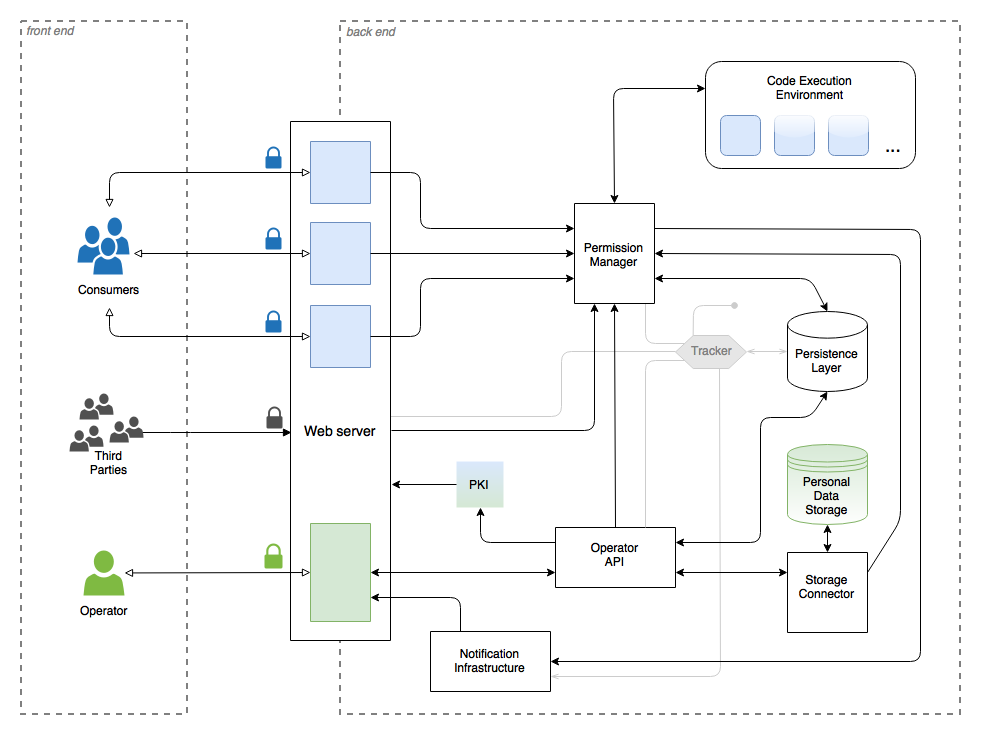
\includegraphics{./assets/figures/pdaas_component-composition_centralized.png}
\caption{PDaaS Architecture, centralized
composition\label{fig:composition-centralized}}
\end{figure}

\begin{figure}
\centering
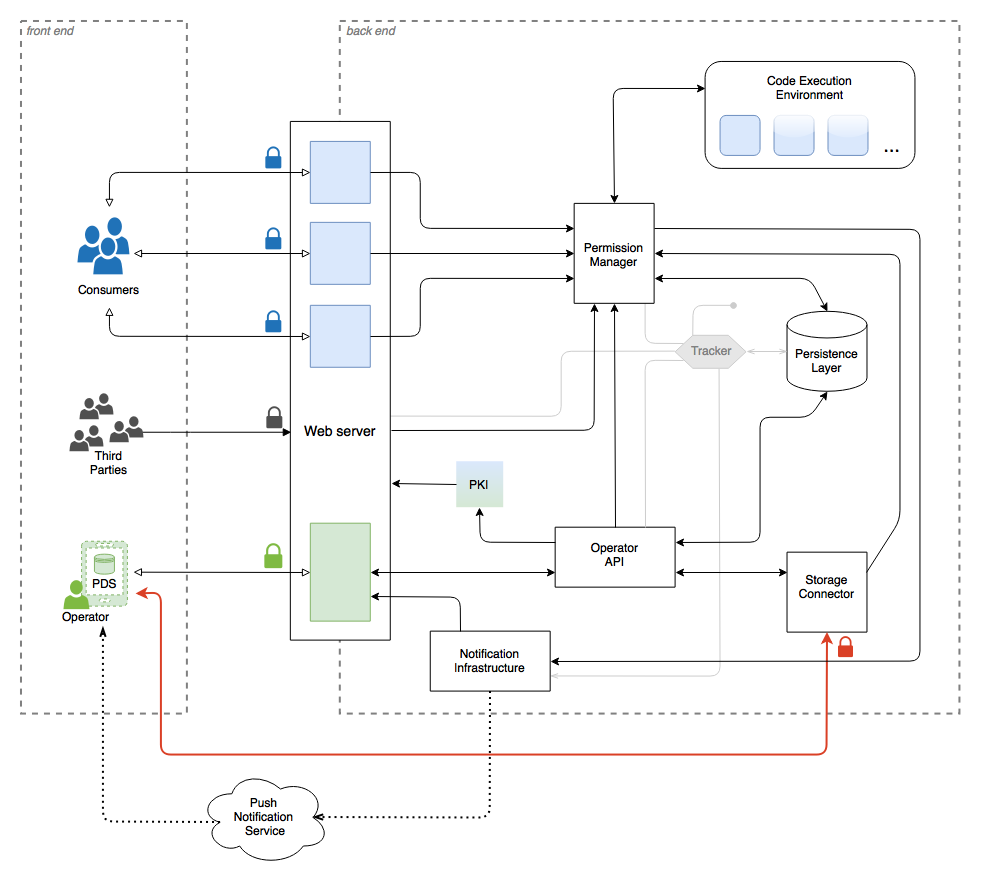
\includegraphics{./assets/figures/pdaas_component-composition_distributed.png}
\caption{PDaaS Architecture, distributed
composition\label{fig:composition-distributed}}
\end{figure}

The main difference between the two compositions is the non-existence of
the mobile platform in the centralized approach (Figure
\ref{fig:composition-centralized}). Although \emph{centralized} only
refers to the components arrangement on a \emph{server} platform,
originally consisting of a single process that contains all components
and is thus is responsible for every task. It is also imaginable that
all server components are note necessarily placed into one server
environment, but being distributed over several virtual machines or
containers, so that they can scale and run more independently. This can
improve \emph{redundancy} as well.

In theory, a possible version of the arrangement would be to move all
components to either the desktop or the mobile platform. This comes
along with some downsides and major issues though, that are far from
trivial to solve. Nevertheless, to not only ensure nearly 100\% uptime
and discovery in a landscape where NAT\footnote{Network Address
  Translation; practice of routing traffic between and through distinct
  networks address spaces by remapping IPs from those different networks
  onto each other (e.g.~by utilizing ports)} and dynamic IPs are still
common practice, for mobile platforms as well as on the desktop, all
components but the user interface need to be implemented natively. From
a \emph{operator's} perspective that would mean, to have all components
at hand and therefore full control over the \emph{PDaaS}. It still would
still raise security concerns, though.

Aside from providing the \emph{operator} with a non-stationary and
instantly accessible interface to her \emph{PDaaS}, involving a
\emph{mobile platform} primarily has the purpose of enabling the
\emph{data subject} to carry all her sensitive data along. This is
considered a major advantage over the centralized approach, were all the
personal data is located in the \emph{`cloud'}. Depending on the
perspective, it can either be seen as a \emph{single source of truth} or
a \emph{single point of failure}. Regardless of that, it introduces the
demand of a backup or some redundancy concept, which has briefly been
touched on in the discussion about database system requirements within
the \protect\hyperlink{data}{section on \emph{data}}. A mobile platform
as part of the system makes it more easier for the data subject to
establish a security concept in which the relation between
\emph{personal data storage} and the rest of the system is much more
liberated, so that all access attempts only happen under full
supervision. It is debatable whether to place the \emph{permission
profiles} in the \emph{persistence layer} among all other domain-related
information, put it into the \emph{personal data storage} too, or define
it as having its own storage component, in order to be flexible in its
placing.

Authenticating \emph{consumers} is performed based on TLS by the web
server and its configured subdomains including their individual keys and
certificates provided by the \emph{PKI}. The \emph{operator}
authentication is done either by the \emph{Operator API} or by the
\emph{web server}, depending on the \emph{web server's} capabilities.
Though, it makes more sense to entrust the \emph{web server} with that
task, because it's the outermost component and it would prevent
unauthorized and potentially malicious requests from getting further
into the system. And since a native front end on a mobile platform is
considered \emph{private} as well, it is reasonable in that case to
change the \emph{operator} authentication from JWT-based to TLS-based
\emph{two-way authentication}, which would otherwise be inconvenient
when using web-based front ends.

If components are placed only on the server and require communication
with each other but are separated into independent processes, then some
inter-process communication need to be established (e.g.~sockets). It is
also conceivable that inter-communication between server components
could just be unidirectional. Approaches like changing configuration
files by writing to the filesystem can therefore be feasible in some
cases. Components that can vary in terms of their platform have to
communicate to other components via \emph{HTTPS}.

The architecture implicitly distinguishes between two different groups
of endpoints. These endpoints that are made available by the \emph{web
server}, which reverse-proxys incoming connections to role-related
(operator* or data consumer) components. Starting from that, this
separation can be driven further by simply encapsulating those
components into services, that are related to one of the roles or used
by both. This basically results in the \emph{web server} communicating
with the two role-grouped services in a bidirectional manner. The group
of endpoints for \emph{data consumers} mainly consists of those through
which \emph{access requests} and \emph{permission requests} are coming
in and the public one, that is used for when consumers apply for
registration. The other one is a small group of endpoints required for
all tools the \emph{operator} might need; from data API or notification
to authentication and web-based user interface. Furthermore, it might be
considerable to partially apply the principles of a RESTful design. At
the same time this makes the API potentially more complicated and
insufficient, since the \emph{Operator API} does not follow the concept
of resources. Instead, it requires a rather functional design, which
makes for example \emph{Remote Procedure Calls} or a
\emph{Publish-Subscribe} pattern more appropriate to use.

Considering the rapid growth of emerging website and applications, which
all require user registration, users are getting tired of creating new
accounts. Hence they tend to reuse their password(s). Providers started
outsourcing that sensitive topic of user management by integrating third
party authentication services, which not only makes that feature almost
effortless to implement, but also leaves the responsibility as well as
the accessibility to those service owners. Whereas users get the benefit
of just using one account for all their apps - a universal key so to
say, but only one exemplar. So the downside here is, in reality only a
handful of third parties
{[}\protect\hyperlink{ref-web_2009-success-of-facebook-connect}{146}{]}
provide those authentication services.\\
OpenID is designed with a very specific type of scenarios in mind,
namely the one just described - bringing decentralization to the market
of authentication services - which differs from the ones addressed by
the \emph{PDaaS}; at least when it comes to \emph{data consumer}
interactions. The \emph{PDaaS} has the ability to become the digital
representation of its \emph{operator}, therefore it can and should also
be used to authenticate that individual against external parties.

\emph{\textbf{Conclusions:}} Considering the amount of effort a
single-platform composition, namely \emph{desktop} or \emph{mobile},
would take to get fully operational with respect to the specification,
it is not only reasonable but also more secure to involve a server
platform with proper security measures, a static IP, and high
availability, even if that server is a local machine connected to the
operator's private network. That said, it is sufficient to start with
the \emph{centralized} approach and as suitable mobile applications
emerge that are supporting major administration features, notifications,
and \emph{personal data storage}, it should be possible to migrate
effortlessly towards the \emph{distributed} approach that brings a
higher level of confidence because all the sensitive personal data is
not on some computer machine somewhere on the internet, but right in the
hands of its owner. By the proposed architecture, all components (or
groups of components) are portable and therefore relocatable among the
suggested platforms; and with the introduced authentication methods for
operators, multiple front ends for the same \emph{PDaaS} are thereby
supported and can be implemented with almost no effort, which, in
return, covers more use cases. As a supplement, an \emph{identity
provider} based on the OpenID standard would fit nicely into the
existing arrangement and does not interfere with the other components.
However, it is beyond the scope of this work to elaborate on this topic.
For now it is stated as a feasible and logical addition to the
\emph{PDaaS}.

\section{Environment and Setup}\label{environment-and-setup}

As stated in the project's \protect\hyperlink{core-principles}{core
principles}, \emph{Open Development} is vital for the project to gain
trust. Interestingly, this has a significant impact on how a
\emph{PDaaS} might be deployed or installed. All its components can just
be grabbed and used as it suits everyone's needs, while respecting their
licenses. Furthermore, enforcing \emph{portability}
(\protect\hyperlink{sa02}{S.A.02}) leads to a more simplified and
independent development process that can be organized in a way so that
the primary division into components can be leveraged.

The range of environment systems for \emph{server} platforms is highly
diverse but the main shares
{[}\protect\hyperlink{ref-web_2017_wikipedia_os-market-share}{147}{]}
belong to either the UNIX or LINUX family, even though almost every
platform is POSIX-compliant.\footnote{Portable Operating System
  Interface; a collection of standards released by the IEEE Computer
  Society to preserve compatibility between operating systems} When it
comes to \emph{mobile} platforms the market is far less diverse. Native
applications are either developed in \emph{Java} (for Google's Android)
or in Swift (for Apple's iOS). Whereas the environment systems have
nearly no relevance for the \emph{desktop}, other then the screen size
and maybe which browser and version the environment system runs. But
that's a situation the user can change if necessary.

As a result, being able to use certain components on a \emph{server}
platform depends on what \emph{server} environment is available and vice
versa. In order to decide what implementation of a component is
suitable, it's crucial to know in which environment that component has
to run. Either way, it is also important not to forget all the
dependencies a component itself might have. Such constraints can be
avoided by abstracting the runtime of those components and either embed
every required software dependency or provide them in separate runtimes,
if possible. Depending on the used technologies, this concept is
commonly known as \emph{virtualization} or \emph{containerization}. It
isolates software by putting them into a so called \emph{container}. But
since those container-wrapped components still have to interact with
each other, they need to be supervised or at least managed. This is done
by an orchestration software, which not only allocates system resources
but is also capable of emulating a whole network infrastructure
(e.g.~DNS, TCP/IP, routing). Thereby, it is utilized to determine how
certain containers (and their contained components) are allowed to
communicate and what resource are accessible from the inside (e.g.
filesystem). This complete abstraction to the surrounding environment
effectively means it's the only dependency the \emph{PDaaS} would have,
regardless of how its components are implemented. They just have to be
\emph{`containerizable'} - by satisfying the
\emph{\protect\hyperlink{def--container}{container image specification}}
{[}\protect\hyperlink{ref-web_oci-spec_image}{115}{]}. This concept can
also be utilized for the
\emph{\protect\hyperlink{supervised-data-access}{supervised code
execution}} (\protect\hyperlink{sa01}{S.A.01}) mentioned before without
any restraints.

Migrating from a server-located \emph{personal data storage} to a
\emph{mobile} based version introduces another challenge. The subsequent
approach is a first and more general solution to that problem.

\emph{NOTICE: it is assumed that a running instance of a }PDaaS* is in
place, the \emph{operator} owns a modern mobile device and on this
device a \emph{PDaaS} mobile application is installed.*

\begin{enumerate}
\def\labelenumi{\arabic{enumi}.}
\item
  After starting the app, the operator needs to establish a connection
  between server and mobile application. Therefore, the operator has to
  scan a QR-Code with the help of that app. The QR-Code is presented to
  the operator within the management tool of the \emph{PDaaS} running in
  a browser. Alternatively, the operator inserts her credentials into a
  form presented by the mobile application.
\item
  After the connection is established, the operator can trigger a
  progress that duplicates all her personal data to the device that has
  just been associated with the \emph{PDaaS}.
\item
  At this point, one of two paths can follow, depending on whether a
  complete write log for the \emph{personal data}
  (\protect\hyperlink{data}{see discussion about backup strategies}
  exists or not.

  \begin{enumerate}
  \def\labelenumii{\alph{enumii})}
  \tightlist
  \item
    If \emph{{[}LOG-EXISTS{]}}, query by query the whole log is obtained
    from the existing storage and is then again executed in
    chronological order by the query language abstraction, starting with
    the oldest. The only difference here is that the target storage, on
    which that query is actually performed on, is located on that newly
    introduced platform.
  \item
    If \emph{{[}LOG-NOT-EXISTS{]}}, the situation is more complicated if
    the database systems are not based on exactly the same technology.
    This would mean additional migration software is required. If both
    database systems provide import and export mechanisms that support
    at least one interoperable data format, the migration software can
    leverage these features simply by exporting all the data and saving
    it to the filesystem. The software then transfers the dump to the
    target environment and triggers the import process. When this is not
    the case, the software not only needs to be aware of both database
    systems and their native query language, it also has to have a
    comprehensive understanding of how their data structuring concepts
    work, in order to reliably transform one into the another. So, to be
    more specific, at first the software has to analyse the structure of
    the source database. Based on this result it might need to perform
    some configuration on the target database before actually obtaining
    the data from there. Received data then needs to be transformed into
    queries that are supported by the target database system. Those
    transformed queries are transferred to the target environment, where
    those incoming queries get executed until all data is migrated.
  \end{enumerate}
\item
  After the duplication process has finished, the operator can decide
  which PDS the \emph{PDaaS} should use to serve \emph{access requests}
  and what should happen with the other storage(s).
\end{enumerate}

To conclude, a migration process like moving \emph{personal data} from
one platform instance to another can be further simplified and robust if
a complete query log would exist. It is also worth mentioning that the
migration process described above is not restricted to exactly this
source or migration direction. As long as target and source are either a
\emph{server} or a \emph{mobile} platform, any variant is imaginable.

\emph{\textbf{Conclusions:}} Installing a \emph{PDaaS} should be
straightforward with the least possible effort being spent for
preparations. Package managers of all popular operating systems should
offer (semi-)automated installations. Additionally, components
themselves and the project as whole have to provide detailed
documentations for various ways of how those parts or the entire system
need to be installed. Alternatively, \emph{data subjects} might be
willing to entrust external third parties with hosting a \emph{PDaaS}
instance for them. In that case, the distributed approach involving a
\emph{mobile} platform might come in handy, so that the actual data is
not stored somewhere beyond their reach. The \emph{PDaaS} as an open
source development encourages anybody who is interested or even wants to
contribute to checkout the source code of the various implementations,
get it to run, and play around with it. Therefore, at least the
components of the \emph{server} platform are required to document what
other software they depend on, so that the target environment can be
prepared properly. Aside from hardware, on which the \emph{PDaaS} needs
to run, the only other requirement is owning an internet domain that is
registered on a public DNS\footnote{Domain Name System; decentralized
  open directory that associates readable (domain) names with IP
  addresses} server and has no subdomains configured yet.

If a component needs to get segregated from its host environment,
\emph{containerization} is the recommended technique since it causes
less overhead compared to \emph{virtualization} and is generally a
lightweight approach. Although additional abstraction might also
introduce new problems instead of solving them.

\section{Attack Scenarios}\label{attack-scenarios}

If only briefly, previous sections already mentioned a few potential
attack types and vulnerabilities of the system, such as
man-in-the-middle attacks that are possible during connection
establishment and data transfer, or session hijacking which can be done
by stealing the JWT used to authenticate privileged entities to the
system. Attack vectors causing those and other scenarios as well as
possible and feasible counter-measures are discussed in detail within
this section.

Initially however, it is to identify what motivation(s) would drive such
attacks. The first and probably the most dangerous one appears to be
\emph{Digital Identity Theft}. Thereby the attacker impersonates the
individual that was originally associated to the system. Then data
consumers, though, have the misleading impression, that everything the
intruder does with the \emph{PDaaS} still happens on behave of the data
owner herself. Such control can be abused for vicious data changes to
harm the physical counterpart or the access can simply be exploited to
unopposedly extract the individual's personal data. The more data the
system contains and the more purposes it serves, the more power can be
gained by controlling it. Those motivations are extrinsically driven by
third parties, whereas intrinsic and mostly unintended damage can be
caused by system or human failure, which may lead, for example, to data
loss or irrecoverable system access.

As the name states, in a man-in-the-middle attack the transferred
content of a communication is intercepted and possibly tampered with,
while the participants not noticing any of that. A common solution here
is to encrypt and sign the content before transferring it. For HTTP
communication this is implemented by the \emph{Transport Layer Security
(TLS)}. The crux here is to move from an unencrypted to an encrypted
connection. This upgrade procedure involves the
\emph{Diffie-Hellman-Key-Exchange} to agree on a pre-shared key and
certification based on \emph{asymmetrical cryptography} for
authentication. The procedure starts i.a. with the server-role
presenting the client-role with its certificate \emph{while the
connection is still insecure}. This is essential, because the connection
is still insecure, a man-in-the-middle attack is possible at that time.
In order to prevent that and to ensure the trustworthiness of that
certificate, the client has to verify the certificate. This is done by
using an installed certificate from a trustful public CA, that has
issued and therefore trusted the server's certificate, to examine its
chain of trust. But since HTTPS connections between data consumers and
the system rather use certificates that are issued by the system itself
instead of relying on CA-certified certificates, there is no chain of
commonly trusted entities, that can verify the presented certificates.
So in order to still trust those certificates, even though they are sent
on a insecure channel during the connection establishment, they have to
be handed over in private sometime before. This is defined in the
registration process, where the consumer either presents a QR-Code
served via publicly certified HTTPS, which he is responsible for but can
easily verified by the data subject, or submits the registration request
including the CSR to a URL provided by the data subject that is also
reachable only by publicly certified HTTPS. The server then issues the
certificate and sends it - alongside with its own certificate - back to
the consumer via publicly certified HTTPS, too. The consumer is able to
trust the server certificate and can even pin it to detect fictitious
certificates he might get presented with. This approach enables not only
confidentiality and integrity of the data exchanged between consumer and
data subject, but by enforcing \emph{two-way authentication}
authenticity of the respective opposite is provides to both parties as
well. While other HTTP connections via TLS may still rely on
certificates signed by publicly trusted CAs, regular key change and
certificate renewal has therefor to be ensured.

Another aspect of the system, that could be vulnerable to certain
attacks, is the authentication mechanism used by the data subject to log
into her management tool. A JSON Web Token, also containing all session
information, serves as the key. As mentioned before, such connections
are forced to be established only by TLS. So from this perspective the
JWT is no less or more secure than any other type of credentials.
Though, this doesn't prevent the token from being usable to the attacker
once it is stolen. A short expiration date, equally to a session
timeout, and token invalidation cycle, which is the same as forced
logout, can reduce the potential harm an incident like this may cause.
Furthermore the integration of 2-factor authentication hardens the
authentication procedure. But in order to not introduce another
dependency, namely an external service providing such functionality,
2-factor authentication is only supported, when a mobile device is
associated to the \emph{PDaaS}. Further precautions can be taken by
preventing attackers from getting in the near of such token, referring
to \emph{cross-site scripting (XSS)}, to which web-based graphical
interfaces are vulnerable to. Approaching this issue means to abandon
external resources providing parts of the interface and instead store
all content on the server platform and serve it with the system's own
web server. Even if that means an increased load time caused by the
browser constrains of how content is loaded, which isn't an issue in
HTTPS/2 anymore.

The approach of running consumer-provided programs locally in order to
prevent personal data from leaving the system represents a key part in
this work, but it also raises major security concerns. To address those
concerns such a program is executed in an application container, which
encapsulates the runtime from the host environment and allows to
restrict resource access, such as network, filesystem or computing
power, to the required minimum. This concept, previously introduced as
\emph{Supervised Code Execution} forms a containment layer preventing
security breaches towards the host environment, which ultimately means a
great security enhancement. Nevertheless, it makes involved components
and dependencies vulnerable for almost any security flaw that they might
carry in. Therefore it is vital to keep all related software up to date,
which probably means enabling automated update mechanisms. That again
introduces yet another type of attack vectors, which can be depressed by
only using signed and trusted software and resources.

When it comes to personal data, existing social networks and other great
platforms, founded on user-generated content have already become de
facto data silos, and thus a single point of failure. A more
decentralized approach, for example the here proposed concept would
result in, diminishes the impact of potential security breaches, those
platforms may experience. While from an global perspective this can be
valued as a step in the right direction, from the perspective of a data
subject instead, a \emph{PDaaS} instance still represents a single point
of failure as well. But in order to provide most control over the own
personal data, this design choice appears to be the logical consequence.
Besides that, several system components are highly portable, so that
more sensitive parts, like the \emph{Personal Data Store}, can be
relocated away from the server platform into the data owner's mobile
device. In this case, for example a JWT issued by the \emph{PSD} can be
used to authenticate the access to personal data.

However, those measures are still no guarantee for a comprehensive
security protection. The only way is to continuously improve the system
and provide mechanisms to securely recover from any type of incident.
Not least that's why a complete open (source) development is enforced
from the start, because vulnerabilities can easy be disclosed and hence
addressed immediately.

\emph{\textbf{Conclusions:}} Securing data transport and storage are the
two pivotal aspects to focus on. Choosing self-singed certificates over
publicly trusted CAs in order to not only encrypt but also reasonably
authenticate the consumer-system communication requires to make sure
that the preliminary transfer of the certificates is not compromised, so
that both parties can safely rely on them. Settings for any
cryptographic procedure regarding their expense have to be chosen in
favour of increasing the level of security instead of reducing resources
and cost. The general mindset for this project is to rather utilize long
proven libraries and technologies instead of using own implementations
for cryptographic concepts and algorithms. Nevertheless, ongoing
reviewing and re-evaluation of those dependencies as well as the
software itself is mandatory.

As a future enhancement it is planned to integrate an \emph{intrusion
detection system} into the server platform's host environment, even
though all server components are recommended to be encapsulated by
containers. Monitoring transactions and events on the application-level
is already part of the system architecture, facilitated by the
\emph{Tracker} component. Furthermore it is considered to apply full
storage encryption to the \emph{Personal Data Storage}, which would
result in major security improvements. Therefore, when the personal data
is located on the server, it should stay secure, even if the system is
compromised. In return, the system might lose convenience in user
interaction. It essentially comes down to an act of balance between
security and convenience. Not much security measure or mechanism can be
simplified or abstracted while not violating other (general) values at
the same time. Key is to find the right compromise for the right motive.

\section{User Interfaces}\label{user-interfaces}

Designing graphical user interfaces is beyond the scope of this work and
the \emph{PDaaS} specification as well. Nevertheless this section shall
be understood as a collection of proposed ideas addressing the questions
of what types of user interfaces the \emph{PDaaS} should provide and
which features they might need to support.

The most notable characteristic used to distinguish user interfaces from
each other are those interfaces that are visible and the ones that
arn't. For example a \emph{graphical user interface (GUI)}, composed of
visually separated areas with a certain semantic and assembled with
meaningful objects on which the user can physically act, for example by
touching them. The interface then reacts on those actions by changing
its appearance. In this way the user can recognize and comprehend her
actions. Whereas non-graphical user interfaces don't provide the user
with objects or surfaces to interact with. Instead, the primary medium
is text, regardless if it's human-readable or not. But \emph{command
line interfaces (CLI)}, available mainly in command line environments or
shells, still provide a certain level of interactivity. A running
program can pause in order to prompt the user with an input request. If
an input is made and submitted, the program then proceeds. The group of
interfaces whose interactions can be programed and thereby fully
automated can be called \emph{application programming interfaces (API)}.
Depending on the transport technologies, it's not unusual that
\emph{API} interactions consist of just one action causing one reaction.
Non-graphical interfaces enable interactions on a lower level. Even
though they provide more functionality and can be more time efficient,
they are more rudimentary and often less secure. While \emph{GUIs} are
normally meant for end users to interact with applications on a more
sophisticated level, \emph{CLIs} are used during development, for
automation, or for server environment administration; probably remotely
since they are typically headless. Whereas \emph{APIs}, documented by
their providers, enable software developers to program automated
requests against those interfaces.

Table \ref{tbl:ui-features} provides a list of features and associates
the different types of user interfaces mentioned before, which indicates
if they should be supported by a certain type. It is notable that the
\emph{GUI} provides the \emph{operator} with a powerful tool Hence it
requires reliable protection mechanisms (see
\protect\hyperlink{authentication}{Authentication}). Whereas \emph{API}
capabilities are very limited, because it's the one interface that the
\emph{PDaaS} exposes to third parties.

\begin{longtable}[]{@{}lccc@{}}
\caption{Features that should be supported by the given user interfaces
\label{tbl:ui-features}}\tabularnewline
\toprule
Feature & GUI & CLI & API\tabularnewline
\midrule
\endfirsthead
\toprule
Feature & GUI & CLI & API\tabularnewline
\midrule
\endhead
manage permission profiles (\protect\hyperlink{pviu03}{P.VIU.03}) &
\textbf{X} & - & \textbf{X}\tabularnewline
view access history (\protect\hyperlink{pviu04}{P.VIU.04}) & \textbf{X}
& \textbf{X} & -\tabularnewline
register consumer & \textbf{X} & \textbf{X} & -\tabularnewline
add new front end & \textbf{X} & - & -\tabularnewline
authenticate operator & \textbf{X} & - & -\tabularnewline
migrate personal data & \textbf{X} & \textbf{X} & -\tabularnewline
review permission requests (\protect\hyperlink{pi04}{P.I.04}) &
\textbf{X} & - & -\tabularnewline
create \& maintain templates (\protect\hyperlink{pi05}{P.I.05}) &
\textbf{X} & - & -\tabularnewline
adjust precision of data (\protect\hyperlink{pi06}{P.I.06}) & \textbf{X}
& - & \textbf{X}\tabularnewline
introduce new data structs & \textbf{X} & - & \textbf{X}\tabularnewline
configure \emph{PDaaS} & \textbf{X} & - & -\tabularnewline
import personal data & \textbf{X} & - & \textbf{X}\tabularnewline
read/access personal data & \textbf{X} & \textbf{X} &
\textbf{X}\tabularnewline
manipulate personal data & \textbf{X} & \textbf{X} & -\tabularnewline
run supervised code execution & - & \textbf{X} &
\textbf{X}\tabularnewline
\bottomrule
\end{longtable}

The architectural design includes \emph{desktop} and \emph{mobile}
platforms. While prioritizing a web-based \emph{GUI}, the management
tool for the \emph{operator} also needs to be natively implemented for
common mobile systems (\protect\hyperlink{pviu02}{P.VIU.02}); in this
case Android and iOS. This enables real-time notifications
(\protect\hyperlink{pi03}{P.I.03}, \protect\hyperlink{pb02}{P.B.02}) on
mobile platforms, whereas the same feature is added to \emph{desktop}
platforms by providing WebSocket-based connections. Since screen sizes
can vary - in particular on \emph{mobile} platforms - the \emph{GUI} is
required to be highly responsive and has to adapt
(\protect\hyperlink{pviu01}{P.VIU.01}) to various screen sizes. Given
the capabilities of the management tool, an inaccurate or error-prone
rendered \emph{GUI} can quickly cause unintended incidents. Thus, the
main focus must be to ensure a very robust and low-latency interface
rendering.

Known challenges for the \emph{GUI} design are primarily to develop very
efficient, but also fun to use interfaces for reviewing \emph{consumer
registrations} and \emph{permission requests}. The latter can become
especially hard to solve because of the problem of how to display
graph-based and nested data structures in such a way that reviewing and
also manipulating them is easy, even on the small screen of a mobile
phone? One approach could be to utilize the \emph{accordion} pattern
{[}\protect\hyperlink{ref-web_2016_wikipedia_accordion-gui}{148}{]} for
edges and start nesting them in order to represent subsequent data
structure. The interaction then might look like tree-structured
navigation; moving alongside relations just by expanding and folding in
data items.

Since other parts of the system have to provide the mechanisms for
increasing or reducing the precision of data due to privacy protection,
the challenge here is to find the right design concepts for the data
subject to facilitate those adjustments. Precision adjustments can be
achieved by either changing the sampling rate in a dataset containing a
series of data items, or by rounding values to a certain extent.
Examples are cutting fractional digits of the latitude and longitude
values in a position, or removing all position information obtained
between every quarter from a full day tracking period. Whether data
subjects can choose from an abstracted precision grading (e.g.
\emph{high}, \emph{mid}, and \emph{low}) or they set specific type or
unit related filter mechanisms, configurable defaults on a system-wide
level should be provided by \emph{GUIs} in any case. The following data
types are supposedly vulnerable to compromising privacy, thus proposed
to support precision adjustments: \emph{Date} (time), any kind of
absolute measurements, sets containing data series, and position
information, as mentioned before.

\emph{\textbf{Conclusions:}} The most important aspect, when interacting
with something or someone, is being provided with feedback. An action
typically causes - and is therefore \emph{expected} to cause - a
reaction. The result is an interaction, unless no reaction occurred.

The discussion above outlines the relevance of those interactions for
the \emph{PDaaS}. Thus, for users and other software to interact with
the \emph{PDaaS} interfaces are mandatory. Primary characteristics of
those interfaces are complete functionality, security precautions and
restrictions, as well as comprehensive documentation. Visual user
interfaces also need to provide reliable and adaptive rendering, a
consistent and encouraging interaction design. \emph{GUIs} need to be
provided for all \emph{desktop} and \emph{mobile} platforms, primarily
to provide an efficient user experience for the operator. The operator
is the only role with permissions to access a \emph{GUI}. Components on
the \emph{server} platform should provide \emph{CLIs}, at least when no
other technical option exist to interact with them. Also accessing the
database from command line could be appreciated at some point. APIs are
mostly meant for data consumers to interact with the \emph{PDaaS}, and
perhaps for automated data contribution (based on \emph{operator} role;
e.g.~browser plugin). \emph{Desktop} platforms might use those
\emph{APIs} as well. In any case, \emph{APIs} must be separated
according to the \emph{roles}.

These are all vital characteristics whose details need to be addressed
by the \emph{specification}. Their implementation details are not the
concern of this specification, as long as every stated requirement is
being acknowledged.

\chapter{\texorpdfstring{Specification
\emph{(Draft)}}{Specification (Draft)}}\label{specification-draft}

\hfill~ \emph{Version 0.1.0}

This chapter holds the first draft of what might become an open
specification. As for now it has therefore no claim of completeness,
continuity or accuracy. Frequent changes are to be expected. The
contents is based on and a result of all previous discussions and
developed solutions. Hence, parts of the contents can be expected to
reoccur.

\subsection*{Introduction}\label{introduction-1}
\addcontentsline{toc}{subsection}{Introduction}

This specification describes a system with the purpose of controlling
the personal data of a single entity. By `entity' it is primarily
referred to a person, an individual. This individual manages all data
relating to her in an online platform, operated by her, which exposes a
service making those data selectively accessible to third parties that
might have an interest in them. Meanwhile the system tries to ensure
that not personal data ever leaves the system. The overall flexibility
and portability of the system enables the individual to store her data
for example on a mobile phone so that she is able to carry all her
personal data along while the accessibility of the data is ensured at
all time.

\subsection*{Notation and Conventions}\label{notation-and-conventions}
\addcontentsline{toc}{subsection}{Notation and Conventions}

The requirements notation used in this document originates in the
\href{https://tools.ietf.org/html/rfc2119}{RFC 2119} and shall be
interpreted as described in there. This applies to the following
keywords, recognizable through capital letters: MUST, MUST NOT,
REQUIRED, SHALL, SHALL NOT, SHOULD, SHOULD NOT, RECOMMENDED, MAY and
OPTIONAL.

Values and words presented in a \texttt{fixed-width\ font} need to be
understood as names and must therefore be used as is. If one of those
starts with a \texttt{\$} (Dollar) character, a variable is indicated,
which means for implementations, this variable has to be replaced with
the actual value.

Lists that are numbered outline its given order, which must therefore be
followed. Lists that start with a character (upper or lower case) have
no claim to its order. Their items are inclusive (logical \emph{and}),
while bullet list items are exclusive (logical \emph{or}).

\subsection*{Terminology}\label{terminology}
\addcontentsline{toc}{subsection}{Terminology}

\begin{description}
\item[\protect\hypertarget{spec_term_system}{}{(The) System}:]
refers to either the overall concept or the implementation of this
specification
\item[\protect\hypertarget{spec_term_platform}{}{Platform}:]
combination of environment capabilities and common role characteristics,
which can be inherited form its hardware/device properties; possible
values: \emph{desktop}, \emph{server}, \emph{mobile}
\item[\protect\hypertarget{spec_term_component}{}{Component}:]
independent piece of software that is part of the system and might be
capable of running on different platforms, but not at the same time
though; serves a unique purpose within the system
\item[\protect\hypertarget{spec_term_operator}{}{Operator}:]
data subject and owner, not necessarily provider or host though;
individual, represented by the system and whose personal data can be
accessed through the system; also referred to as \emph{data controller},
\emph{data subject} or \emph{data owner}
\item[\protect\hypertarget{spec_term_third-party}{}{Third Party}:]
external entity or vendor, who is yet to become registered as a
\emph{consumer} to the system
\item[\protect\hypertarget{spec_term_consumer}{}{(Data) Consumer}:]
external entity or vendor, who has registered to the system and is
therefore permitted to request access to data or even to access data
hold by the system
\item[\protect\hypertarget{spec_term_contributor}{}{(Data)
Contributor}:]
external entity, that is authorized by the \emph{operator} to obtain and
push personal data of hers into the system
\item[\protect\hypertarget{spec_term_personal-data}{}{Personal Data}:]
data, relates to the \emph{operator}, that is contained in the system
and selectively permitted to get accessed by consumes
\item[\protect\hypertarget{spec_term_data-broker}{}{Data Broker}:]
entity with commercial interests in collecting, aggregating and
analyzing personal data from any possible resource in order to combine
and enrich those, to license the result to other entities
\item[\protect\hypertarget{spec_term_endpoint}{}{Endpoint}:]
dedicated entry for a specific \emph{data consumer} to communicate with
the system (e.g.~access personal data)
\item[\protect\hypertarget{spec_term_permission-profile}{}{Permission
Profile}:]
set of access rules and configurations tied to an \emph{endpoint},
defining e.g.~how long or often and what personal data is accessible by
a related \emph{data consumer}
\item[\protect\hypertarget{spec_term_access-type}{}{Access Type}:]
defines the method of how the access to personal data is provided
\end{description}

\section{Overview}\label{overview}

The overall purpose of this specification is to provide detailed
instructions for building a web service that, on the one hand,
encourages an individual to manage and maintain all the data relating to
her in one place, and on the other hand, enables third parties to access
such data if they are permitted by the individual to do so, preferably
through supervised code execution instead of just handing over the raw
data items. The result is a one-to-many relation between the data owner
- the individual - and all those who might require some data to, for
example, process a purchase initiated by the operator or make a proper
decision on her medical treatment.

The system architecture is designed with flexibility and portability in
mind while still preserving simplicity and security. The result supports
running some components on different platforms in a distributed way.
Therefore the operator is able to operate the system while being on the
move and can literally carry all her personal data along.

The design of this specification tries to leverage as many existing
standards and open technologies as possible for every aspect and
component. By recognizing common practices, its implementation and
integration can be made as effortless as possible.

\subsection{Key Features}\label{key-features}

\textbf{Perspective: \emph{Operator}}

\begin{itemize}
\tightlist
\item
  full control over the flow of personal data
\item
  maintain all personal data in one place
\item
  real-time information and notification
\item
  taking her personal data with her
\item
  collect and analyze her own personal data
\item
  trust through open development and open source
\item
  commercialize data access on her own
\end{itemize}

\textbf{Perspective: \emph{Consumers}}

\begin{itemize}
\tightlist
\item
  reliable single source of latest data about an individual
\item
  access only those data that are actually required and thus reduce
  `noise'
\item
  access data that have never been collectible before
\item
  distributed computing
\end{itemize}

\subsection{\texorpdfstring{Scenarios
\emph{(Excerpt)}}{Scenarios (Excerpt)}}\label{scenarios-excerpt}

\paragraph{Online Purchase}\label{online-purchase}

In order to proceed with checkout, a shop requires some personal data
from the user, such as shipping address, email, and payment information.
Either the shop is already a data consumer, then it would access the
system in the background to check if any data has changed, or the shop
has to register as a consumer first. After the registration process has
been initiated, if needed, the user is forwarded to complete the
checkout. After reviewing the registration and the data that are
attempted to be accessed, the user is informed via email that the order
has been processed and the shipment has started.

\paragraph{Social Network}\label{social-network}

Instead of storing personal data by itself, a social network, after
registering and being permitted to, can request and display data about a
user whenever other users try to access them. Created content such as
posts, comments, images, or videos can be stored in the system as well.
The social network then just holds references to all the content so that
it can obtain and forward information on how to request those data, for
example, with a one-time url.

\paragraph{Apply for a Loan}\label{apply-for-a-loan}

The data that credit institutes take into account when deciding on
creditworthiness of an individual can be directly accessed through the
system; instead of gathering and acquiring them from all sorts of
resources, including filled out forms from applicants. The credit
institute takes out the part of the computation that is responsible for
those calculations and hands it over to the system after it is permitted
by the operator to do so. The system invokes that computation with the
required data items and sends the result back to the credit institute.

\paragraph{Browser History}\label{browser-history}

A browser plugin, which is connected to the service, keeps track of
every called URL. Those data, collected by the operator, can not only be
reviewed and analyzed by herself, but also be made available to data
consumers.

\paragraph{Movement Profile}\label{movement-profile}

Instead of letting third party apps keep track of an individual's daily
movements (e.g.~fitness app), an app that is associated with the system,
obtains and pushes those location data directly into it. If a third
party is now interested in those data, it can apply and eventually get
permitted to access those movement data, but at a resolution the data
subject is comfortable with.

\subsection{Architectural Overview}\label{architectural-overview}

The architecture design (see Fig. \ref{fig:spec_arch_simplifier})
defines three different platforms where components of the system could
run. While \emph{desktop} and \emph{mobile} platforms are primarily
meant to serve as the front end of the system and to present the
operator with GUIs, the \emph{mobile} platform in particular might host
the \emph{Personal Data Storage}. However, that data storage can be
located on any platform. This is enabled by abstracting the storage
through the \emph{Storage Connector} on the \emph{server} platform.

That \emph{server} platform also provides an external API for accessing
personal data. Incoming requests from third parties and consumers are
then processed by the \emph{Permission Manager}, which i.a. decides if
and how data can be accessed. For every consumer a dedicated exposed
endpoint is provided that consists of a subdomain (e.g.
\texttt{CONSUMER\_ID.system.tld}). Other components are i.a. a
\emph{Code Execution Environment}, a \emph{PKI} that provides and issues
certificates and key-pairs to facilitate authentication at the
endpoints. The \emph{Persistence Layer} is represented by potentially
multiple technologies, such as databases or filesystem. A
\emph{Notification Infrastructure} streamlines the different ways and
technologies to notify the operator about certain events (e.g.~system
receives new registration). Probably one of the most important
components is the \emph{Operator API}, through which the operator i.a.
is able to configure the system or manage permissions and the API is
granted read/write permissions at the \emph{Storage Connector}. The
\emph{Operator API} MAY partially be designed RESTful, but accessing
data MUST solely consist of the query language provided by
\emph{GraphQL}.

\begin{figure}
\centering
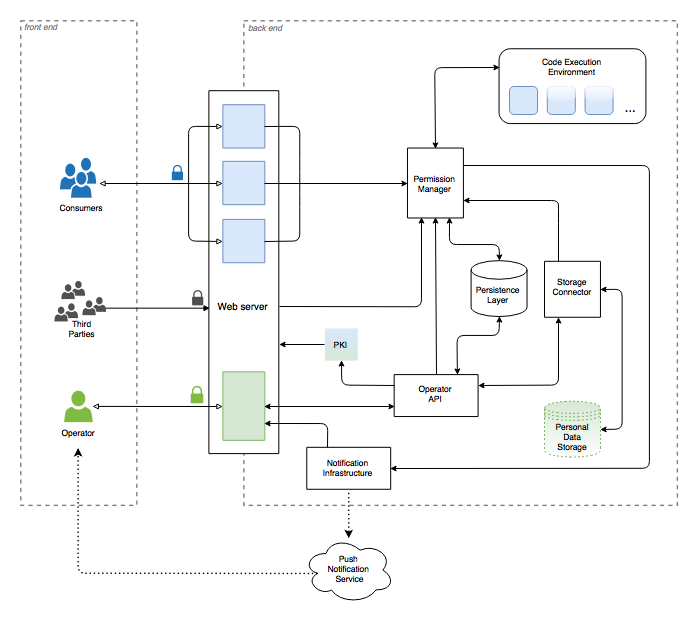
\includegraphics[width=12.00000cm]{./assets/figures/spec_arch_simplifierd.png}
\caption{System Architecture,
simplified\label{fig:spec_arch_simplifier}}
\end{figure}

\subsection{General Process
Description}\label{general-process-description}

\begin{enumerate}
\def\labelenumi{\arabic{enumi}.}
\setcounter{enumi}{-1}
\item
  \emph{Prerequisites: the data subject has an up-and-running system;
  existing third party aims to access personal data on the system}
\item
  Third party has to register at the system to become a data consumer,
  therefore it has to provide certain information to the operator either
  via QR-Code, which the operator can scans, or by submitting those
  information to a unique URL that is generated upfront and provided by
  the operator to the third party.
\item
  Operator reviews the registration. On a positive outcome a new
  endpoint gets defined and, depending on the content of the
  registration request, a permission profile is optionally created and
  configured by the operator. If the outcome instead is negative, an
  error message is prepared. In any case, the third party is then
  informed about the outcome via callback URL and optionally provided
  with additional information that is required for further interactions.
\item
  After the consumer has set up a client according to the documentation
  and the information he has been provided with, and after he
  successfully authenticates to the system, he then submits a query to
  the dedicated endpoint.
\item
  The incoming query is parsed and validated against all associated
  \emph{permission profiles}. If the query passes, the request is
  processed according to configurations and depending on the determined
  \emph{access type} (e.g.~supervised code execution or plain
  forwarding). The response to the consumer either contains information
  about when and where the result can be obtained, or the actual result
  is included directly.
\item
  Finally, the query result is returned to the consumer, either directly
  or self-obtained later on.
\end{enumerate}

\subsection{Relations}\label{relations}

\paragraph{consumer:endpoint {[}1:1{]}}\label{consumerendpoint-11}

one entity (consumer) relates to one access point (endpoint),
exclusively accessible and authenticated by TLS-based \emph{two-way
authentication}

\paragraph{endpoint:permission-profile
{[}1:n{]}}\label{endpointpermission-profile-1n}

zero or more \emph{permission profiles} are associated to one
\emph{endpoint} and are therefore responsible and included in the query
validation procedure

\paragraph{storage-connector:personal-data-storage
{[}1:n{]}}\label{storage-connectorpersonal-data-storage-1n}

the \emph{Storage Connector} MUST be able to access at least one or more
\emph{Personal Data Storage}, regardless of its location (platform)

\subsection{Depending Technologies and
Standards}\label{depending-technologies-and-standards}

\begin{enumerate}
\def\labelenumi{\alph{enumi})}
\tightlist
\item
  HTTP (\href{https://tools.ietf.org/html/rfc2616}{RFC 2616},
  \href{https://tools.ietf.org/html/rfc7540}{RFC 7540})
\item
  TLS (\href{https://tools.ietf.org/html/rfc5246}{RFC 5246}
\item
  WebSockets (\href{https://tools.ietf.org/html/rfc6455}{RFC 6455})
\item
  JSON
  (\href{http://www.ecma-international.org/publications/files/ECMA-ST/ECMA-404.pdf}{ECMA-404})
\item
  JWT (\href{https://tools.ietf.org/html/rfc7519}{RFC 7519},
  \href{https://tools.ietf.org/html/rfc7515}{RFC 7515},
  \href{https://tools.ietf.org/html/rfc7516\%7D}{RFC 7516})
\item
  GraphQL (\href{https://facebook.github.io/graphql/}{Working Draft --
  October 2016})
\item
  Open Container Specifications (by Open Container Initiative)

  \begin{itemize}
  \tightlist
  \item
    \href{https://github.com/opencontainers/image-spec/blob/master/spec.md}{image}
  \item
    \href{https://github.com/opencontainers/runtime-spec/blob/master/spec.md}{runtime}
  \end{itemize}
\item
  X.509 (\href{https://tools.ietf.org/html/rfc5280}{RFC 5280}
\item
  ACME (\href{https://ietf-wg-acme.github.io/acme/}{Draft 05})
\end{enumerate}

\begin{itemize}
\tightlist
\item
  document-based database systems
\item
  browser-supported technologies (HTML, CSS, JavaScript)
\item
  Swift, Java
\end{itemize}

\subsection{Prerequisites}\label{prerequisites}

\begin{enumerate}
\def\labelenumi{\alph{enumi})}
\tightlist
\item
  DNS-registered Domain
\item
  publicly reachable server (e.g public IP or dynamic DNS)
\item
  {[}OPTIONAL{]} mobile device
\end{enumerate}

\section{Components}\label{components}

\paragraph{Web server}\label{web-server-1}

an interface to (or proxy for) server components

\begin{enumerate}
\def\labelenumi{\alph{enumi})}
\tightlist
\item
  process incoming traffic originating by operator, consumer, and third
  parties
\item
  all other server components are reachable only through this component
\item
  serve web-based front ends
\item
  perform all TLS-based authentications
\item
  perform load balancing, if necessary
\item
  pass through notification for web-based Management Tools that are
  connected via Web Sockets
\item
  rule-based traffic management leveraging network characteristics and
  similar
\end{enumerate}

\paragraph{\texorpdfstring{Permission Manager
\emph{(PM)}}{Permission Manager (PM)}}\label{permission-manager-pm}

processes incoming requests from third parties or consumers

\begin{enumerate}
\def\labelenumi{\alph{enumi})}
\tightlist
\item
  parse requests and proceed accordingly
\item
  examine and check queries that are aiming to access personal data
\item
  queue requests if further processing is blocked
\item
  notify operator about new registration attempts
\item
  create and manage permission profiles
\item
  read personal data through \emph{Storage Connector}
\item
  delegate supervised code execution and obtain result
\end{enumerate}

\paragraph{Key Infrastructure (PKI)}\label{key-infrastructure-pki}

provides the web server with keys and issues certificates

\begin{enumerate}
\def\labelenumi{\alph{enumi})}
\tightlist
\item
  issue certificate based on CSR provided by third party
\item
  create and self-sign a system key-pair
\item
  create and sign key-pairs for every endpoint
\item
  maintain certificates and their validity (recurring renewal) issued by
  trusted public CAs
\item
  create new Diffie-Hellman groups
\end{enumerate}

\paragraph{Storage Connector}\label{storage-connector-1}

abstracts the \emph{Personal Data Storage} and facilitates read, write,
changelog and permissions

\begin{enumerate}
\def\labelenumi{\alph{enumi})}
\tightlist
\item
  basic access management
\item
  connect to the PDS
\item
  validate query according to the abstracted query language
\item
  query personal data
\item
  keep track of all changes
\item
  provide migration and backup possibilities
\end{enumerate}

\paragraph{\texorpdfstring{Personal Data Storage
\emph{(PDS)}}{Personal Data Storage (PDS)}}\label{personal-data-storage-pds}

a database system where the personal data is actually stored

\begin{enumerate}
\def\labelenumi{\alph{enumi})}
\tightlist
\item
  can be located on any platform
\item
  capable of translating the abstract query language into
  domain-specific query languages required by the supported database
  systems
\item
  add, change, remove personal data
\item
  provide translations for common operations (filter, sort, aggregate)
\item
  store change history
\item
  store binary data
\end{enumerate}

\paragraph{Operator API}\label{operator-api-1}

provides all functionalities an operator must be capable of

\begin{enumerate}
\def\labelenumi{\alph{enumi})}
\tightlist
\item
  perform all JWT-based authentications
\item
  read and write personal data through \emph{Storage Connector}
\item
  configure, maintain, and monitor system
\item
  provide access history
\item
  manage data structs
\item
  can control \emph{Permission Manager}
\item
  administrate restricted access for \emph{data contributors}
\end{enumerate}

\paragraph{\texorpdfstring{Code Execution Environment
\emph{(CEE)}}{Code Execution Environment (CEE)}}\label{code-execution-environment-cee}

provides isolated runtime (sandbox) for supervised code execution

\begin{enumerate}
\def\labelenumi{\alph{enumi})}
\tightlist
\item
  invoke software provided by data consumers with required data items
\item
  restrict access to the host environment
\item
  provision runtimes
\item
  perform test runs and code review
\item
  monitor runtime during invocation
\item
  hand results back to \emph{Permission Manager}
\item
  archive software in \emph{Persistence Layer}
\end{enumerate}

\paragraph{Tracker}\label{tracker-1}

logs events and transactions occurring in the system

\begin{enumerate}
\def\labelenumi{\alph{enumi})}
\tightlist
\item
  track states of ongoing access requests
\item
  provide data for monitoring and system analytics
\item
  log access history
\item
  pattern recognition and anomaly detection
\end{enumerate}

\paragraph{\texorpdfstring{Persistence Layer
\emph{(PL)}}{Persistence Layer (PL)}}\label{persistence-layer-pl}

combines multiple technologies to represent and hold the current system
state

\begin{enumerate}
\def\labelenumi{\alph{enumi})}
\tightlist
\item
  store:

  \begin{itemize}
  \tightlist
  \item
    system related data
  \item
    component configuration
  \item
    data provided by the \emph{Tracker}
  \item
    permission profiles
  \item
    tokens
  \end{itemize}
\item
  filesystem access
\item
  hold keys and certificates
\item
  cache certain runtime data
\end{enumerate}

\paragraph{Notification
Infrastructure}\label{notification-infrastructure-1}

a unified facility for server components to distribute notifications to
multiple front ends

\begin{enumerate}
\def\labelenumi{\alph{enumi})}
\tightlist
\item
  notify operator about pending approval or review
\item
  support native mobile notifications through connected Push
  Notification Service
\item
  is able to send email
\end{enumerate}

\paragraph{Data Contributor}\label{data-contributor}

an authorized entity, typically software, that sends personal data into
the system

\begin{enumerate}
\def\labelenumi{\alph{enumi})}
\tightlist
\item
  MUST be explicitly authorized by the operator
\item
  data structure and format MUST be known by the system
\end{enumerate}

\paragraph{Management Tool (and other GUIs used by the
operator)}\label{management-tool-and-other-guis-used-by-the-operator}

a graphical user interface, available for mobile and desktop platforms,
accessible only by the operator to control the system

\begin{enumerate}
\def\labelenumi{\alph{enumi})}
\tightlist
\item
  based on either web technologies or native technologies that are
  supported by mobile platforms
\item
  offer all relevant features provided by the Operator API
\item
  scan third party registrations via QR-Codes or generate URL to submit
  registration
\end{enumerate}

\section{Security}\label{security}

The following measures are required in order to improve upon and ensure
a sufficient level of security. Configurations mentioned below MAY
change due to issues or vulnerabilities emerging in the future.

\subsection{Transport}\label{transport}

All communication from and towards the system as well as internal
communication between components located on different platforms MUST be
established with \emph{HTTP over TLS}. Thus, external third parties are
only allowed to communicate with the system on port \texttt{443},
whereas internal communication runs through port \texttt{4223}. Port
\texttt{80} MUST return HTTP Error \texttt{403\ Forbidden} and all other
ports SHOULD be dropped or blocked.

The key-pair, used in TLS to agree on a mutual symmetric key, MUST be
based on either the \emph{RSA} or \emph{DSA} cipher suite, although
\emph{RSA} SHOULD be preferred. All created keys MUST have a length of
at least \texttt{4096} bits. Those ciphers for TLS, that support
\emph{Perfect Forward Secrecy} SHOULD be preferred, but ciphers that are
not supported by \texttt{TLSv1.2} MUST be avoided. All endpoints and
other dedicated entry points MUST provide their own generated
Diffie-Hellman groups with a minimal length of \texttt{4096} bits.

For web-based GUIs \emph{TLS session resumption} SHOULD be activated,
but for \emph{endpoints} it MUST be deactivated. Web-based GUIs MUST NOT
depend on external resources. All involved assets MUST be stored in the
system and thus get served by the \emph{web server}. This required
behaviour is enforced by setting the \emph{Content Security Policy
(CSP)} in HTTP headers, which also eliminates the risk of Cross-site
scripting (XSS) attacks. The \emph{web server} MUST facilitate a web
socket connection for web-based GUIs. If a browser does not support this
natively, a fallback SHALL be provided by the GUI. Furthermore, those
GUIs SHOULD be served with HTTP/2.

The subsequent examples show two Nginx configurations for the \emph{web
server} component, implementing the specifications from above.

\textbf{\protect\hypertarget{spec_code-01_nginx-config-web-gui}{}{Code
01: web server configuration for a web-based GUI (excerpt)}:}

\begin{Shaded}
\begin{Highlighting}[numbers=left,,]
\NormalTok{server \{}
\NormalTok{    server_name gui.system.tld;}

\NormalTok{    listen 4223 ssl http2;}
\NormalTok{    listen [::]:4223 ssl http2 ipv6only=on;}
    
\NormalTok{    ssl_trusted_certificate /path/to/public-ca.tld.crt.pem;}
\NormalTok{    ssl_certificate         /path/to/gui.system.tld.crt.pem;}
\NormalTok{    ssl_certificate_key     /path/to/gui.system.tld.key.pem;}
\NormalTok{    ssl_dhparam             /path/to/gui.system.tld.dhp.pem;}
    
\NormalTok{    ssl_prefer_server_ciphers on;}
\NormalTok{    ssl_protocols TLSv1.2;}
\NormalTok{    ssl_ciphers 'ECDHE-ECDSA-AES256-GCM-SHA384:}
\NormalTok{        ECDHE-RSA-AES256-GCM-SHA384:ECDHE-ECDSA-CHACHA20-POLY1305:}
\NormalTok{        ECDHE-RSA-CHACHA20-POLY1305:ECDHE-ECDSA-AES128-GCM-SHA256:}
\NormalTok{        ECDHE-RSA-AES128-GCM-SHA256:ECDHE-ECDSA-AES256-SHA384:}
\NormalTok{        ECDHE-RSA-AES256-SHA384:ECDHE-ECDSA-AES128-SHA256:}
\NormalTok{        ECDHE-RSA-AES128-SHA256';}

\NormalTok{    ssl_session_cache shared:SSL:10m;}
\NormalTok{    ssl_session_timeout 5m;}
    
\NormalTok{    add_header Strict-Transport-Security "max-age=15768000" always;}
\NormalTok{    add_header Content-Security-Policy "default-src 'self'";}
\NormalTok{\}}
\end{Highlighting}
\end{Shaded}

~~

\textbf{\protect\hypertarget{spec_code-01_nginx-config-consumer-endpoint}{}{Code
02: web server configuration for a consumer endpoint (excerpt)}:}

\begin{Shaded}
\begin{Highlighting}[numbers=left,,]
\NormalTok{server \{}
\NormalTok{    server_name CONSUMER_ID.system.tld;}
    
\NormalTok{    listen 80;}
\NormalTok{    listen [::]:80 ipv6only=on;}
    
\NormalTok{    return 403;}
\NormalTok{\}}

\NormalTok{server \{}
\NormalTok{    server_name CONSUMER_ID.system.tld;}
    
\NormalTok{    listen 443 ssl http2;}
\NormalTok{    listen [::]:443 ssl http2 ipv6only=on;}
    
\NormalTok{    ssl_trusted_certificate /path/to/system.tld.crt.pem;}
\NormalTok{    ssl_certificate         /path/to/CONSUMER_ID.system.tld.crt.pem;}
\NormalTok{    ssl_certificate_key     /path/to/CONSUMER_ID.system.tld.key.pem;}
\NormalTok{    ssl_dhparam             /path/to/CONSUMER_ID.system.tld.dhp.pem;}
    
\NormalTok{    ssl_verify_client on;}
\NormalTok{    ssl_client_certificate  /path/to/CONSUMER_ID.crt.pem;}
    
\NormalTok{    ssl_prefer_server_ciphers on;}
\NormalTok{    ssl_protocols TLSv1.2;}
\NormalTok{    ssl_ciphers 'ECDHE-ECDSA-AES256-GCM-SHA384:}
\NormalTok{        ECDHE-RSA-AES256-GCM-SHA384:ECDHE-ECDSA-CHACHA20-POLY1305:}
\NormalTok{        ECDHE-RSA-CHACHA20-POLY1305:ECDHE-ECDSA-AES128-GCM-SHA256:}
\NormalTok{        ECDHE-RSA-AES128-GCM-SHA256:ECDHE-ECDSA-AES256-SHA384:}
\NormalTok{        ECDHE-RSA-AES256-SHA384:ECDHE-ECDSA-AES128-SHA256:}
\NormalTok{        ECDHE-RSA-AES128-SHA256';}
    
\NormalTok{    ssl_session_cache off;}
    
\NormalTok{    add_header Strict-Transport-Security "max-age=15768000" always;}
\NormalTok{\}}
\end{Highlighting}
\end{Shaded}

\subsection{Authentication}\label{authentication-1}

The following two authentication technologies MUST be supported by the
system. 2-Factor authentication as an enhancement of the operator
authentication procedure is OPTIONAL and can be implemented either by
email or with a mobile platform, if it is part of the system.

\subsubsection{Transport Layer Security}\label{transport-layer-security}

Before the first consumer tries to register on the system, the system
MUST generate a key-pair and sign it by itself. With the resulting
certificate, the system becomes a private Certificate Authority
primarily responsible for signing certificates that are required for
every endpoint and maybe even for connections between mobile and server
platforms. The key-pair for a specific endpoint is then used to issue a
certificate based on the \emph{Certificate Signing Request (CSR)}
supplied by the consumer who is associated to that very endpoint. The
certified certificate and the endpoint's certificate MUST then be
transferred back to the consumer on a secure channel, which the consumer
is responsible to provide (e.g.~HTTP over TLS certified by trusted
public CA, or by a self-signed certificate provided with the
registration).

In order to use TLS for bidirectional authentication, not only the
client (consumer) MUST be able to verify the server's (endpoint)
certificate, but also the server MUST do the same for the consumer. This
procedure is known as \emph{two-way authentication}, which is part of
the TLS connection establishment. If the connection failed to establish,
the authentication has failed. If the connection is successfully
established, the consumer is successfully authenticated to the system.

\subsubsection{JSON Web Token (JWT)}\label{json-web-token-jwt}

When creating a JWT, the \texttt{"alg"} in the header MUST NOT be set to
\texttt{"none"}. A JWT MAY be encrypted (JWE). JWTs MUST be created by
the \emph{Operator API}. Validation MAY be performed by \emph{Operator
API} or \emph{Web server}. Secrets and keys for that purpose are stored
in the \emph{Persistence Layer}. As long as the token is not encrypted,
every token MUST associate its own secret key for the HMAC computation.

When authenticating, the JWT MUST be provided either as HTTP header
(\texttt{Authorization:\ Bearer\ \$JWT}) or as a query parameter
indicated by the key \texttt{t}. If the operator fails to connect to the
system before the token's expiration date has been exceeded, the
operator is REQUIRED to login again. The token MUST be renewed, but
after at least half of the validity period is reached. The period, in
which the token is valid, SHOULD be 24 hours but MUST NOT exceed 48
hours.

The following claims are REQUIRED:

\begin{itemize}
\tightlist
\item
  \texttt{"iss"} (Issuer) - domain from which the front end component
  obtains its data
\item
  \texttt{"sub"} (Subject) - front end platform name; MUST be
  system-wide unique
\item
  \texttt{"aud"} (Audience) - \texttt{"operator"} or
  \texttt{"contributor"}
\item
  \texttt{"exp"} (Expiration Time)
\item
  \texttt{"iat"} (Issued At)
\item
  \texttt{"jti"} (JWT ID)
\end{itemize}

One of the following algorithms is REQUIRED (for the \texttt{"alg"}
header):

\begin{itemize}
\tightlist
\item
  \texttt{"HS512"} (key length: 512 bits)
\item
  \texttt{"RSA1\_5"} (recommended key length: 2048 bits)
\item
  \texttt{"RSA-OAEP-256"} (recommended key length: 2048 bits)
\item
  \texttt{"A256KW"} (recommended key length: 2048 bits)
\end{itemize}

\hypertarget{system-architecture}{\subsection{System
Architecture}\label{system-architecture}}

The centralized version of the system architecture places every
component on the server platform. Even the web-based management tool,
which later is sent to front end platforms, is initially stored there.
This means that all the operator's personal data is located somewhere in
the `cloud', probably out of reach, and potentially vulnerable to
unauthorized access. Whereas the distributed approach allows, for
example, the relocation of the \emph{Personal Data Store} component to a
mobile platform, which could also be used by the operator to manage the
system. The general approach of a more distributed deployment of
components SHOULD reduce the vulnerability for certain scenarios and
makes it harder for entities to compromise (parts of) the system. As
long as all requirements are met and every component is completely
functional, and thus the system as a whole, any component MAY be located
on whatever platform is sufficient.

A second approach to gain not only portability, but also to increase the
overall level of security is to isolate components {[}and their
process(es){]} from the surrounding platform environment. This enables
explicit and controlled allocation of resources, such as memory, CPU
usage or network and filesystem access. This concept MUST be implemented
by either using the process isolation features provided by the host
environment, namely \emph{cgroups}, \emph{namespaces}, and
\emph{systemd-nspawn}, or by putting components into application
containers. The latter is RECOMMENDED and MUST respect all \emph{Open
Container} Specifications. An orchestration software MAY be useful to
manage all containers.

\subsection{\texorpdfstring{Supervised Code Execution
\emph{(SCE)}}{Supervised Code Execution (SCE)}}\label{supervised-code-execution-sce}

When running programs on the server platform provided by consumers, it
is REQUIRED to execute them only after putting them into an application
container (see \protect\hyperlink{system-architecture}{System
Architecture}). This implies that the container is provisioned first,
and then invoked by providing the requested data items as arguments. The
container MUST NOT be allowed to access the host's filesystem or
network. Before running the container with the actual data, it MUST be
executed several times with generated test data. If the program is
provided as source code, it MUST be automatically inspected and
reviewed. If one of those test layers results are insufficient,
processing the access request MUST abort and return with failure
information.

\subsection{System Monitoring}\label{system-monitoring}

The \emph{Tracker} component MUST ensure that the following information
is being persisted \emph{(required fields for this information is
defined in \protect\hyperlink{data-and-types}{Data and Types})}:

\begin{itemize}
\tightlist
\item
  Access Requests (regardless of its success)
\item
  failed Access Verifications
\item
  Registrations of consumers (regardless of its success)
\item
  Results of operator Authentications
\item
  Permission Profile creation, manipulation, and deletion
\item
  SCE (regardless of its success)
\item
  any third party request attempt arriving at the web server
\item
  Server Resources (continually)
\end{itemize}

To make sure that these data are collected, other components MUST
provide the \emph{Tracker} with such information. Therefore, components
such as \emph{Operator API}, \emph{Permission Manager} and \emph{Web
server}, MUST push information towards the \emph{Tracker}. By performing
pattern recognition \& anomaly detection, the \emph{Tracker} is then
able to recognize abnormal behaviour or occurrences, for example, by
monitoring the IP of an access request origin, which normally should not
change very often. Such data MAY also help to prevent spam requests. If
the \emph{Tracker} finds suspicious patterns, the operator MUST be
notified via email and push notification.

\section{Protocols}\label{protocols}

The following protocols reflect core procedures. They have to be
understood as detailed instructions on how these procedures MUST be
implemented.

\paragraph{Consumer Registration}\label{consumer-registration}

\emph{Before a third party is permitted to request data access, it must
first register to the system. As a result, the third party becomes data
consumer and is provided with a dedicated endpoint, to which it MUST
authenticate by presenting its certificate signed by the system.}

\emph{Preconditions:}

\begin{itemize}
\tightlist
\item
  secure channel; QR-Code (by \emph{third party}), HTTPS (by \emph{data
  subject})
\item
  key-pair and CSR (on the consumer-side)
\item
  unique URL created by \emph{data subject} with the help of the
  system's management tool
\end{itemize}

\begin{enumerate}
\def\labelenumi{\arabic{enumi}.}
\setcounter{enumi}{-1}
\item
  {[}OPTIONAL{]} \emph{data subject} provides \emph{third party} with
  unique URL
\item
  \emph{third party} creates registration request that includes

  \begin{itemize}
  \tightlist
  \item
    information about itself and reasons for registration attempt
  \item
    X.509 based Certificate Signing Request (CSR)
  \item
    callback URL via HTTPS as feedback channel
  \item
    {[}OPTIONAL{]} information about what data items are wanted to be
    accessible
  \end{itemize}
\item
  depending on (0), \emph{third party} provides \emph{data subject} with
  registration request either as QR-Code or via HTTPS by given URL
\item
  {[}OPTIONAL{]} \emph{data subject} gets notified about new
  registration request (REQUIRED if no mobile platform is associated to
  the system)
\item
  \emph{data subject} reviews registration and decides to either accept
  or refuse the registration

  \begin{itemize}
  \tightlist
  \item
    \emph{Accept}

    \begin{enumerate}
    \def\labelenumii{\arabic{enumii})}
    \tightlist
    \item
      create new \emph{endpoint}

      \begin{itemize}
      \tightlist
      \item
        create new entry in \texttt{endpoints} (PL) by providing
        registration information (csr, info, callback URL etc.),
      \item
        generate consumer identifier
      \item
        register new subdomain in \emph{web server} with consumer
        identifier (e.g. \texttt{CONSUMER\_ID.system.tld})
      \end{itemize}
    \item
      issue certificate

      \begin{itemize}
      \tightlist
      \item
        generate new key-pair and certificate for registered subdomain
        (CN: \texttt{CONSUMER\_ID.system.tld}) and sign it with the
        system's root certificate
      \item
        process CSR accordingly, sign it with the subdomain's
        certificate and store it in the related entry within
        \texttt{endpoints}
      \end{itemize}
    \item
      {[}OPTIONAL{]} if registration contains information on what data
      is requested to get permission to access, that information MUST be
      processed as described in
      \protect\hyperlink{permission-request}{Permission Request}
    \item
      respond issued third party certificate, endpoint's certificate and
      {[}OPTIONAL{]} result(s) of the
      \protect\hyperlink{permission-request}{Permission Request}
      procedure
    \end{enumerate}
  \item
    \emph{Refuse}

    \begin{enumerate}
    \def\labelenumii{\arabic{enumii})}
    \tightlist
    \item
      \emph{data subject} SHOULD provide reason or MUST fall back to
      default reason
    \item
      respond with reason
    \end{enumerate}
  \item
    \emph{Failure}

    \begin{itemize}
    \tightlist
    \item
      subsequent processes decide on their own what error message and
      how much information is provided to the third party
    \end{itemize}

    \begin{enumerate}
    \def\labelenumii{\arabic{enumii})}
    \tightlist
    \item
      form proper error identifier and message
    \item
      add unique URL to submit a new registration
    \item
      respond with error
    \end{enumerate}
  \end{itemize}
\item
  assemble and submit response via provided callback URL
\item
  \emph{third party} is informed about the decision via callback channel
  and proceeds responded data accordingly

  \begin{itemize}
  \item
    \emph{Accept}

    \begin{enumerate}
    \def\labelenumii{\arabic{enumii})}
    \tightlist
    \item
      install certificates and {[}OPTIONAL{]} pin provided
      \emph{endpoint} certificate
    \item
      {[}OPTIONAL{]} recognize and process result(s) of the
      \protect\hyperlink{-permission-request}{Permission Request}
    \end{enumerate}
  \item
    \emph{Refuse: unspecified}
  \item
    \emph{Failure}

    \begin{enumerate}
    \def\labelenumii{\arabic{enumii})}
    \tightlist
    \item
      {[}OPTIONAL{]} depending on error, act accordingly (e.g.~create a
      new registration and submit it again)
    \end{enumerate}
  \end{itemize}
\end{enumerate}

\emph{Result(s):}

\begin{itemize}
\tightlist
\item
  \emph{third party} becomes \emph{data consumer} and is now able to
  request permissions
\item
  \emph{data consumer} MAY now be permitted to access data, if
  registration has contained information for
  \protect\hyperlink{-permission-request}{Permission Request}
\end{itemize}

\hypertarget{permission-request}{\paragraph{Permission
Request}\label{permission-request}}

\emph{In order for a data consumer to access data that is provided by
the system, he MUST first request those permission(s).}

\emph{Preconditions:}

\begin{itemize}
\tightlist
\item
  third party must be registered as \emph{data consumer} to the system
\item
  \emph{consumer} must know very precisely what data items he wishes to
  access
\end{itemize}

\begin{enumerate}
\def\labelenumi{\arabic{enumi}.}
\item
  \emph{consumer} creates permission request and submits it to his
  dedicated \emph{endpoint} provided by the system
\item
  \emph{operator} gets notified about new permission request
\item
  \emph{operator} reviews requested permission

  \begin{itemize}
  \tightlist
  \item
    \emph{Accept}

    \begin{enumerate}
    \def\labelenumii{\arabic{enumii})}
    \tightlist
    \item
      \emph{operator} creates new \emph{Permission Profile} by either
      applying a prepared template/draft, importing configurations from
      an existing profile, or filling out an empty, or pre-filled with
      provided information, profile. When saving the new profile, it
      gets associated to the requester's \emph{endpoint}
    \item
      respond which data items are permitted to be accessed, how often,
      and how long this permission lasts
    \end{enumerate}
  \item
    \emph{Refused}

    \begin{enumerate}
    \def\labelenumii{\arabic{enumii})}
    \tightlist
    \item
      applying the provided information as is, the system creates and
      stores a permission profile after everything, which is still
      associated with the requester's \emph{endpoint} but flagged as
      \texttt{refused}
    \item
      respond {[}OPTIONAL{]} with reason
    \end{enumerate}
  \item
    \emph{Failure}

    \begin{enumerate}
    \def\labelenumii{\arabic{enumii})}
    \tightlist
    \item
      form proper error identifier and message based on the error that
      has occurred
    \item
      respond with error
    \end{enumerate}
  \end{itemize}
\item
  assemble and submit response to \emph{consumer}
\item
  \emph{consumer} is informed about the decision and acts accordingly

  \begin{itemize}
  \item
    \emph{Accept}

    \begin{enumerate}
    \def\labelenumii{\arabic{enumii})}
    \tightlist
    \item
      apply provided information to subsequent \emph{access requests}
    \end{enumerate}
  \item
    \emph{Refuse: unspecified}
  \item
    \emph{Failure}

    \begin{enumerate}
    \def\labelenumii{\arabic{enumii})}
    \tightlist
    \item
      {[}OPTIONAL{]} depending on error, act accordingly (e.g.~review
      and adjust permission request)
    \end{enumerate}
  \end{itemize}
\end{enumerate}

\emph{Result(s):}

\begin{itemize}
\tightlist
\item
  \emph{consumer} is aware of what data he is allowed to access
\item
  \emph{consumer} is able to access data
\item
  \emph{operator} holds documentation about who has access to which of
  her data items
\item
  \emph{operator} it able to regulate access permission for the
  \emph{consumer} at any point in time
\end{itemize}

\paragraph{Access Request}\label{access-request}

\emph{After requesting permission to access data and having this
granted, a consumer actually access data items by either getting them
forwarded or by providing a program that is invoked with the data items
as arguments. The result of that invocation is then sent back to the
originating data consumer.}

\emph{Preconditions:}

\begin{itemize}
\tightlist
\item
  successfully requested permission
\item
  {[}OPTIONAL{]} program to be invoked
\end{itemize}

\begin{enumerate}
\def\labelenumi{\arabic{enumi}.}
\item
  after successfully authenticated, \emph{consumer} submits access
  request, containing

  \begin{itemize}
  \tightlist
  \item
    query (defines data and its structure)
  \item
    access type (plain forward or program invocation)
  \item
    {[}OPTIONAL{]} response method (\texttt{keepalive} or \texttt{push})
  \item
    {[}OPTIONAL{]} program (source or binary)
  \end{itemize}
\item
  \emph{Permission Manager} tries to verify the access (see
  \protect\hyperlink{access-verification}{Access Verification}) with the
  following possible results

  \begin{itemize}
  \tightlist
  \item
    \emph{allowed}

    \begin{enumerate}
    \def\labelenumii{\arabic{enumii})}
    \tightlist
    \item
      depending on defined response method, either keep session open
      until timeout limit exceeds, or respond with unique process
      identifier and {[}OPTION{]} estimated duration
    \end{enumerate}
  \item
    \emph{denied}

    \begin{enumerate}
    \def\labelenumii{\arabic{enumii})}
    \tightlist
    \item
      abort processing access request
    \item
      respond with default denial notice or {[}OPTIONAL{]} message from
      \emph{Access Verification}
    \end{enumerate}
  \end{itemize}
\item
  obtain data from \emph{PDS}
\item
  {[}OPTIONAL and if reliable == \texttt{true}{]} verify and indicate
  data reliability

  \begin{enumerate}
  \def\labelenumii{\arabic{enumii})}
  \tightlist
  \item
    check if data item(s) in obtained data are in group of data items
    whose reliability can be verified

    \begin{itemize}
    \tightlist
    \item
      \emph{yes}, proceed with configured method for checking
      reliability

      \begin{itemize}
      \tightlist
      \item
        \texttt{null}

        \begin{enumerate}
        \def\labelenumiii{\arabic{enumiii})}
        \tightlist
        \item
          abort reliability verification and move on to the next step
        \end{enumerate}
      \item
        \texttt{\textquotesingle{}qes\textquotesingle{}}

        \begin{enumerate}
        \def\labelenumiii{\arabic{enumiii})}
        \tightlist
        \item
          notify operator that a signing procedure, involving her
          \emph{eID} card, is required
        \item
          go through signing procedure and return certificate
        \end{enumerate}
      \item
        \texttt{\textquotesingle{}gov\textquotesingle{}}

        \begin{enumerate}
        \def\labelenumiii{\arabic{enumiii})}
        \tightlist
        \item
          check if certificate is not expired
        \item
          compare fingerprint in certificate with calculated fingerprint
          *) if either fails and \texttt{notfyIfNotReliable\ ==\ true},
          pause and await operator's decision, otherwise move on to next
          step
        \end{enumerate}
      \end{itemize}
    \item
      \emph{no}, then move on to next step
    \end{itemize}
  \end{enumerate}
\item
  adjust data precision

  \begin{itemize}
  \tightlist
  \item
    requesting lower precision than approved by \emph{data subject} is
    always possible, but not the other way around
  \end{itemize}
\item
  compute result according to provided access type

  \begin{itemize}
  \tightlist
  \item
    \emph{forward}

    \begin{enumerate}
    \def\labelenumii{\arabic{enumii})}
    \tightlist
    \item
      add expiration date for the data
    \item
      move all obtained data to response handler
    \end{enumerate}
  \item
    \emph{supervised execution}

    \begin{enumerate}
    \def\labelenumii{\arabic{enumii})}
    \setcounter{enumii}{-1}
    \tightlist
    \item
      copy program into \emph{PL}
    \item
      inspect and review code, if available
    \item
      provision container runtime with dependencies and provided program
    \item
      run multiple tests with generated test data *) if threshold of
      failed tests is exceeded, abort and pass error message on to
      response handler
    \item
      run with real data
    \item
      forward result to response handler
    \end{enumerate}
  \end{itemize}
\item
  finalize response and submit it back to \emph{consumer}
\end{enumerate}

\emph{Result(s):}

\begin{itemize}
\tightlist
\item
  in case of \emph{supervised execution}, no actual personal data has
  left the system
\item
  if \emph{consumer} would have been denied access to data, they would
  not be accessed
\end{itemize}

\hypertarget{access-verification}{\paragraph{Access
Verification}\label{access-verification}}

\emph{When an access request is received, first it MUST be verified if
that access is even permitted according to the permission profiles and
the presented data query, before the request is processed and data is
obtained from the PDS.}

\emph{Preconditions:}

\begin{itemize}
\tightlist
\item
  query string
\item
  endpoint name (or consumer identifier)
\item
  options contained in the access request (e.g.~access type)
\end{itemize}

\begin{enumerate}
\def\labelenumi{\arabic{enumi}.}
\item
  gather all \emph{permission profiles} relating to the given endpoint
\item
  find all profiles that

  \begin{enumerate}
  \def\labelenumii{\alph{enumii})}
  \tightlist
  \item
    address at least one requested data item and
  \item
    have a valid \emph{permission type} at that moment
  \end{enumerate}
\item
  check resulting subset and if \ldots{}

  \begin{itemize}
  \tightlist
  \item
    it's empty

    \begin{enumerate}
    \def\labelenumii{\arabic{enumii})}
    \tightlist
    \item
      return with a negative result (\texttt{false})
    \end{enumerate}
  \item
    not all requested data items are addressed among those profiles

    \begin{enumerate}
    \def\labelenumii{\arabic{enumii})}
    \tightlist
    \item
      pause processing
    \item
      notify operator and ask for decision on whether access to
      unregulated data items is allowed or denied
    \item
      after missing data items are acknowledged by operator, go back to
      (2.)
    \end{enumerate}
  \item
    all requested data items are addressed among those profiles and
    \ldots{}

    \begin{itemize}
    \tightlist
    \item
      at least one is not allowed to access (including \texttt{refused}
      profiles)

      \begin{enumerate}
      \def\labelenumii{\arabic{enumii})}
      \tightlist
      \item
        return with a negative result (\texttt{false}) and
        {[}OPTIONAL{]} include information on which data items are
        affected
      \item
        inform operator about this incident
      \end{enumerate}
    \item
      all are allowed to access

      \begin{enumerate}
      \def\labelenumii{\arabic{enumii})}
      \tightlist
      \item
        return with a positive result (\texttt{true})
      \end{enumerate}
    \end{itemize}
  \end{itemize}
\end{enumerate}

\emph{Result(s):}

\begin{itemize}
\tightlist
\item
  only explicitly permitted access requests are able to succeed
\item
  violation of existing access rules is reported
\end{itemize}

\section{Data \& Types}\label{data-types}

The system is aware of two different classes of data - personal data and
system data. The latter is stored within the \emph{Persistence Layer}
and represents the current state of the system, whereas all the personal
data, that reflects the Digital Identity of the operator, is maintained
and also provided by the \emph{Personal Data Store}.

\subsection{Personal Data}\label{personal-data}

The \emph{PDS} is portable and can be placed on any of the platform
types supported by the system, whereas data queries typically originate
in a server platform. In order to provide such flexibility, and unless
editing personal data happens on the same platform instance on which the
data is also stored, access to the \emph{PDS} MUST be abstracted. This
design approach can be implemented by utilizing GraphQL's native
architecture, which is - aside from its generic graph-structured query
language - primarily characterized by its separation of validation and
execution. The execution layer requires adapters for every database
system the PDS has to support, while the validation is agnostic
regarding the query origin. That is, the underlying database system can
be swapped, or various database systems can run side by side. A
universal query languages has also the advantages of being effortless
re-applicable to a different storage system and being able to revert
every data change. Therefore it is REQUIRED to store every writing query
chronologically, next to the current state of the personal data.

\emph{Additional requirement(s) are:}

\begin{enumerate}
\def\labelenumi{\alph{enumi})}
\tightlist
\item
  precision of data, accessed by consumers must be adjustable (e.g.~cut
  fractional digits, decrease sampling rate of time series datasets)\\
\item
  store and fetch binary data
\end{enumerate}

\emph{Suitable Areas or Scenarios of Application (excerpt):}

\begin{itemize}
\tightlist
\item
  core/master/profile data of an individual
\item
  biometric data (e.g.~finger print, retina)
\item
  financial record (and history)
\item
  sensor data (e.g.~geo-location, motions, IoT)
\item
  payment information
\item
  medical record
\item
  governmental data
\item
  user-generated content (blog posts, comments, pictures, videos, etc.)
\item
  web search or browsing history
\item
  consume behaviors (e.g.~watchlist, music playlist)
\end{itemize}

\subsection{System Data}\label{system-data}

The \emph{PL} consists of multiple storage technologies and MUST be
placed on a trusted platform type - a server. At least two technologies
MUST be supported; the platform's filesystem, which SHOULD be accessible
by other components on the same platform, and a document-oriented
storage system that provides high flexibility through a schema-free
approach and MUST be shared as well among several components. It is
OPTIONAL, if the \emph{Tracker} uses the same storage system, multiple
ones or a completely different storing mechanism. Regardless, they are
all unified under the \emph{Persistence Layer} component.

\emph{Additional requirement(s) are:}

\begin{enumerate}
\def\labelenumi{\alph{enumi})}
\tightlist
\item
  configurations and application data (e.g.~permission profile) MUST be
  reversible
\end{enumerate}

\subsection{Structure \& Types of Personal
Data}\label{structure-types-of-personal-data}

The type system, on which all personal data is based on, MUST be
compatible with the type system provided by GraphQL. The subsequent
definitions represent the least set of features that a type system for
personal data MUST acknowledge in any implementation.

\begin{description}
\item[\texttt{{[}primitive{]}}]
most basic or atomic data type, consisting of just a single value that
is either defined as \texttt{String}, \texttt{Boolean},
\texttt{Integer}, \texttt{Float} or \texttt{null}, which are
\texttt{primitives} by themselves; \emph{(corresponding to GraphQL's
\texttt{Scalar})}
\item[\texttt{{[}struct{]}}]
combines multiple types in order to define more complex types; typically
composed of \texttt{primitives} and organized as (nested)
\emph{Object(s)} or \emph{List(s)}; can consist of other structs as well
\end{description}

The \emph{Storage Connector} MUST support a basic set of
\texttt{primitives} and \texttt{structs} right from the start, in order
to reduce the effort when making first steps with the system. The
following types are initially REQUIRED:

\subsubsection*{Primitives:}\label{primitives}
\addcontentsline{toc}{subsubsection}{Primitives:}

\begin{itemize}
\tightlist
\item
  \texttt{ID}
\item
  \texttt{Date}
\item
  \texttt{Email}
\item
  \texttt{Domain}
\item
  \texttt{PhoneNumber}
\item
  \texttt{URL}
\end{itemize}

\subsubsection*{Structs:}\label{structs}
\addcontentsline{toc}{subsubsection}{Structs:}

\begin{itemize}
\tightlist
\item
  \texttt{Position}
\item
  \texttt{File}
\item
  \texttt{Address}
\item
  \texttt{Unit}
\item
  \texttt{Product}
\item
  \texttt{Diseases}
\item
  \texttt{Treatment}
\item
  \texttt{Organisation}
\item
  \texttt{Route}
\item
  \texttt{CV}
\item
  \texttt{Contact}
\item
  \texttt{Transaction}
\end{itemize}

Other \emph{structs}, that might become needful over time, can either be
created and modeled by the operator herself or are developed and
provided by community members and other third parties, so that
unsupported types just need to be imported into the system.

\subsection{Data Models for System
Data}\label{data-models-for-system-data}

Aside from personal data, whose structure is adjustable by the
\emph{data subject} to suit her needs, the system itself REQUIRES some
data models as well in order to provide i.a. mechanisms for managing the
process of accessing data. Those models are outlined below.

The types that MUST be supported by the \emph{PL} are similar to the
\emph{primitives} available in the Query Language, but somewhat more
rudimentary: \texttt{String}, \texttt{Boolean}, \texttt{Number}, and
\texttt{null}. Everything beyond this depends on the technologies that
are being used.

\emph{NOTICE: Required fields are implicit and therefore not marked as
such. Any other notation is explicit, though. The indicated value types
are minimum viable; if supported, a more precise one SHOULD be used.}

\subsubsection{Endpoint}\label{endpoint}

\begin{itemize}
\tightlist
\item
  \texttt{name:\ String} - full valid subdomain name
\item
  \texttt{consumer:\ String\ \textbar{}\textbar{}\ Object} - consumer
  information \textbar{}\textbar{} name

  \begin{itemize}
  \tightlist
  \item
    \texttt{name:\ String} - readable and descriptive consumer name
  \item
    \texttt{description:\ String} - {[}OPTIONAL{]} consumer description
    provided during registration
  \end{itemize}
\item
  \texttt{crt:\ String} - endpoint's certificate (filesystem path or
  file content)
\item
  \texttt{key:\ String} - endpoint's private key (filesystem path or
  file content)
\item
  \texttt{ccert:\ String} - consumer's certificate (filesystem path or
  file content)
\item
  \texttt{createdAt:\ Number} - date of creation of this endpoint
\end{itemize}

\hypertarget{permission-profile}{\subsubsection{Permission
Profile}\label{permission-profile}}

\begin{itemize}
\tightlist
\item
  \texttt{data:\ {[}String{]}} - {[}MUST if
  \texttt{query\ ==\ undefined}{]} list of permitted data endpoints
\item
  \texttt{query:\ Object\ \textbar{}\textbar{}\ String} - {[}MUST if
  \texttt{data\ ==\ undefined}{]} query, representing permitted data
\item
  \texttt{endpoint:\ String} - associating endpoint
\item
  \texttt{type:\ String} - how long the profile is valid

  \begin{itemize}
  \tightlist
  \item
    \texttt{:\ one-time-only}
  \item
    \texttt{:\ expires-on-date}
  \item
    \texttt{:\ until-further-notice}
  \end{itemize}
\item
  \texttt{expiresAt:\ Number} - {[}MUST if type ==
  \texttt{expires-on-date\textquotesingle{}}{]} date of expiration
\item
  \texttt{interval:\ Object} - least amount of time between two access
  requests

  \begin{itemize}
  \tightlist
  \item
    \texttt{value:\ Number} - time value
  \item
    \texttt{unit:\ String} - unit of time value
  \end{itemize}
\item
  \texttt{createdAt:\ Number} - date of creation of this profile
\item
  \texttt{disbaled:\ Boolean} - {[}OPTIONAL{]} disabled until further
  notice
\item
  \texttt{access:\ String} - {[}OPTIONAL{]} access type: \texttt{fwd}
  (plain forward) or \texttt{sce} (supervised code execution)
\item
  \texttt{dataExpiration:\ Number} - {[}SHOULD if access ==
  \texttt{\textquotesingle{}fwd\textquotesingle{}}{]} date of when
  responded data becomes outdated and thus unreliable
\end{itemize}

\subsubsection{Notification}\label{notification}

\emph{NOTICE: MUST be encrypted, if is sent via Push Notification
Service}

\begin{itemize}
\tightlist
\item
  \texttt{oid:\ String} - identifier of what this notification has
  triggered
\item
  \texttt{type:\ String} - type of procedure/occasion
\item
  \texttt{message:\ String} - information, that is presented to operator
\item
  \texttt{payload:\ String} - anything, that can be serialized into a
  string (e.g.~JSON, containing information about a related procedure)
\end{itemize}

\subsubsection{Tracker}\label{tracker-2}

\emph{Collection:} \texttt{registrations}

\begin{itemize}
\tightlist
\item
  \texttt{id:\ String} - identifier of this document
\item
  \texttt{csr:\ String} - certificate signing request
\item
  \texttt{callback:\ String} - callback URL for submitting registration
  response
\item
  \texttt{crt:\ String} - {[}OPTIONAL{]} certificate for callback URL,
  if not publicly trusted
\item
  \texttt{pr:\ Boolean} - was permission request included?
\item
  \texttt{header:\ String} - third party's HTTP header
\item
  \texttt{tsin:\ Number} - timestamp of occurrence
\end{itemize}

\emph{Collection:} \texttt{access-requests}

\begin{itemize}
\tightlist
\item
  \texttt{id:\ String} - identifier of this document
\item
  \texttt{tsin:\ Number} - timestamp of occurrence
\item
  \texttt{tsout:\ Number} - timestamp of response
\item
  \texttt{type:\ String} - access type: \texttt{fwd} (plain forward) or
  \texttt{sce} (supervised code execution)
\item
  \texttt{program:\ String\ \textbar{}\textbar{}\ Object} - {[}MUST if
  \texttt{type\ ==\ \textquotesingle{}sec\textquotesingle{}}{]}
  filesystem path or file content that facilitates supervised code
  execution
\item
  \texttt{data:\ {[}String{]}} - {[}MUST if
  \texttt{query\ ==\ undefined}{]} list of permitted data endpoints
\item
  \texttt{query:\ Object\ \textbar{}\textbar{}\ String} - {[}MUST if
  \texttt{data\ ==\ undefined}{]} query representing permitted data
\item
  \texttt{state:\ String} - current state of proceeding

  \begin{itemize}
  \tightlist
  \item
    \texttt{:\ \textquotesingle{}handling\textquotesingle{}} -
    pre-process access request
  \item
    \texttt{:\ \textquotesingle{}verifying\textquotesingle{}} - verify
    against existing permission profiles
  \item
    \texttt{:\ \textquotesingle{}obtaining\textquotesingle{}} - query
    data from \emph{PDS}
  \item
    \texttt{:\ \textquotesingle{}adjusting\textquotesingle{}} - apply
    precision rules
  \item
    \texttt{:\ \textquotesingle{}responding\textquotesingle{}} - hand
    over generated result back to consumer
  \end{itemize}
\item
  \texttt{endpoint:\ String} - endpoint on which the request came in
\item
  \texttt{header:\ String} - consumer's HTTP header
\item
  \texttt{result:\ String} - {[}MUST if access ==
  \texttt{\textquotesingle{}sce\textquotesingle{}}{]} serialized result
  of \emph{SCE}
\item
  \texttt{responseMethod:\ String} - how the system should submit he
  response to the consumer (\texttt{keepalive} or \texttt{push})
\item
  \texttt{verifyReliability:\ Boolean} - indicate in response, that
  obtained data is reliable/authentic
\end{itemize}

\emph{Collection:} \texttt{failed-access-verifications}

\begin{itemize}
\tightlist
\item
  \texttt{id:\ String} - identifier of this document
\item
  \texttt{requestId:\ String} - reference to \texttt{access-request} ID
\item
  \texttt{reason:\ String} - why has the verification failed (e.g.~error
  or refused message)
\item
  \texttt{ts:\ Number} - date of failure
\end{itemize}

\emph{Collection:} \texttt{tokens}

\begin{itemize}
\tightlist
\item
  \texttt{id:\ String} - identifier of this document
\item
  \texttt{type:\ String} - purpose/audience of the token (values:
  \texttt{operator} or \texttt{collector})
\item
  \texttt{secret:\ String} - secret that is used to encrypt the token
\item
  \texttt{algorithm:\ String} - which algorithm is used to encrypt the
  token
\item
  \texttt{deviceId:\ String} - unique identifier of the authorized
  device
\item
  \texttt{createdAt:\ Number} - date of creation
\item
  \texttt{renewedAt:\ Number} - date of last renewal
\item
  \texttt{expiresAt:\ Number} - date of expiration
\end{itemize}

\subsubsection{System Configurations and
Defaults}\label{system-configurations-and-defaults}

\begin{longtable}[]{@{}llcl@{}}
\caption{Global System Configurations and their default values
\label{tbl:spec_system-default-config}}\tabularnewline
\toprule
Key & Primitive & Default & Description\tabularnewline
\midrule
\endfirsthead
\toprule
Key & Primitive & Default & Description\tabularnewline
\midrule
\endhead
\texttt{dataExpiration} & Number & \emph{now + 48 hours} & see
\emph{Permission Profile} above\tabularnewline
\texttt{accessResponseMethod} & String &
\texttt{\textquotesingle{}push\textquotesingle{}} & see
\emph{Collection:} \texttt{access-requests}\tabularnewline
\texttt{accessResponseTimeout} & Number & \texttt{120} & timeout of
access response in sec.\tabularnewline
\texttt{accessType} & String &
\texttt{\textquotesingle{}sce\textquotesingle{}} & see \emph{Permission
Profile} above\tabularnewline
\texttt{programMaxSize} & Number & \texttt{20480} & size of program for
SCE (in Kbyte)\tabularnewline
\texttt{notifyInGui} & Boolean & \texttt{true} & notify in management
tool\tabularnewline
\texttt{notifyByMail} & Boolean & \texttt{true} & notify via
email\tabularnewline
\texttt{notifyOnRegistration} & Boolean & \texttt{true} & notify on
incoming registration\tabularnewline
\texttt{notifyOnPermission} & Boolean & \texttt{true} & notify on
incoming permission request\tabularnewline
\texttt{notifyOnAccess} & Boolean & \texttt{false} & notify on incoming
access request\tabularnewline
\texttt{notifyOnViolation} & Boolean & \texttt{true} & notify on
violations of access rules\tabularnewline
\texttt{notifyOnAnomaly} & Boolean & \texttt{true} & notify if
\emph{Tracker} recognizes anomaly\tabularnewline
\texttt{notifyOnError} & Boolean & \texttt{false} & notify on unexpected
errors in system\tabularnewline
\texttt{notfyIfNotReliable} & Boolean & \texttt{false} & notify on
failed reliability check\tabularnewline
\texttt{reliabilityCheckMethod} & String & \texttt{null} & method of
checking data reliability\tabularnewline
\bottomrule
\end{longtable}

\section{Interfaces}\label{interfaces-1}

\subsection{Graphical User Interfaces
(GUIs)}\label{graphical-user-interfaces-guis}

The primary GUI of the system is the operator's \emph{Management Tool},
which is used to administrate the system, to control and manage data
access, and to maintain personal data. The tool MAY be available on
mobile platforms, but MUST at least be provided for \emph{desktop}
platforms. The following lists show briefly, which features the tool
provides to the operator.

\subsubsection{Functionality, that MUST be
provided:}\label{functionality-that-must-be-provided}

\begin{itemize}
\tightlist
\item
  Operator authentication
\item
  Managing consumers and their entry point(s)
\item
  Managing permission profiles
\item
  Reviewing registrations and permission requests
\item
  Maintenance of personal data
\item
  Responsive screen adaption
\item
  Low-latency view rendering
\item
  Changing system settings
\item
  Notifications
\item
  Registration of new front end platforms to the system
\end{itemize}

\subsubsection{Functionality, that SHOULD be
available:}\label{functionality-that-should-be-available}

\begin{itemize}
\tightlist
\item
  Personal data import
\item
  History of access requests
\item
  Reviewing permission requests
\item
  Mechanisms to make backups
\item
  Filter mechanisms for permission profiles, access history
\item
  Creating \& Managing templates for permission profiles
\item
  QR-Code scanning (mobile platform only)
\end{itemize}

\subsubsection{Functionality, that MAY be
supported:}\label{functionality-that-may-be-supported}

\begin{itemize}
\tightlist
\item
  Reverting changes in permission profiles
\item
  System monitoring and statistics
\item
  Personal data export
\item
  Utilization of the \emph{accordion} pattern for (re)viewing data
  structures
\item
  Modeling new data structures
\item
  Migration of the \emph{PDS} to another platform
\end{itemize}

\subsection{Application Programming Interface
(APIs)}\label{application-programming-interface-apis}

The lists of GUI features implicitly define what the \emph{Operator API}
must be capable of, whereas interactions originated by third parties and
data consumers are described below. These descriptions show the behavior
of all major API endpoints that are required to access personal data,
which is hosted by the system. The payload MUST be transmitted with HTTP
requests, secured by TLS, declared as \emph{POST} method, unless
otherwise outlined. It MUST be serialized in JSON and constitute the
complete request body. When sending data originating from certain
formats (e.g.~PEM-formatted file content or binary streams) as string
values that are a part of a URL or JSON, \emph{bas64url} MUST be used
for encoding. Furthermore, it is to be noted, that requests are
asynchronous and MAY take several hours up to a few days to be answered.

\paragraph{Registration Request}\label{spec_api_registration-request}

MUST be handed over to the system in order to be acknowledged as a
\emph{data consumer}. It can either be submitted via HTTP to the system,
if the operator has provided a URL, or encoded as a QR-Code presented on
web page, served via HTTPS by the requester, ready to be scanned with
the operator's mobile device.

\emph{Parameter(s):}

\begin{itemize}
\tightlist
\item
  \texttt{csr:\ String} - certificate signing request
\item
  \texttt{cb:\ String} - callback URL (REQUIRES https)
\item
  \texttt{cert:\ String} - {[}OPTIONAL{]} certificate for callback URL,
  if not publicly trusted
\item
  \texttt{desires:\ {[}String{]}\ \textbar{}\textbar{}\ String} -
  {[}OPTIONAL{]} list of data item selectors or query string (see
  \protect\hyperlink{spec_api_permission-request}{Registration Request})
\end{itemize}

\emph{Request:} \texttt{https://system.tld/register/\$uniqueRndValue}

\begin{Shaded}
\begin{Highlighting}[numbers=left,,]
\FunctionTok{\{}
    \DataTypeTok{"csr"}\FunctionTok{:} \StringTok{"$base64UrlEncodedCsr"}\FunctionTok{,}
    \DataTypeTok{"cb"}\FunctionTok{:} \StringTok{"https://third-party.tld/callbacks/$procedureIdentifier"}\FunctionTok{,}
    \DataTypeTok{"desires"}\FunctionTok{:} \OtherTok{[}
        \StringTok{"profile.lastname"}\OtherTok{,}
        \StringTok{"profile.firstname"}\OtherTok{,}
        \StringTok{"finance.bankAccounts"}
    \OtherTok{]}
\FunctionTok{\}}
\end{Highlighting}
\end{Shaded}

\emph{Response:}

\begin{itemize}
\tightlist
\item
  \texttt{endpoint:\ String} - URL of the consumer-specific endpoint
\item
  \texttt{cert:\ String} - certificate of the consumer-specific endpoint
\item
  \texttt{type:\ String} - permission type (see
  \protect\hyperlink{permission-profile}{Permission Profile})
\item
  \texttt{expiration:\ Number} - {[}MUST if type ==
  \texttt{expires-on-date\textquotesingle{}}{]} date of expiration
\item
  \texttt{interval:\ Object}

  \begin{itemize}
  \tightlist
  \item
    \texttt{value:\ Number} - time value
  \item
    \texttt{unit:\ String} - unit of time value
  \end{itemize}
\item
  \texttt{grants:\ {[}String{]}} - list of data items allowed to be
  accessed
\end{itemize}

\begin{Shaded}
\begin{Highlighting}[numbers=left,,]
\FunctionTok{\{}
    \DataTypeTok{"endpoint"}\FunctionTok{:} \StringTok{"https://$endpointId.system.tld"}\FunctionTok{,}
    \DataTypeTok{"cert"}\FunctionTok{:} \StringTok{"$base64UrlEncodedCert"}\FunctionTok{,}
    \DataTypeTok{"permissions"}\FunctionTok{:} \FunctionTok{\{}
        \DataTypeTok{"type"}\FunctionTok{:} \StringTok{"expires-on-date"}\FunctionTok{,}
        \DataTypeTok{"expiration"}\FunctionTok{:} \ErrorTok{$twoWeeksFormNow}\FunctionTok{,}
        \DataTypeTok{"interval"}\FunctionTok{:} \FunctionTok{\{}
            \DataTypeTok{"value"}\FunctionTok{:} \DecValTok{1}\FunctionTok{,}
            \DataTypeTok{"unit"}\FunctionTok{:} \StringTok{"daily"}
        \FunctionTok{\}}
        \StringTok{"datapoints"}\ErrorTok{:} \OtherTok{[}
            \StringTok{"profile.lastname"}\OtherTok{,}
            \StringTok{"profile.firstname"}
        \OtherTok{]}
    \FunctionTok{\}}
\FunctionTok{\}}
\end{Highlighting}
\end{Shaded}

\hypertarget{spec_api_permission-request}{\paragraph{Permission
Request}\label{spec_api_permission-request}}

MUST create a new \emph{permission profile} and thus MAY enable the data
consumer to access personal data. In return, the consumer is provided
with all information that is required to request data access based on
the permissions requested herewith.

\emph{NOTICE: If the representation of the data to which access is
requested is defined as a list of strings (\texttt{{[}String{]}}), then
the response MUST show a similar structure; the same applies to the data
query for string-representations (\texttt{String}).}

\emph{Parameter(s):}

\begin{itemize}
\tightlist
\item
  \texttt{desires:\ {[}String{]}\ \textbar{}\textbar{}\ String} - list
  of data items selectors or query string, representing what data is
  requested to get access to
\end{itemize}

\emph{Request:} \texttt{https://\$endpointId.system.tld/pr}

\begin{Shaded}
\begin{Highlighting}[numbers=left,,]
\FunctionTok{\{}
    \DataTypeTok{"desires"}\FunctionTok{:} \StringTok{"\{profile\{firstname,lastname\},finance\{bankAccounts\}\}"}
\FunctionTok{\}}
\end{Highlighting}
\end{Shaded}

\emph{Response:}

\begin{itemize}
\tightlist
\item
  \texttt{type:\ String} - permission type (see
  \protect\hyperlink{permission-profile}{Permission Profile})
\item
  \texttt{grants:\ String} - data query representing the data items
  allowed to be accessed
\end{itemize}

\begin{Shaded}
\begin{Highlighting}[numbers=left,,]
\FunctionTok{\{}
    \DataTypeTok{"type"}\FunctionTok{:} \StringTok{"one-time-only"}\FunctionTok{,}
    \DataTypeTok{"grants"}\FunctionTok{:} \StringTok{"\{profile\{firstname,lastname\}\}"}
\FunctionTok{\}}
\end{Highlighting}
\end{Shaded}

\paragraph{Access Request}\label{spec_api_access-request}

leads to the actual data access, if the
\emph{\protect\hyperlink{access-verification}{Access Verification}} does
not reject access.

\emph{Parameter(s):}

\begin{itemize}
\tightlist
\item
  \texttt{query:\ String} - data query representing the data that is
  requested to be accessed
\item
  \texttt{type:\ String} - {[}OPTIONAL{]} access type: \texttt{fwd} or
  \texttt{sce}
\item
  \texttt{program:\ Object} - {[}MUST if
  \texttt{type\ ==\ \textquotesingle{}sec\textquotesingle{}}{]}

  \begin{itemize}
  \tightlist
  \item
    \texttt{mimeType:\ String} - MIME-Type (see
    \href{https://tools.ietf.org/html/rfc2046}{RFC 2046})
  \item
    \texttt{extension:\ String} - file extension
  \item
    \texttt{file:\ String} - base64url-encoded file content
  \end{itemize}
\item
  \texttt{reliable:\ Boolean} - {[}OPTIONAL{]} indicates whether the
  consumer expects a proof of data reliability or not
\item
  \texttt{respond:\ String} - {[}OPTIONAL{]} \texttt{push} (returns
  immediately with information where to obtain the result) or
  \texttt{keepalive} (keep connection open until response is computed)
\end{itemize}

\emph{Request:} \texttt{https://\$endpointId.system.tld/ar}

\begin{Shaded}
\begin{Highlighting}[numbers=left,,]
\FunctionTok{\{}
    \DataTypeTok{"type"}\FunctionTok{:} \StringTok{"fwd"}\FunctionTok{,}
    \DataTypeTok{"reliable"}\FunctionTok{:} \KeywordTok{true}\FunctionTok{,}
    \DataTypeTok{"respond"}\FunctionTok{:} \StringTok{"keepalive"}\FunctionTok{,}
    \DataTypeTok{"query"}\FunctionTok{:} \StringTok{"\{profile\{firstname,lastname\}\}"}
\FunctionTok{\}}
\end{Highlighting}
\end{Shaded}

\emph{Response: {[}if
\texttt{respond\ ==\ \textquotesingle{}push\textquotesingle{}}{]}}

\begin{itemize}
\tightlist
\item
  \texttt{pickup:\ String} - URL where to find the actual response
\item
  \texttt{duration:\ Number} - estimated time in seconds until response
  SHOULD be available
\end{itemize}

\begin{Shaded}
\begin{Highlighting}[numbers=left,,]
\FunctionTok{\{}
    \DataTypeTok{"pickup"}\FunctionTok{:} \StringTok{"https://$endpointId.system.tld/ar/$procedureId"}\FunctionTok{,}
    \DataTypeTok{"duration"}\FunctionTok{:} \DecValTok{43200}\FunctionTok{,}
\FunctionTok{\}}
\end{Highlighting}
\end{Shaded}

\emph{Request:}
\texttt{https://\$endpointId.system.tld/ar/\$procedureId}
\emph{Response:}

\begin{itemize}
\tightlist
\item
  \texttt{expiresAt:\ Number} - date when data become outdated
\item
  \texttt{proof:\ String} - {[}OPTIONAL{]} certificate that indicates
  verified data reliability
\item
  \texttt{data:\ Object\ \textbar{}\textbar{}\ String} - if valid JSON,
  then Object, otherwise base64url-encoded string
\end{itemize}

\begin{Shaded}
\begin{Highlighting}[numbers=left,,]
\FunctionTok{\{}
    \DataTypeTok{"expiresAt"}\FunctionTok{:} \ErrorTok{$oneMonthFromNow}\FunctionTok{,}
    \DataTypeTok{"proof"}\FunctionTok{:} \StringTok{"$reliabilityVerificationCertificate"}\FunctionTok{,}
    \DataTypeTok{"data"}\FunctionTok{:} \FunctionTok{\{}
        \DataTypeTok{"profile"}\FunctionTok{:} \FunctionTok{\{}
            \DataTypeTok{"firstname"}\FunctionTok{:} \StringTok{"Jane"}\FunctionTok{,}
            \DataTypeTok{"lastname"}\FunctionTok{:} \StringTok{"Doe"}
        \FunctionTok{\}}
    \FunctionTok{\}}
\FunctionTok{\}}
\end{Highlighting}
\end{Shaded}

\section{Recommendations \& Resources}\label{recommendations-resources}

This section provides additional information on hosting and operating
such a system, as well as further resources that MAY be worth knowing.
Moreover, it contains advice to consider when implementing (parts of)
this specification.

\subsubsection*{Host Environment(s)
Recommendations}\label{host-environments-recommendations}
\addcontentsline{toc}{subsubsection}{Host Environment(s)
Recommendations}

\begin{itemize}
\item
  Depending on the technologies that are being used for the
  implementations, the environment specifications MAY vary. Although, it
  SHOULD be feasible to expect at least around \emph{2} cores,
  \emph{4GB} of memory and \emph{60GB} of storage.
\item
  Unless server components are running in containers, it is not
  recommended to run other applications in the same environment side by
  side.
\item
  A vendor, who hosts for multiple data subjects, one system instance
  each, SHOULD NOT locate all of them in one environment, but rather
  deploy another operating system virtualization for every instance, or
  separate them physically on different machines.
\item
  The host environment (for the system's server components) SHOULD offer
  measures for detecting security violations and breaches.
\end{itemize}

\subsubsection*{Recommendations To Third
Parties}\label{recommendations-to-third-parties}
\addcontentsline{toc}{subsubsection}{Recommendations To Third Parties}

\begin{itemize}
\item
  If data consumers are accessing data from more than one system
  instance, representing different individuals, it MAY be wise to use
  different key-pairs and certificates for all instances, and probably
  even unique endpoints.
\item
  Data consumers SHOULD also provide a full-featured \emph{endpoint}
  based on a subdomain, thereby a bidirectional communication flow can
  be established, instead of the workaround based on callback URLs.
\end{itemize}

\subsubsection*{Software
Recommendations}\label{software-recommendations}
\addcontentsline{toc}{subsubsection}{Software Recommendations}

\begin{itemize}
\tightlist
\item
  letsencrypt (ACME implementation)
\item
  nginx (web server and load balancer)
\item
  systemd (process management)
\item
  rkt (OCI implementation)
\item
  Kubernetes (container orchestration
\item
  LibreSSL (cryptographic software library)
\item
  CouchDB (document-oriented database system focusing on real-time)
\item
  RethinkDB (graph-structured database system)
\item
  Prometheus (database system optimized for time series data)
\item
  Container Linux (open-source lightweight operating system, by CoreOS)
\end{itemize}

\subsubsection*{Resources}\label{resources}
\addcontentsline{toc}{subsubsection}{Resources}

\begin{itemize}
\tightlist
\item
  \href{https://github.com/ssllabs/research/wiki/SSL-and-TLS-Deployment-Best-Practices}{SSL
  and TLS Deployment Best Practices}
\item
  \href{https://wiki.mozilla.org/Security/Server_Side_TLS}{Security/Server
  Side TLS}
\item
  \href{https://raymii.org/s/tutorials/Strong_SSL_Security_On_nginx.html}{Strong
  SSL Security on nginx}
\item
  \href{https://facebook.github.io/graphql/\#sec-Types}{GraphQL
  Specification - 3.1 Types}
\end{itemize}

\chapter{Conclusion}\label{conclusion}

Even though the \emph{Right to privacy} is a fundamental right, stated
by numerous national constitutions and confirmed by court decisions,
saying that

\begin{quote}
Given the context of modern data processing, the protection of
individuals against unlimited collection, storage, use and transfer of
their personal data is subsumed under the general right of personality
governed by {[}\ldots{}{]} the Basic Law. {[}\ldots{}{]} this
fundamental right guarantees in principle the power of individuals to
make their own decisions as regards the disclosure and use of their
personal data
{[}\protect\hyperlink{ref-court-decision_1983_census-act-germany}{149},
p. 3{]}.
\end{quote}

It is demonstrated in \protect\hyperlink{fundamentals}{Chapter 2 -
Fundamentals}, that these legislation has has not fond much recognition
nowadays. Secret agencies simply ignore them and private organisation
are usually out of jurisdiction. But since it still is valid law,
individuals, as stated above, have the right to protect their personal
data. A web service, controlled only by themselves, might help with
that. Representing her digital counterpart, it should encourage the data
subject to effortlessly maintain all her personal data but also making
them explicitly and selectively available to third parties, while
carrying them around, stored in her mobile device. Such tool enables the
data owner to keep track of her data and where it goes, while at the
same time trying to be as secure as possible. The specification for such
a service has been subject of this work.

\section{\texorpdfstring{Ethical \& Social Impact (TODO: or
``Relevance'')}{Ethical \& Social Impact (TODO: or Relevance)}}\label{ethical-social-impact-todo-or-relevance}

\begin{itemize}
\item
  Regarding involving an official party to verify data reliability: The
  actual question would be, is the \emph{data subject} certain, that she
  really wants to hand over those capabilities to official authorities?
  Depending on which \emph{data consumers}, what task their are
  entrusted with and what motivation the \emph{data subject} has has in
  mind to do so, the \emph{PDaaS} might become a powerful \emph{`digital
  reflection'} and starts to get seen as a real and reliable
  representation of herself. Then the decisions made by \emph{data
  consumers} might have a big impact for the \emph{data subject's} life.
  For example a housing loan won't be granted or a medical treatment has
  been refused.
\item
  give back the data subject to control the level of privacy she is
  willing to share
\item
  (formally placed in 230) At the end it all comes down to understanding
  the human being and why she behaves as she does. The challenge is not
  only to compute certain motives but rather concluding to the right
  ones. When analyzing computed results with the corresponding data
  models and trying to conclude, it is important to keep in mind, that
  correlation is by far no proof of causation.
\end{itemize}

\section{Business Models \&
Monetisation}\label{business-models-monetisation}

\begin{itemize}
\tightlist
\item
  possible resulting direct or indirect business models
\item
  data subject might want to sell her data, only under her conditions.
  therefor some kind of infrastructure and process is required (such as
  payment transfer, data anonymization, market place to offer data)
\end{itemize}

\section{Target group perspectives}\label{target-group-perspectives}

\begin{itemize}
\tightlist
\item
  User: would I use this stuff? The underpinning technical details and
  how it works is not my concern and non of my interests. I want this
  stuff work and being reliable. it its simple to use. and maybe even
  easy to setup (server n stuff), then the hell, I would!
\item
  Dev:

  \begin{itemize}
  \tightlist
  \item
    spec implementer
  \item
    integrater in consumer:
  \end{itemize}
\item
  Consumer:

  \begin{itemize}
  \tightlist
  \item
    what can she do with it: adjsut precision of datasets and values to
    increase privacy
  \item
    control and get an overview on where her data might flow (and for
    what purpose)
  \end{itemize}
\end{itemize}

TODO: make a reference or involve the research mentioned at the
beginning

\section{Challenges}\label{challenges}

\begin{itemize}
\item
  adoption rate of such technology
\item
  data reliability from the perspective of a \emph{data consumer} Since
  it is almost impossible to ensure complete reliability of all the data
  a \emph{PDaaS} has stored or might me offering, and because it is
  operated by exactly that individual, and that individual only, all
  data in question is relates to and is thereby owned by her, it, of
  cause, makes it not easy for \emph{data consumers} to trust
  \emph{PDaaS}s as resources for their business processes, but I am
  certain, that the demand for all different kinds of data exceeds the
  partial uncertainty of their reliability.
\item
  personal data leaking Preventing personal data from being leaked to
  the outside, is, especially because of the system's purpose, extremely
  hard to prevent, if not possible at all. Just by querying data from
  the storage or by physically transferring them from one location to
  another, it's already copied. It's the very nature of digital
  information technology/systems. So this cannot be defeated. It only
  can be impeded. Interestingly though, is the same approach the media
  industry for centuries is trying to make copyright infringements more
  difficult.
\item
  scenario where the mobile device, or in general the data storage get
  lost. first of all, not much of a problem, because either device
  backup or since the liberal relation, the system would continue to
  function, but limited, until a data storage gets part of the system
  again (TODO: touched on in the data section at the end)
\item
  during concept development, it appears to become necessary to define
  another role, for \emph{data contributors} (plugins/clients that are
  authorized by the \emph{operator} but only allowed to push data to the
  \emph{PDaaS}).
\item
  when \emph{structs} currently in use get changes all data have to
  migrate accordingly and fully automated
\end{itemize}

\section{Solutions}\label{solutions}

\begin{itemize}
\item
  even though \emph{OAuth} don't find it's way into this project,
  working through the standard inspired here and there a solution, for
  example using a URL as a feedback channel or TODO.
\item
  refer to the scenarios at the beginning by saying that with the
  \emph{PDaaS} one is able to implement all of them
\end{itemize}

\section{Future Work}\label{future-work}

\begin{itemize}
\item
  maybe enable the tool to play the role of an own OpenID provider?
\item
  going one step further and train machine (predictor) by our self with
  our own data
  (https://www.technologyreview.com/s/514356/stephen-wolfram-on-personal-analytics/)
\item
  finalize first draft of the spec with all core aspect included and
  outlined
\item
  developing based on that a first prototype to find flaws in the spec.
  iterate/repeat
\item
  release 1.0 (spec and example implementation)
\item
  touch on parts that were left blank
\item
  first supporting platforms
\item
  full encryption of the \emph{data storage}
\end{itemize}

\section{Summary}\label{summary}

\begin{itemize}
\item
  In the sole opinion of the author the here proposed concept is fare
  from being the ultimate solution, but it is in any regards an
  improvement of the current situation. is definately has its weaknesses
  and needs further development, which are worth to invest in order ro
  reach its goals.
\item
  main focus
\item
  unique features
\item
  technology stack \& standards
\item
  resources
\item
  the tool might be not a bulletproof vest, but
\end{itemize}

The work will be continued.

\chapter*{Source Code}\label{source-code}
\addcontentsline{toc}{chapter}{Source Code}

\pagenumbering{Roman} \setcounter{page}{6} \pagestyle{plain}

\textbf{\protect\hypertarget{code-01_sparql-query}{}{Code 01: Example
query in SPARQL}:}

\begin{Shaded}
\begin{Highlighting}[numbers=left,,]
\NormalTok{# }\KeywordTok{query} \DecValTok{1}\NormalTok{: obtain }\KeywordTok{the} \FunctionTok{first} \KeywordTok{and} \FunctionTok{last}\NormalTok{ name fof }\KeywordTok{data}\NormalTok{ subject}
\NormalTok{PREFIX person: <http://pdaas.tld/schemas/person>}

\KeywordTok{SELECT}\NormalTok{ $firstname $lastname}
\KeywordTok{FROM}\NormalTok{ <https://unique-consumer-endpoint.pdaas.tld/sparql/profile>}
\KeywordTok{WHERE}\NormalTok{ \{}
\NormalTok{    $person person}\CharTok{:firstname}\NormalTok{ $firstname .}
\NormalTok{    $person person}\CharTok{:lastname}\NormalTok{ $lastname .}
\NormalTok{\}}


\NormalTok{# }\KeywordTok{query} \DecValTok{2}\NormalTok{: obtain }\KeywordTok{all}\NormalTok{ bank accounts that are available }\KeywordTok{for} 
\NormalTok{# }\KeywordTok{online}\NormalTok{ payment}
\NormalTok{PREFIX bank-account: <http://pdaas.tld/schemas/bank-account>}

\KeywordTok{SELECT}\NormalTok{ $accountId $bankName $paymentMethod}
\KeywordTok{FROM}\NormalTok{ <https://unique-consumer-endpoint.pdaas.tld/sparql/finance>}
\KeywordTok{WHERE}\NormalTok{ \{}
\NormalTok{    $bank-account bank-account}\CharTok{:payment}\NormalTok{-method }\OtherTok{"online-service"}\NormalTok{ .}
\NormalTok{    $bank-account bank-account}\CharTok{:payment}\NormalTok{-method $paymentMethod .}
\NormalTok{    $bank-account bank-account}\CharTok{:account}\NormalTok{-id $accountId . }
\NormalTok{    $bank-account bank-account}\CharTok{:bank}\NormalTok{-name $bankName .}
\NormalTok{\}}
\end{Highlighting}
\end{Shaded}

\newpage

\textbf{\protect\hypertarget{code-02_sparql-query-results}{}{Code 02:
Results of Code 01 in JSON}:}

\begin{Shaded}
\begin{Highlighting}[numbers=left,,]
\ErrorTok{//} \ErrorTok{result} \ErrorTok{1:}
\FunctionTok{\{}
    \DataTypeTok{"head"}\FunctionTok{:} \FunctionTok{\{}
        \DataTypeTok{"vars"}\FunctionTok{:} \OtherTok{[}
            \StringTok{"firstname"}\OtherTok{,}
            \StringTok{"lastname"}
        \OtherTok{]}
    \FunctionTok{\},}
    \DataTypeTok{"results"}\FunctionTok{:} \FunctionTok{\{}
        \DataTypeTok{"bindings"}\FunctionTok{:} \OtherTok{[}
            \FunctionTok{\{}
                \DataTypeTok{"firstname"}\FunctionTok{:} \FunctionTok{\{}
                    \DataTypeTok{"type"}\FunctionTok{:} \StringTok{"literal"}\FunctionTok{,}
                    \DataTypeTok{"value"}\FunctionTok{:} \StringTok{"Doe"}
                \FunctionTok{\},}
                \DataTypeTok{"lastname"}\FunctionTok{:} \FunctionTok{\{}
                    \DataTypeTok{"type"}\FunctionTok{:} \StringTok{"literal"}\FunctionTok{,}
                    \DataTypeTok{"value"}\FunctionTok{:} \StringTok{"Jane"}
                \FunctionTok{\}}
            \FunctionTok{\}}
        \OtherTok{]}
    \FunctionTok{\}}
\FunctionTok{\}}

\ErrorTok{//} \ErrorTok{result} \ErrorTok{2:}
\FunctionTok{\{}
    \DataTypeTok{"head"}\FunctionTok{:} \FunctionTok{\{}
        \DataTypeTok{"vars"}\FunctionTok{:} \OtherTok{[}
            \StringTok{"accountId"}\OtherTok{,}
            \StringTok{"bankName"}\OtherTok{,}
            \StringTok{"paymentMethod"}
        \OtherTok{]}
    \FunctionTok{\},}
    \DataTypeTok{"results"}\FunctionTok{:} \FunctionTok{\{}
        \DataTypeTok{"bindings"}\FunctionTok{:} \OtherTok{[}
            \FunctionTok{\{}
                \DataTypeTok{"accountId"}\FunctionTok{:} \FunctionTok{\{}
                    \DataTypeTok{"type"}\FunctionTok{:} \StringTok{"integer"}\FunctionTok{,}
                    \DataTypeTok{"value"}\FunctionTok{:} \DecValTok{0905553715}
                \FunctionTok{\},}
                \DataTypeTok{"bankName"}\FunctionTok{:} \FunctionTok{\{}
                    \DataTypeTok{"type"}\FunctionTok{:} \StringTok{"literal"}\FunctionTok{,}
                    \DataTypeTok{"value"}\FunctionTok{:} \StringTok{"A. W. Fritter Institute"}
                \FunctionTok{\},}
                \DataTypeTok{"paymentMethod"}\FunctionTok{:} \FunctionTok{\{}
                    \DataTypeTok{"type"}\FunctionTok{:} \StringTok{"literal"}\FunctionTok{,}
                    \DataTypeTok{"value"}\FunctionTok{:} \StringTok{"online-service"}
                \FunctionTok{\}}
            \FunctionTok{\}}
        \OtherTok{]}
    \FunctionTok{\}}
\FunctionTok{\}}
\end{Highlighting}
\end{Shaded}

\newpage

\textbf{\protect\hypertarget{code-03_graphql-query}{}{Code 03: Example
query in GraphQL}:}

\begin{Shaded}
\begin{Highlighting}[numbers=left,,]
\NormalTok{# URL}\OperatorTok{:}\NormalTok{ https}\OperatorTok{:}\CommentTok{//unique-consumer-endpoint.pdaas.tld/graphql}

\NormalTok{query }\OperatorTok{\{}
\NormalTok{    profile }\OperatorTok{\{}
\NormalTok{        firstname}
\NormalTok{        lastname}
    \OperatorTok{\}}
    \AttributeTok{bankAccounts}\NormalTok{(}\DataTypeTok{paymentMethod}\OperatorTok{:} \StringTok{'online-service'}\NormalTok{) }\OperatorTok{\{}
\NormalTok{        accountId}
\NormalTok{        bankName}
\NormalTok{        paymentMethod}
    \OperatorTok{\}}
\OperatorTok{\}}
\end{Highlighting}
\end{Shaded}

~\\
\textbf{\protect\hypertarget{code-04_graphql-query-result}{}{Code 04:
Result of Code 03 in JSON}:}

\begin{Shaded}
\begin{Highlighting}[numbers=left,,]
\FunctionTok{\{}
    \DataTypeTok{"profile"}\FunctionTok{:} \FunctionTok{\{}
        \DataTypeTok{"firstname"}\FunctionTok{:} \StringTok{"Jane"}\FunctionTok{,} 
        \DataTypeTok{"lastname"}\FunctionTok{:} \StringTok{"Doe"}
    \FunctionTok{\},}
    \DataTypeTok{"bankAccounts"}\FunctionTok{:} \OtherTok{[}
        \FunctionTok{\{}
            \DataTypeTok{"accountId"}\FunctionTok{:} \DecValTok{0905553715}\FunctionTok{,}
            \DataTypeTok{"bankName"}\FunctionTok{:} \StringTok{"A. W. Fritter Institute"}\FunctionTok{,}
            \DataTypeTok{"paymentMethod"}\FunctionTok{:} \StringTok{"online-service"}
        \FunctionTok{\}}
    \OtherTok{]}
\FunctionTok{\}}
\end{Highlighting}
\end{Shaded}

\newpage

\emph{NOTICE: schema notation is based on the rules underpinning the
schema definition provided by the SimpleSchema project
{[}\protect\hyperlink{ref-web_2017_repo_node-simple-schema}{150}{]}.}

\textbf{\protect\hypertarget{code-05_struct_profile}{}{Code 05: Struct -
Profile (example)}}

\begin{Shaded}
\begin{Highlighting}[numbers=left,,]
\OperatorTok{\{}
    \DataTypeTok{firstname}\OperatorTok{:}\NormalTok{ String}\OperatorTok{,}
    \DataTypeTok{lastname}\OperatorTok{:}\NormalTok{ String}\OperatorTok{,}
    \DataTypeTok{pseudonym}\OperatorTok{:}\NormalTok{ String}\OperatorTok{,}
    \DataTypeTok{birth}\OperatorTok{:}\NormalTok{ Date}\OperatorTok{,}
    \DataTypeTok{gender}\OperatorTok{:}\NormalTok{ String}\OperatorTok{,}
    \DataTypeTok{religion}\OperatorTok{:}\NormalTok{ String}\OperatorTok{,}
    \DataTypeTok{motherTongue}\OperatorTok{:}\NormalTok{ Language}
    \DataTypeTok{photo}\OperatorTok{:}\NormalTok{ File}\OperatorTok{,}
    \DataTypeTok{residence}\OperatorTok{:}\NormalTok{ Address}\OperatorTok{,}
    \DataTypeTok{employer}\OperatorTok{:}\NormalTok{ Organisation}
\OperatorTok{\}}
\end{Highlighting}
\end{Shaded}

\textbf{\protect\hypertarget{code-06_struct_contact}{}{Code 06: Struct -
Contact (example)}}

\begin{Shaded}
\begin{Highlighting}[numbers=left,,]
\OperatorTok{\{}
    \DataTypeTok{label}\OperatorTok{:}\NormalTok{ String}\OperatorTok{,}
    \DataTypeTok{type}\OperatorTok{:} \AttributeTok{String}\NormalTok{(}\StringTok{'phone'}\OperatorTok{|}\StringTok{'email'}\OperatorTok{|}\StringTok{'url'}\OperatorTok{|}\StringTok{'name-of-social-network'}\NormalTok{)}\OperatorTok{,}
    \DataTypeTok{prio}\OperatorTok{:} \AttributeTok{Integer}\NormalTok{(}\DecValTok{0}\OperatorTok{-}\DecValTok{2}\NormalTok{)}\OperatorTok{,}
    \DataTypeTok{uid}\OperatorTok{:}\NormalTok{ String}
\OperatorTok{\}}
\end{Highlighting}
\end{Shaded}

\textbf{\protect\hyperlink{code-07_struct_position}{Code 07: Struct -
Position (example)}}

\begin{Shaded}
\begin{Highlighting}[numbers=left,,]
\OperatorTok{\{}
    \DataTypeTok{lat}\OperatorTok{:}\NormalTok{ Float}\OperatorTok{,}
    \DataTypeTok{lon}\OperatorTok{:}\NormalTok{ Float}\OperatorTok{,}
    \DataTypeTok{radius}\OperatorTok{:} \OperatorTok{\{}
        \DataTypeTok{value}\OperatorTok{:}\NormalTok{ Float}\OperatorTok{,}
        \DataTypeTok{unit}\OperatorTok{:}\NormalTok{ Distance}
    \OperatorTok{\},}
    \DataTypeTok{description}\OperatorTok{:}\NormalTok{ String}
    \DataTypeTok{ts}\OperatorTok{:}\NormalTok{ Date}
\OperatorTok{\}}
\end{Highlighting}
\end{Shaded}

\chapter*{References}\label{references}
\addcontentsline{toc}{chapter}{References}

\begin{itemize}
\tightlist
\item
  briefly mentioned in previous sections:

  \begin{itemize}
  \tightlist
  \item
    HTTPS for man-in-the-middle: confidentiality, integrity
  \item
    certified HTTPS: authenticity
  \item
    operator's auth token theft
  \end{itemize}
\end{itemize}

but ,

technically possible, but debatable. I am able to add more text to a
figure name with different level of emphasising, e.g.

\begin{verbatim}
![__PDaaS Architecture, centralized composition__ some more text](./assets/figures/pdaas_component-composition_centralized.png){#fig:composition-centralized}
\end{verbatim}

but then the whole description is in the ToF as well, which is not
desired. so either I leave the description as minimalistic as is (with
minor changes) and as close to then mentioning in the text or I remove
the ToF. I rather prefer the first approach.

\hypertarget{refs}{}
\hypertarget{ref-web_2016_privacy-international-about-big-data}{}
{[}1{]} \emph{Big data privacy international}. URL
\url{https://www.privacyinternational.org/node/8}. - retrieved
2016-11-15

\hypertarget{ref-paper_2008_discrimination-aware-data-mining}{}
{[}2{]} \textsc{Pedreshi, Dino}\,; \textsc{Ruggieri, Salvatore}\,;
\textsc{Turini, Franco}: Discrimination-aware data mining. In:
\emph{Proceedings of the 14th ACM SIGKDD international conference on
Knowledge discovery and data mining}~: ACM, 2008, pp.~560--568

\hypertarget{ref-book_2015_ethical-it-innovation}{}
{[}3{]} \textsc{Spiekermann, Sarah}: \emph{Ethical IT Innovation: A
Value-Based System Design Approach}~: CRC Press; Taylor \& Francis
Group, LLC, 2015 ---~ISBN~978-1-4822-2635-5

\hypertarget{ref-paper_1996_bias-in-computer-systems}{}
{[}4{]} \textsc{Friedman, Batya}\,; \textsc{Nissenbaum, Helen}: Bias in
computer systems. In: \emph{ACM Transactions on Information Systems
(TOIS)} vol. 14 (1996), Nr.~3, pp.~330--347

\hypertarget{ref-wikipedia_2016_cognitive-bias}{}
{[}5{]} \emph{Cognitive bias}. URL
\url{https://en.wikipedia.org/w/index.php?title=Cognitive_bias\&oldid=742803386}.
- retrieved 2016-11-08. ---~Wikipedia. ---~Page Version ID: 742803386

\hypertarget{ref-web_2016_big-data-is-people}{}
{[}6{]} \textsc{Lemov, Rebecca}: \emph{Why big data is actually small,
personal and very human. Aeon essays}. URL
\url{https://aeon.co/essays/why-big-data-is-actually-small-personal-and-very-human}.
- retrieved 2016-11-17

\hypertarget{ref-video_2015_big-data-and-deep-learning_discrimination}{}
{[}7{]} \textsc{Dewes, Andreas}: \emph{C3TV - Say hi to your new boss:
How algorithms might soon control our lives.} URL
\url{https://media.ccc.de/v/32c3-7482-say_hi_to_your_new_boss_how_algorithms_might_soon_control_our_lives\#video\&t=1538}.
- retrieved 2016-11-03

\hypertarget{ref-study_2004_architecture-for-privacy-sensitive-ubiquitous-computing}{}
{[}8{]} \textsc{Hong, Jason I.}\,; \textsc{Landay, James A.}: An
architecture for privacy-sensitive ubiquitous computing. In:
\emph{Proceedings of the 2nd international conference on mobile systems,
applications, and services}~: ACM, 2004, pp.~177--189

\hypertarget{ref-web_2010_projectvrm_about}{}
{[}9{]} \emph{ProjectVRM - about. ProjectVRM}. URL
\url{https://blogs.harvard.edu/vrm/about/}. - retrieved 2016-11-09

\hypertarget{ref-paper_2013_the-personal-data-store-approach-to-personal-data-security_2013}{}
{[}10{]} \textsc{Tom Kirkham}\,; \textsc{Sandra Winfield}\,;
\textsc{Serge Ravet}\,; \textsc{Kellomaki, Sampo}: The personal data
store approach to personal data security. In: \emph{IEEE Security \&
Privacy} vol. 11. Los Alamitos, CA, USA, IEEE Computer Society (2013),
Nr.~5, pp.~12--19

\hypertarget{ref-whitepaper_2014_mydata-a-nordic-model-for-human-centered-personal-data-management-and-processing}{}
{[}11{]} \textsc{Poikola, Antti}\,; \textsc{Kuikkaniemi, Kai}\,;
\textsc{Honko, Harri}: MyData -- a nordic model for human-centered
personal data management and processing, Ministry of Transport;
Communications (2015), pp.~1--12 ---~ISBN~978-952-243-455-5

\hypertarget{ref-web_2016_meeco-how-it-works}{}
{[}12{]} \emph{Meeco how it works}. URL
\url{https://meeco.me/how-it-works.html}. - retrieved 2016-11-09

\hypertarget{ref-repo_2016_pdaas-spec}{}
{[}13{]} \emph{Open specification of the concept called personal data as
a service (pdaas). GitHub}. URL
\url{https://github.com/lucendio/pdaas_spec}. - retrieved 2016-11-11

\hypertarget{ref-report_2014_data-brokers}{}
{[}14{]} \textsc{USA, Federal Trade Commission}: \emph{Data brokers},
2014

\hypertarget{ref-whitepaper_2012_the-value-of-our-digital-identity_definition}{}
{[}15{]} \textsc{Rose, John}\,; \textsc{Rehse, Olaf}\,; \textsc{Röber,
Björn}: The value of our digital identity. In: \emph{Boston Cons. Gr}
(2012), p.~36

\hypertarget{ref-regulation_2016_eu_general-data-protection-regulation_definition}{}
{[}16{]} Regulation (EU) 2016/679 --- General data protection
regulation, 2016

\hypertarget{ref-web_2016_wikipedia_information-privacy-law_us}{}
{[}17{]} \textsc{Wikipedia}: \emph{Information privacy law}. URL
\url{https://en.wikipedia.org/wiki/Information_privacy_law\#United_States}.
- retrieved 2016-11-20. ---~Page Version ID: 749338152

\hypertarget{ref-web_2016_data-protection-laws-in-the-us}{}
{[}18{]} \textsc{Loeb), Ieuan Jolly (Loeb \&}: \emph{PLC - data
protection in the united states: Overview}. URL
\url{http://us.practicallaw.com/6-502-0467}. - retrieved 2016-11-20

\hypertarget{ref-web_2015_white-house-releases-consumer-privacy-bill-draft}{}
{[}19{]} \textsc{Wilhelm, Alex}: \emph{White house drops ``consumer
privacy bill of rights act'' draft. TechCrunch}. URL
\url{http://social.techcrunch.com/2015/02/27/white-house-drops-consumer-privacy-bill-of-rights-act-draft/}.
- retrieved 2016-11-20

\hypertarget{ref-bill-draft_2015_us_consumer-privacy-bill-of-rights-act_definition}{}
{[}20{]} Consumer privacy bill of rights act (cpbora) --- Administration
discussion draft: Consumer privacy bill of rights act of 2015, 2015

\hypertarget{ref-rules_2016_fcc_to-protect-broadband-consumer-privacy_sensitive-types-of-data}{}
{[}21{]} FCC 16-148 --- Report and order, 2016. ---~In the Matter of
Protecting the Privacy of Customers of Broadband and Other
Telecommunications Services

\hypertarget{ref-rules_2016_fcc_to-protect-broadband-consumer-privacy_personally-identifiable-information}{}
{[}22{]} FCC 16-39 --- Notice of proposed rulemaking, 2016. ---~In the
Matter of Protecting the Privacy of Customers of Broadband and Other
Telecommunications Services

\hypertarget{ref-web_2016_privacy-policies-are-mandatory-by-law}{}
{[}23{]} \emph{Privacy policies are mandatory by law}. URL
\url{https://termsfeed.com/blog/privacy-policy-mandatory-law/}. -
retrieved 2016-11-20. ---~Disclaimer: Legal information is not legal
advice

\hypertarget{ref-web_2016_facebooks-landing-page_policy-acknowledgement}{}
{[}24{]} \textsc{Facebook}: \emph{facebook - creating an account}. URL
\url{https://www.facebook.com/}. - retrieved 2016-11-20

\hypertarget{ref-web_2016_international-privacy-standards}{}
{[}25{]} \emph{International privacy standards}. URL
\url{https://www.eff.org/issues/international-privacy-standards}. -
retrieved 2016-11-20

\hypertarget{ref-web_2017_privacy-shield_faq}{}
{[}26{]} \textsc{Jan Philipp Albrecht, MdEP}: \emph{EU-US ``privacy
shield'' - background and frequently asked questions (faq)}. URL
\url{https://www.janalbrecht.eu/themen/datenschutz-digitalisierung-netzpolitik/eu-us-privacy-shield-2.html}.
- retrieved 2017-02-06

\hypertarget{ref-web_2017_privacy-shield_kritik}{}
{[}27{]} \textsc{Dachwitz, Ingo}: \emph{Nationale datenschutzbehörden
kritisieren privacy shield und kündigen umfassende prüfung an}. URL
\url{https://netzpolitik.org/2016/nationale-datenschutzbehoerden-kritisieren-privacy-shield-und-kuendigen-umfassende-pruefung-an/}.
- retrieved 2017-02-06

\hypertarget{ref-paper_2014_who-owns-yours-data}{}
{[}28{]} \textsc{Rosner, Gilad}: Who owns your data? In: ~: ACM Press,
2014 ---~ISBN~978-1-4503-3047-3, pp.~623--628

\hypertarget{ref-book_1987_private-ownership_definition}{}
{[}29{]} \textsc{Grunebaum, J.O.}: \emph{Private ownership},
\emph{Problems of philosophy}~: Routledge \& Kegan Paul, 1987
---~ISBN~9780710207067

\hypertarget{ref-regulation_2016_eu_general-data-protection-regulation_ownership}{}
{[}30{]} Regulation (EU) 2016/679 --- General data protection
regulation, 2016

\hypertarget{ref-rules_2016_fcc_to-protect-broadband-consumer-privacy_ownership}{}
{[}31{]} FCC 16-148 --- Report and order, 2016. ---~In the Matter of
Protecting the Privacy of Customers of Broadband and Other
Telecommunications Services

\hypertarget{ref-web_2016_facebook_terms-of-service}{}
{[}32{]} \textsc{Facebook}: \emph{Facebooks's terms of service.
Statement of rights and responsibilities}. URL
\url{https://www.facebook.com/legal/terms}. - retrieved 2016-12-01

\hypertarget{ref-web_2016_twitter_terms-of-service}{}
{[}33{]} \textsc{Twitter}: \emph{Twitters's terms of service. Twitter
terms of service}. URL \url{https://twitter.com/tos\#intlTerms}. -
retrieved 2016-12-01

\hypertarget{ref-web_2016_google_terms-of-service}{}
{[}34{]} \textsc{Google}: \emph{Google's terms of service. Google terms
of service}. URL
\url{https://www.google.com/intl/en/policies/terms/regional.html}. -
retrieved 2016-12-01

\hypertarget{ref-web_2016_apple-icloud_terms-of-service}{}
{[}35{]} \textsc{Apple}: \emph{Apple's iClound terms and conditions. V.
content and your conduct}. URL
\url{https://www.apple.com/legal/internet-services/icloud/en/terms.html}.
- retrieved 2016-12-01

\hypertarget{ref-web_2013_why-metadata-matters}{}
{[}36{]} \emph{Why metadata matters}. URL
\url{https://www.eff.org/deeplinks/2013/06/why-metadata-matters}. -
retrieved 2016-11-24

\hypertarget{ref-web_2016_why-you-need-metadata-for-big-data-to-success}{}
{[}37{]} \textsc{Stevens, John P.}: \emph{Why you need metadata for big
data success}. URL
\url{http://www.datasciencecentral.com/profiles/blogs/why-you-need-metadata-for-big-data-success}.
- retrieved 2016-11-24

\hypertarget{ref-web_2016_oxford_definition_big-data}{}
{[}38{]} \emph{Big data n.} URL
\url{http://www.oed.com/view/Entry/18833\#eid301162177}. - retrieved
2016-11-11

\hypertarget{ref-web_2016_wikipedia_definition_big-data}{}
{[}39{]} \textsc{Wikipedia}: \emph{Big data}. URL
\url{https://en.wikipedia.org/w/index.php?title=Big_data\&oldid=748964100}.
- retrieved 2016-11-11. ---~Page Version ID: 748964100

\hypertarget{ref-chapter_2007_the-knowledge-discovery-process}{}
{[}40{]} \textsc{Cios, Krzysztof J.}\,; \textsc{Swiniarski, Roman W.}\,;
\textsc{Pedrycz, Witold}\,; \textsc{Kurgan, Lukasz A.}: The knowledge
discovery process. In: \emph{Data mining}~: Springer, 2007, pp.~9--24

\hypertarget{ref-paper_2009_a-data-mining-knowledge-discovery-process-model}{}
{[}41{]} \textsc{Marbán, Óscar}\,; \textsc{Mariscal, Gonzalo}\,;
\textsc{Segovia, Javier}: A data mining \& knowledge discovery process
model. In: \emph{Data mining and knowledge discovery in real life
applications}. Madrid, Span~: InTech, 2009

\hypertarget{ref-web_2016_facebook-utilizes-98-data-points}{}
{[}42{]} \textsc{Dewey, Caitlin}\,; \textsc{Dewey, Caitlin}: 98 personal
data points that facebook uses to target ads to you. In: \emph{The
Washington Post} (2016)

\hypertarget{ref-web_2016_big-data-types-of-data-used-in-analytics}{}
{[}43{]} \textsc{Taie, Mohammed Zuhair Al}: \emph{Big data: Types of
data used in analytics. Agroknow blog}. URL
\url{http://blog.agroknow.com/?p=4690}. - retrieved 2017-02-08

\hypertarget{ref-book-chapter_1999_Principles-of-knowledge-discovery-in-databases_introduction-to-data-mining}{}
{[}44{]} \textsc{Zaïane, Osmar R}: Chapter 1: Introduction to data
mining. In: \emph{Principles of knowledge discovery in databases}~:
Department of Computing Science, University of Alberta, 1999. ---~CMPUT
690, pp.~1--2

\hypertarget{ref-web_2013_big-data-collection-collides-with-privacy-concerns}{}
{[}45{]} \emph{Big data collection collides with privacy concerns,
analysts say. PCWorld}. URL
\url{http://www.pcworld.com/article/2027789/big-data-collection-collides-with-privacy-concerns-analysts-say.html}.
- retrieved 2016-11-15

\hypertarget{ref-web_2016_answers-io}{}
{[}46{]} \emph{Answers.io. Answers}. URL
\url{https://answers.io/answers}. - retrieved 2016-11-14

\hypertarget{ref-web_2016_big-data-enthusiasts-should-not-ignore}{}
{[}47{]} \textsc{Burgelman, Author: Luc}\,; \textsc{Burgelman, NGDATA
Luc}\,; \textsc{NGDATA}: \emph{Attention, big data enthusiasts: Here's
what you shouldn't ignore. WIRED}. URL
\url{https://www.wired.com/insights/2013/02/attention-big-data-enthusiasts-heres-what-you-shouldnt-ignore/}.
- retrieved 2016-11-15. ---~Partner Content

\hypertarget{ref-report_2001_3d-data-management-controlling-data-volume-velocity-and-variety}{}
{[}48{]} \textsc{Laney, Douglas}: \emph{3D data management: Controlling
data volume, velocity, and variety}~: META Group, 2001

\hypertarget{ref-paper_2015_big-data-for-development-a-review-of-promises-and-challenges:more-data}{}
{[}49{]} \textsc{Hilbert, Martin}: Big data for development: A review of
promises and challenges. In: \emph{Development Policy Review} vol. 34
(2015), Nr.~1, pp.~135--174

\hypertarget{ref-web_2016_the-state-of-big-data}{}
{[}50{]} \textsc{Davis Kho, Nancy}: \emph{The state of big data}. URL
\url{http://www.econtentmag.com/Articles/Editorial/Feature/The-State-of-Big-Data-108666.htm}.
- retrieved 2016-11-18

\hypertarget{ref-web_2016_apple_customer-letter}{}
{[}51{]} \textsc{CEO), Tim Cook (Apple's}: \emph{A message to our
customers. Customer letter}. URL
\url{http://www.apple.com/customer-letter/}. - retrieved 2016-11-18

\hypertarget{ref-web_2016_what-is-differential-privacy}{}
{[}52{]} \textsc{Green, Matthew}: \emph{What is differential privacy? A
few thoughts on cryptographic engineering}. URL
\url{https://blog.cryptographyengineering.com/2016/06/15/what-is-differential-privacy/}.
- retrieved 2016-11-18

\hypertarget{ref-web_2016_eff_whatsapp-rolls-out-emd-to-end-encryption}{}
{[}53{]} \textsc{Budington, Bill}: \emph{WhatsApp rolls out end-to-end
encryption to its over one billion users}. URL
\url{https://www.eff.org/deeplinks/2016/04/whatsapp-rolls-out-end-end-encryption-its-1bn-users}.
- retrieved 2016-11-18

\hypertarget{ref-web_2016_research-experiment_ai-rembrandt}{}
{[}54{]} \emph{The next rembrandt: Blurring the lines between art,
technology and emotion. Microsoft news centre europe}. URL
\url{https://news.microsoft.com/europe/features/the-next-rembrandt-blurring-the-lines-between-art-technology-and-emotion-2/}.
- retrieved 2017-02-08

\hypertarget{ref-web_2007_introducing-google-traffic}{}
{[}55{]} \emph{Stuck in traffic? Insights from googlers into our
products, technology, and the google culture}. URL
\url{https://googleblog.blogspot.com/2007/02/stuck-in-traffic.html}. -
retrieved 2016-11-18

\hypertarget{ref-web_2016_wikipedia_google-traffic}{}
{[}56{]} \textsc{Wikipedia}: \emph{Google traffic}. URL
\url{https://en.wikipedia.org/w/index.php?title=Google_Traffic\&oldid=746200591}.
- retrieved 2016-11-18. ---~Page Version ID: 746200591

\hypertarget{ref-graphic_2016_global-mobile-os-market-share}{}
{[}57{]} \emph{Global mobile OS market share}. URL
\url{https://www.statista.com/statistics/266136/global-market-share-held-by-smartphone-operating-systems/}.
- retrieved 2016-11-18

\hypertarget{ref-estimating-the-locations-of-emergency-events-from-twitter-streams_2014}{}
{[}58{]} \textsc{Ao, Ji}\,; \textsc{Zhang, Peng}\,; \textsc{Cao, Yanan}:
Estimating the Locations of Emergency Events from Twitter Streams. In:
\emph{Procedia Computer Science} vol. 31 (2014), pp.~731--739

\hypertarget{ref-paper_2015_improving-power-grid-monitoring-data-quality-an-efficient-machine-learning-framework-for-missing-data-prediction}{}
{[}59{]} \textsc{Shi, Weiwei}\,; \textsc{Zhu, Yongxin}\,; \textsc{Zhang,
Jinkui}\,; \textsc{Tao, Xiang}\,; \textsc{Sheng, Gehao}\,; \textsc{Lian,
Yong}\,; \textsc{Wang, Guoxing}\,; \textsc{Chen, Yufeng}: Improving
power grid monitoring data quality: An efficient machine learning
framework for missing data prediction. In: ~: IEEE, 2015
---~ISBN~978-1-4799-8937-9, pp.~417--422

\hypertarget{ref-the-practice-of-predictive-analytics-in-healthcare_2013}{}
{[}60{]} \textsc{Palem, Gopalakrishna}: The Practice of Predictive
Analytics in Healthcare. In: \emph{ResearchGate} (2013)

\hypertarget{ref-data-collection-for-climate-changes_2014}{}
{[}61{]} \textsc{Burger, Nicholas}\,; \textsc{Ghosh-Dastidar, Bonnie}\,;
\textsc{Grant, Audra}\,; \textsc{Joseph, George}\,; \textsc{Ruder,
Teague}\,; \textsc{Tchakeva, Olesya}\,; \textsc{Wodon, Quentin}: Data
Collection for the Study on Climate Change and Migration in the MENA
Region (2014)

\hypertarget{ref-graphic_2015_applications-of-big-data-in-10-industry-verticals}{}
{[}62{]} \textsc{Gaitho, Maryanne}: \emph{Applications of big data in 10
industry verticals}. URL
\url{https://cfs22.simplicdn.net/ice9/free_resources_article_thumb/Applications_of_big_data_infographic.png}.
- retrieved 2016-11-19

\hypertarget{ref-graphic_2012_personal-data-ecosystem}{}
{[}63{]} \textsc{USA, Federal Trade Commission}: \emph{Personal data
ecosystem}. URL
\url{https://www.ftc.gov/sites/default/files/documents/public_events/exploring-privacy-roundtable-series/personaldataecosystem.pdf}.
- retrieved 2016-11-17. ---~Protecting Consumer Privacy in an Era of
Rapid Change - Recommendations for Business and Policymakers - FTC
Report

\hypertarget{ref-video_2016_corporate-surveillance-digital-tracking-big-data-privacy}{}
{[}64{]} \textsc{Christl, Wolfie}: \emph{Corporate surveillance, digital
tracking, big data \& privacy}, 2016

\hypertarget{ref-paper_1965_moors-law}{}
{[}65{]} \textsc{Moore, Gordon E.}: Cramming more components onto
integrated circuits. In: \emph{Electronics} vol. 38 (1965), p.~4

\hypertarget{ref-podcast_2015_cre-neuronale-netze}{}
{[}66{]} \textsc{Pritlove, Tim}\,; \textsc{Schöneberg, Ulf}:
\emph{Neuronale netze}, 2015

\hypertarget{ref-web_2016_industries-intention-to-invest-in-big-data}{}
{[}67{]} \textsc{Columbus, Louis}: \emph{51\% of enterprises intend to
invest more in big data}. URL
\url{http://www.forbes.com/sites/louiscolumbus/2016/05/22/51-of-enterprises-intend-to-invest-more-in-big-data/}.
- retrieved 2016-12-07

\hypertarget{ref-web_2016_projectvrm_development-work}{}
{[}68{]} \emph{ProjectVRM - cDevelopment work. ProjectVRM}. URL
\url{https://cyber.harvard.edu/projectvrm/VRM_Development_Work}. -
retrieved 2016-12-09

\hypertarget{ref-web_2016_projectvrm_principles}{}
{[}69{]} \emph{ProjectVRM - principles. ProjectVRM}. URL
\url{https://cyber.harvard.edu/projectvrm/Main_Page\#VRM_Principles}. -
retrieved 2016-12-09

\hypertarget{ref-web_2011_tas3-project}{}
{[}70{]} \emph{TAS3 - project overview}. URL
\url{http://vds1628.sivit.org/tas3/}. - retrieved 2017-02-10

\hypertarget{ref-graphic_2011_architecture_components-of-organization-domain}{}
{[}71{]} \textsc{The TAS3 Consortium}: \emph{TAS3 architecture - figure
2.2: Major components of organization domain.}, 2011. ---~v 2.24

\hypertarget{ref-web_kantara-initiative}{}
{[}72{]} \emph{Kantara initiative -- join. innovate. trust.} URL
\url{https://kantarainitiative.org/}. - retrieved 2016-12-14

\hypertarget{ref-paper_2014_personal-data-store-approach}{}
{[}73{]} \textsc{Kirkham, Tom}\,; \textsc{Winfield, Sandra}\,;
\textsc{Ravet, Serge}\,; \textsc{Kellomaki, Sampo}: The personal data
store approach to personal data security. In: \emph{IEEE Security \&
Privacy} vol. 11 (2013), Nr.~5, pp.~12--19

\hypertarget{ref-paper_2012_openpds_on-trusted-use-of-large-scale-personal-data}{}
{[}74{]} \textsc{Montjoye, Yves-Alexandre de}\,; \textsc{Wang, Samuel
S.}\,; \textsc{Pentland, Alex}\,; \textsc{Anh, Dinh Tien Tuan}\,;
\textsc{Datta, Anwitaman}\,; \textsc{others}: On the trusted use of
large-scale personal data. In: \emph{IEEE Data Eng. Bull.} vol. 35
(2012), Nr.~4, pp.~5--8

\hypertarget{ref-web_mit_openpds-safeanswers-project-page}{}
{[}75{]} \emph{openPDS/SafeAnswers - the privacy-preserving personal
data store}. URL \url{http://openpds.media.mit.edu/}. - retrieved
2016-12-14

\hypertarget{ref-paper_2014_openpds_protecting-privacy-of-meta-data-through-safeanswers}{}
{[}76{]} \textsc{Montjoye, Yves-Alexandre de}\,; \textsc{Shmueli,
Erez}\,; \textsc{Wang, Samuel S.}\,; \textsc{Pentland, Alex Sandy}:
openPDS: Protecting the privacy of metadata through SafeAnswers. In:
\textsc{Preis, T.} (ed.) \emph{PLoS ONE} vol. 9 (2014), Nr.~7, p.~e98790

\hypertarget{ref-web_microsoft_healthvault}{}
{[}77{]} \emph{Microsoft HealthVault. Overview}. URL
\url{https://www.healthvault.com/de/en/overview}. - retrieved 2016-12-14

\hypertarget{ref-web_meeco_how-it-works}{}
{[}78{]} \emph{How it works meeco}. URL
\url{https://meeco.me/how-it-works.html}. - retrieved 2016-12-14

\hypertarget{ref-slides_2015_meeco-case-study}{}
{[}79{]} \textsc{Page, Mike}: Online adver\textgreater{}sing -- booming
or broken?, 2015

\hypertarget{ref-web_industrial-data-space}{}
{[}80{]} \emph{The principles. Industrial data space e.V.} URL
\url{http://www.industrialdataspace.org/en/the-principles/}. - retrieved
2016-12-14

\hypertarget{ref-whitepaper_2016_industrial-data-space}{}
{[}81{]} \textsc{Prof. Dr.-Ing. Otto, Boris}\,; \textsc{Prof. Dr. Auer,
Sören}\,; \textsc{Cirullies, Jan}\,; \textsc{Prof. Dr. Jürjens, Jan}\,;
\textsc{Menz, Nadja}\,; \textsc{Schon, Jochen}\,; \textsc{Dr. Wenzel,
Sven}: Industrial data space - digital sovereignity over data.

\hypertarget{ref-paper_1976_d-h-key-exchange}{}
{[}82{]} \textsc{Diffie, Whitfield}\,; \textsc{Hellman, Martin}: New
directions in cryptography. In: \emph{IEEE transactions on Information
Theory} vol. 22 (1976), Nr.~6, pp.~644--654

\hypertarget{ref-book_2014_chapter-9-1-public-key-crypto}{}
{[}83{]} \textsc{Stallings, William}: 9.1 principles of public-key
cryptosystems. In: \emph{Cryptography and network security: Principles
and practice}. Seventh edition. ed. Boston~: Pearson, 2014
---~ISBN~978-0-13-335469-0, pp.~256--264

\hypertarget{ref-web_spec_http1}{}
{[}84{]} \textsc{Leach, Paul J.}\,; \textsc{Berners-Lee, Tim}\,;
\textsc{Mogul, Jeffrey C.}\,; \textsc{Masinter, Larry}\,;
\textsc{Fielding, Roy T.}\,; \textsc{Gettys, James}: \emph{Hypertext
transfer protocol -- HTTP/1.1}. URL
\url{https://tools.ietf.org/html/rfc2616}. - retrieved 2016-12-17

\hypertarget{ref-web_2017_wikipedia_osi-model}{}
{[}85{]} OSI model. \emph{Wikipedia}.

\hypertarget{ref-web_spec_http2}{}
{[}86{]} \textsc{Belshe, Mike}\,; \textsc{Thomson, Martin}\,;
\textsc{Peon, Roberto}: \emph{Hypertext transfer protocol version 2
(HTTP/2)}. URL \url{https://tools.ietf.org/html/rfc7540}. - retrieved
2016-12-17

\hypertarget{ref-web_spec_tls}{}
{[}87{]} \textsc{Dierks, Tim}\,; \textsc{Rescorla, E.}: \emph{The
transport layer security (TLS) protocol version 1.2}. URL
\url{https://tools.ietf.org/html/rfc5246}. - retrieved 2016-12-17

\hypertarget{ref-book_2014_chapter-14-5-pki}{}
{[}88{]} \textsc{Stallings, William}: 10.5 pseudorandom number
generation based on an asymmetric cipher. In: \emph{Cryptography and
network security: Principles and practice}. Seventh edition. ed.
Boston~: Pearson, 2014 ---~ISBN~978-0-13-335469-0, pp.~443--445

\hypertarget{ref-web_spec_x509}{}
{[}89{]} \textsc{Cooper, Dave}\,; \textsc{Santesson, S.}\,;
\textsc{Farrell, S.}\,; \textsc{Boeyen, S.}\,; \textsc{Housley, W.,
\textnormal{R. andPolk}}: \emph{Internet x.509 public key infrastructure
certificate and certificate revocation list (CRL) profile}. URL
\url{https://tools.ietf.org/html/rfc5280}. - retrieved 2017-01-11

\hypertarget{ref-web_spec_websockets}{}
{[}90{]} \textsc{Fette, Ian}\,; \textsc{Melnikov, A.}: \emph{The
WebSocket protocol}. URL \url{https://tools.ietf.org/html/rfc6455}. -
retrieved 2016-12-17

\hypertarget{ref-web_2013_npa-sicherheitsdefizit}{}
{[}91{]} \emph{Basisleser weiterhin kritische schwachstelle des
elektronischen / neuen personalausweises. Netzpolitik.org}. URL
\url{https://netzpolitik.org/2013/basisleser-weiterhin-kritische-schwachstelle-des-elektronischen-neuen-personalausweises/}.
- retrieved 2017-01-05

\hypertarget{ref-web_2014_test-qes-support-in-npa}{}
{[}92{]} \textsc{Stiemerling, Oliver}: \emph{Qualifizierte elektronische
signatur mit dem neuen personalausweis -- oder: QES mit nPA, ein
selbstversuch. CR-online.de blog}. URL
\url{http://www.cr-online.de/blog/2014/08/26/qualifizierte-elektronische-signatur-mit-dem-neuen-personalausweis-oder-qes-mit-npa-ein-selbstversuch/}.
- retrieved 2017-01-05

\hypertarget{ref-web_2017_about-de-mail}{}
{[}93{]} \textsc{Der Bundesbeauftragte der Bundesregierung für
Informationstechnik}: \emph{De-mail -- einfach verschlüsselt und
nachweisbar}. URL
\url{http://www.cio.bund.de/Web/DE/Innovative-Vorhaben/De-Mail/de_mail_node.html}.
- retrieved 2017-01-06

\hypertarget{ref-statement_2013_de-mail}{}
{[}94{]} \textsc{Linus Neumann (Press Spokespersion, Chaos Computer
Club)}: \emph{Stellungnahme zum elektronischen rechtsverkehr}. URL
\url{https://ccc.de/system/uploads/128/original/demail_april2013.pdf}

\hypertarget{ref-paper_2013-keymanangement-fuer-qes-mit-npa}{}
{[}95{]} \textsc{Nguyen, Kim}\,; \textsc{Schwarz, Carsten}: Innovatives
key management für die qualifizierte elektronische signatur mit dem
neuen personalausweis. In: \emph{Datenschutz und Datensicherheit-DuD}
vol. 37 (2013), Nr.~8, pp.~502--506

\hypertarget{ref-web_spec_json}{}
{[}96{]} \textsc{Crockford, Douglas}: The JSON data interchange format.

\hypertarget{ref-web_rfc_json}{}
{[}97{]} \textsc{Bray, T.}: \emph{The JavaScript object notation (JSON)
data interchange format}. URL \url{https://tools.ietf.org/html/rfc7159}.
- retrieved 2016-12-17

\hypertarget{ref-web_spec_json-web-token}{}
{[}98{]} \textsc{Bradley, John}\,; \textsc{Sakimura, Nat}\,;
\textsc{Jones, Michael}: \emph{JSON web token (JWT)}. URL
\url{https://tools.ietf.org/html/rfc7519}. - retrieved 2016-12-17

\hypertarget{ref-web_spec_base64url}{}
{[}99{]} \textsc{Joseffsson, J.}: \emph{The base16, base32, and base64
data encodings}. URL
\url{https://tools.ietf.org/html/rfc4648\#section-5}. - retrieved
2017-02-22

\hypertarget{ref-web_spec_json-web-encryption}{}
{[}100{]} \textsc{Hildebrand, Joe}\,; \textsc{Jones, Michael}:
\emph{JSON web encryption (JWE)}. URL
\url{https://tools.ietf.org/html/rfc7516}. - retrieved 2016-12-17

\hypertarget{ref-web_spec_json-web-signature}{}
{[}101{]} \textsc{Bradley, John}\,; \textsc{Sakimura, Nat}\,;
\textsc{Jones, Michael}: \emph{JSON web signature (JWS)}. URL
\url{https://tools.ietf.org/html/rfc7515}. - retrieved 2016-12-17

\hypertarget{ref-web_2012_problem-with-oauth-for-authentication}{}
{[}102{]} \textsc{Bradley, John}: \emph{The problem with OAuth for
authentication.} URL
\url{http://www.thread-safe.com/2012/01/problem-with-oauth-for-authentication.html}.
- retrieved 2016-12-17

\hypertarget{ref-web_spec_oauth-1a}{}
{[}103{]} \emph{OAuth core 1.0a}. URL
\url{https://oauth.net/core/1.0a/}. - retrieved 2016-12-18

\hypertarget{ref-web_spec_oauth-2}{}
{[}104{]} \textsc{Hardt, Dick}: \emph{The OAuth 2.0 authorization
framework}. URL \url{https://tools.ietf.org/html/rfc6749}. - retrieved
2016-12-18

\hypertarget{ref-web_2016_oauth-2}{}
{[}105{]} \textsc{WG, IETF OAuth}: \emph{OAuth 2.0}. URL
\url{https://oauth.net/2/}. - retrieved 2016-12-16

\hypertarget{ref-web_spec_openid-spec-index}{}
{[}106{]} \emph{Specifications \& developer information OpenID}. URL
\url{https://openid.net/developers/specs/}. - retrieved 2017-02-10

\hypertarget{ref-web_spec_openid-connect-1}{}
{[}107{]} \emph{OpenID connect core 1.0 incorporating errata set 1}. URL
\url{https://openid.net/specs/openid-connect-core-1_0.html}. - retrieved
2016-12-17

\hypertarget{ref-web_2017_wikipedia_openid-vs-pseudo-oauth}{}
{[}108{]} \emph{OpenID - openid vs. pseudo-authentication using oauth}.
URL
\url{https://en.wikipedia.org/w/index.php?title=OpenID\&oldid=763047614\#OpenID_vs._pseudo-authentication_using_OAuth}.
- retrieved 2017-02-10. ---~Page Version ID: 763047614

\hypertarget{ref-web_spec_rest}{}
{[}109{]} \textsc{Fielding, Thomas}: Representational state transfer
(REST). In: \emph{Architectural styles and the design of network-based
software architectures}~: University of California, Irvine, 2000,
pp.~76--106

\hypertarget{ref-web_spec_http-methods}{}
{[}110{]} \textsc{Leach, Paul J.}\,; \textsc{Berners-Lee, Tim}\,;
\textsc{Mogul, Jeffrey C.}\,; \textsc{Masinter, Larry}\,;
\textsc{Fielding, Roy T.}\,; \textsc{Gettys, James}: \emph{HTTP
methods}. URL \url{https://tools.ietf.org/html/rfc2616\#section-9}. -
retrieved 2016-12-18

\hypertarget{ref-web_2015_cgroup-doc}{}
{[}111{]} \textsc{Heo, Tejun}: \emph{Control group (v2) documentation}.
URL \url{https://www.kernel.org/doc/Documentation/cgroup-v2.txt}. -
retrieved 2016-12-20

\hypertarget{ref-web_2016_kernel-namespace}{}
{[}112{]} \emph{Overview of linux namespaces}. URL
\url{http://man7.org/linux/man-pages/man7/namespaces.7.html}. -
retrieved 2016-12-20

\hypertarget{ref-web_2016_open-container-initiative}{}
{[}113{]} \emph{Open container initiative}. URL
\url{https://www.opencontainers.org/}. - retrieved 2016-12-20

\hypertarget{ref-web_oci-spec_runtime}{}
{[}114{]} \emph{Container runtime specification (v1.0.0-rc3)}. URL
\url{https://github.com/opencontainers/runtime-spec/tree/v1.0.0-rc3}. -
retrieved 2016-12-20

\hypertarget{ref-web_oci-spec_image}{}
{[}115{]} \emph{Container image specification (v1.0.0-rc3)}. URL
\url{https://github.com/opencontainers/image-spec/tree/v1.0.0-rc3}. -
retrieved 2016-12-20

\hypertarget{ref-web_spec_graphql}{}
{[}116{]} \emph{GraphQL}. URL \url{https://facebook.github.io/graphql/}.
- retrieved 2016-12-17

\hypertarget{ref-web_2016_w3c_semantic-web-activity}{}
{[}117{]} \emph{Semantic web - w3c}. URL
\url{https://www.w3.org/standards/semanticweb/}. - retrieved 2017-02-10

\hypertarget{ref-web_w3c-tr_rdf}{}
{[}118{]} \textsc{Beckett, Dave}\,; \textsc{McBride, Brian}:
\emph{RDF/XML syntax specification (revised)}. URL
\url{https://www.w3.org/TR/REC-rdf-syntax/}. - retrieved 2016-12-19

\hypertarget{ref-web_w3c-tr_owl}{}
{[}119{]} \textsc{W3C OWL Working Group}: \emph{OWL 2 web ontology
language document overview (second edition)}. URL
\url{https://www.w3.org/TR/owl2-overview/}. - retrieved 2016-12-19

\hypertarget{ref-web_w3c-tr_sparql}{}
{[}120{]} \textsc{Harris, Steve}\,; \textsc{Seaborne, Andy}\,;
\textsc{Prud'hommeaux, Eric}: \emph{SPARQL 1.1 query language}. URL
\url{https://www.w3.org/TR/sparql11-query/}. - retrieved 2016-12-19

\hypertarget{ref-web_w3c-draft_webid}{}
{[}121{]} \emph{WebID specifications}. URL
\url{https://www.w3.org/2005/Incubator/webid/spec/}. - retrieved
2016-12-19

\hypertarget{ref-web_spec_solid}{}
{[}122{]} \emph{Solid specification}. URL
\url{https://github.com/solid/solid-spec}. - retrieved 2016-12-17

\hypertarget{ref-web_2016_wiki_webaccesscontrol}{}
{[}123{]} \emph{WebAccessControl - w3c wiki}. URL
\url{https://www.w3.org/wiki/WebAccessControl}. - retrieved 2016-12-19

\hypertarget{ref-web_2016_demo_databox}{}
{[}124{]} \emph{Databox.me}. URL \url{https://databox.me/}. - retrieved
2016-12-19

\hypertarget{ref-paper_2004_distributed-mapreduce}{}
{[}125{]} \textsc{Dean, Jeffrey}\,; \textsc{Ghemawat, Sanjay}:
MapReduce: Simplified data processing on large clusters. In:
\emph{Proceedings of the 6th conference on symposium on opearting
systems design \& implementation - volume 6}, \emph{OSDI'04}. Berkeley,
CA, USA~: USENIX Association, 2004, pp.~10--10

\hypertarget{ref-web_spec_tls-12_client-auth}{}
{[}126{]} \textsc{Dierks, Tim}: \emph{The transport layer security (TLS)
protocol version 1.2}. URL
\url{https://tools.ietf.org/html/rfc5246\#section-7.4.6}. - retrieved
2017-01-09

\hypertarget{ref-web_2017_wikipedia_mutual-auth}{}
{[}127{]} \emph{Mutual authentication}. URL
\url{https://en.wikipedia.org/w/index.php?title=Mutual_authentication\&oldid=737409981}.
- retrieved 2017-01-10. ---~Page Version ID: 737409981

\hypertarget{ref-book_2013_networking-101_tls-session-resumption}{}
{[}128{]} \emph{Networking 101: Transport layer security (TLS) - high
performance browser networking (o'Reilly). High performance browser
networking}. URL
\url{https://hpbn.co/transport-layer-security-tls/\#tls-session-resumption}.
- retrieved 2017-01-12

\hypertarget{ref-web_spec_tls-session-ticket-resumption}{}
{[}129{]} \textsc{Joseph Salowey, P. Eronen, \textnormal{H. Zhou}}:
\emph{Transport layer security (TLS) session resumption without
server-side state}. URL \url{https://tools.ietf.org/html/rfc5077}. -
retrieved 2017-01-12

\hypertarget{ref-web_bsi-spec_eid}{}
{[}130{]} \emph{BSI - technische richtlinien des BSI - BSI TR-03130
eID-server}. URL
\url{https://www.bsi.bund.de/DE/Publikationen/TechnischeRichtlinien/tr03130/tr-03130.html}.
- retrieved 2017-01-06

\hypertarget{ref-web_2017_npa-eid-server}{}
{[}131{]} \emph{Personalausweisportal - eID-server}. URL
\url{https://personalausweisportal.de/DE/Wirtschaft/Technik/eID-Server/eID-Server_node.html}.
- retrieved 2017-01-06

\hypertarget{ref-book_2014_chapter-10-5-asym-random-number-gen}{}
{[}132{]} \textsc{Stallings, William}: 9.1 public-key infrastructure.
In: \emph{Cryptography and network security: Principles and practice}.
Seventh edition. ed. Boston~: Pearson, 2014 ---~ISBN~978-0-13-335469-0,
p.~307

\hypertarget{ref-web_spec_http-error-codes}{}
{[}133{]} \textsc{Leach, Paul J.}\,; \textsc{Berners-Lee, Tim}\,;
\textsc{Mogul, Jeffrey C.}\,; \textsc{Masinter, Larry}\,;
\textsc{Fielding, Roy T.}\,; \textsc{Gettys, James}: \emph{Hypertext
transfer protocol -- HTTP/1.1}. URL
\url{https://tools.ietf.org/html/rfc2616\#section-10}. - retrieved
2017-01-20

\hypertarget{ref-web_spec_oauth-1a_client-reg}{}
{[}134{]} \emph{OAuth core 1.0a}. URL
\url{https://oauth.net/core/1.0a/\#rfc.section.4.2}. - retrieved
2016-11-01

\hypertarget{ref-web_spec_oauth-2_client-reg}{}
{[}135{]} \textsc{Hardt, Dick}: \emph{The OAuth 2.0 authorization
framework}. URL \url{https://tools.ietf.org/html/rfc6749\#section-2}. -
retrieved 2016-11-01

\hypertarget{ref-web_spec_oauth-1a_access-verification}{}
{[}136{]} \emph{OAuth core 1.0a}. URL
\url{https://oauth.net/core/1.0a/\#rfc.section.7}. - retrieved
2016-11-01

\hypertarget{ref-web_spec_oauth-2_access-verification}{}
{[}137{]} \textsc{Hardt, Dick}: \emph{The OAuth 2.0 authorization
framework}. URL \url{https://tools.ietf.org/html/rfc6749\#section-7}. -
retrieved 2016-11-01

\hypertarget{ref-web_w3c-tr_rdf-schemas}{}
{[}138{]} \textsc{Brickley, Dan}\,; \textsc{Guha, R.V.}: \emph{RDF
schema 1.1}. URL \url{https://www.w3.org/TR/rdf-schema/}. - retrieved
2017-02-12

\hypertarget{ref-web_spec_data-schemas_ehr}{}
{[}139{]} \textsc{Foundation}: \emph{OpenEHR - EHR information model}.
URL \url{http://www.openehr.org/releases/RM/latest/docs/ehr/ehr.html}. -
retrieved 2017-01-28

\hypertarget{ref-web_spec_data-schemas_poi}{}
{[}140{]} \textsc{W3C}: \emph{Points of interest core}. URL
\url{https://www.w3.org/TR/poi-core/}. - retrieved 2017-01-28

\hypertarget{ref-web_spec_data-schemas_bank-transfer}{}
{[}141{]} \textsc{Authority, ISO 20022 Registration}: \emph{ISO 20022 -
universal financial industry message scheme}. URL
\url{https://www.iso20022.org/}. - retrieved 2017-01-28

\hypertarget{ref-web_spec_xml_types}{}
{[}142{]} \textsc{W3C}: \emph{XML schema part 2: Datatypes second
edition}. URL
\url{https://www.w3.org/TR/xmlschema-2/\#built-in-primitive-datatypes}.
- retrieved 2017-01-29

\hypertarget{ref-web_spec_graphql_types}{}
{[}143{]} \textsc{Facebook, Inc.}: \emph{GraphQL Specification}. URL
\url{https://facebook.github.io/graphql/\#sec-Input-Values}. - retrieved
2017-01-29

\hypertarget{ref-web_2016_wikipedia_separation-of-concerns}{}
{[}144{]} \emph{Separation of concerns}. URL
\url{https://en.wikipedia.org/w/index.php?title=Separation_of_concerns\&oldid=747272729}.
- retrieved 2017-01-24. ---~Page Version ID: 747272729

\hypertarget{ref-web_spec_acme}{}
{[}145{]} \textsc{Kasten, James}\,; \textsc{Barnes, Richard}\,;
\textsc{Hoffman-Andrews, Jacob}: \emph{Automatic certificate management
environment (ACME)}. URL
\url{https://tools.ietf.org/html/draft-ietf-acme-acme-04}. - retrieved
2017-01-11

\hypertarget{ref-web_2009-success-of-facebook-connect}{}
{[}146{]} \textsc{Carlson, Nicholas}: \emph{Facebook connect is a huge
success -- by the numbers}. URL
\url{http://www.businessinsider.com/six-months-in-facebook-connect-is-a-huge-success-2009-7}.
- retrieved 2016-12-16

\hypertarget{ref-web_2017_wikipedia_os-market-share}{}
{[}147{]} \emph{Usage share of operating systems}. URL
\url{https://en.wikipedia.org/w/index.php?title=Usage_share_of_operating_systems\&oldid=764383522\#Public_servers_on_the_Internet}.
- retrieved 2017-02-12. ---~Page Version ID: 764383522

\hypertarget{ref-web_2016_wikipedia_accordion-gui}{}
{[}148{]} \emph{Accordion (GUI)}. URL
\url{https://en.wikipedia.org/w/index.php?title=Accordion_(GUI)\&oldid=758084292}.
- retrieved 2017-02-01. ---~Page Version ID: 758084292

\hypertarget{ref-court-decision_1983_census-act-germany}{}
{[}149{]} \textsc{self-organizing}\,; \textsc{group)}: Census act,
BVerfGE 65, 1 --- English translation of essential parts of the german
``volkszählungsurteil'' from 15 december 1983, which established in
germany the basic right on informational self-determination~: German
Konrad-Adenauer-Stiftung, 2013. ---~1. Headnote

\hypertarget{ref-web_2017_repo_node-simple-schema}{}
{[}150{]} \emph{Aldeed/node-simple-schema. GitHub}. URL
\url{https://github.com/aldeed/node-simple-schema}. - retrieved
2017-01-29

\end{document}
